% File: diploma.tex

\documentclass[
    14pt,
    specialist,
    candidate, % document type
    subf, % use and configure subfig package for nested figure numbering
    href,
    dotsinheaders=false
]{disser}

\hypersetup{colorlinks=false} % Configure hyperref loaded by disser class

% Кодировка и язык
\usepackage[T2A]{fontenc} % поддержка кириллицы
\usepackage[utf8]{inputenc} % кодировка исходного текста
\usepackage[english,russian]{babel} % переключение языков

% Геометрия страницы и графика
\usepackage[a4paper, mag=1000, left=3cm, right=1.5cm, top=2cm, bottom=2cm, headsep=0.7cm, footskip=1cm]{geometry}
\usepackage{graphicx} % подключение графики
\usepackage{pdfpages} % вставка pdf-страниц

% Таблицы
\usepackage{array} % расширенные возможности для работы с таблицами
\usepackage{tabularx} % автоматический подбор ширины столбцов
\usepackage{dcolumn} % выравнивание чисел по разделителю

% Математика
\usepackage{bm} % полужирное начертание для математических символов
\usepackage{amsmath} % дополнительные математические возможности
\usepackage{amssymb} % дополнительные математические символы
\usepackage{times}

% Библиография и ссылки
\usepackage{cite} % поддержка цитирования
% \usepackage[colorlinks=false]{hyperref} % Removed - loaded by 'href' class option
% \urlstyle{same}
% \renewcommand{\UrlFont}{\rmdefault}

% Прочее
\usepackage{color} % работа с цветом
\usepackage{epstopdf} % конвертация eps в pdf
\usepackage{multirow} % объединение ячеек таблиц по вертикали
\usepackage{afterpage} % вставка материала после текущей страницы
\usepackage{indentfirst} % отступ в первом абзаце раздела
\usepackage[font={normal}]{caption} % настройка подписей к рисункам и таблицам
\usepackage[onehalfspacing]{setspace} % полуторный интервал
\usepackage{fancyhdr} % установка колонтитулов
\usepackage{paratype} % моноширинный кириллический шрифт
\usepackage{listings} % поддержка вставки исходного кода
\usepackage{longtable} % для длинных таблиц
\usepackage{needspace} % для контроля разрывов страниц
\usepackage[framemethod=tikz]{mdframed} % для рамок с поддержкой разбиения по страницам
\usepackage{tikz} % для графики и узлов в mdframed
\usepackage[usenames,dvipsnames,svgnames,table]{xcolor} % расширенная поддержка цветов
% \usepackage{newtxtext}
% \usepackage{newtxmath}
\usepackage{enumitem} % для настройки списков
\usepackage[section]{placeins} % предотвращает перемещение флоатов за пределы текущей секции
\usepackage{float}

% Определяем цвет mauve для подсветки строк в листингах
\definecolor{mauve}{RGB}{136,0,136}

% % Установка шрифта Times New Roman
\renewcommand{\rmdefault}{ftm}

% Установка абзацного отступа 1.25 см
\setlength{\parindent}{1.25cm}

% Убрать дополнительный интервал между абзацами одного стиля
\setlength{\parskip}{0pt}

% Настройка списков
\setlist{nosep} % убираем дополнительные отступы в списках
\setlist[itemize,1]{label={\textbullet}} % первый уровень маркированного списка
\setlist[itemize,2]{label={\textendash}} % второй уровень маркированного списка
\setlist[enumerate,2]{label={\alph{)}.}} % второй уровень нумерованного списка
\setlist[enumerate,1]{label={\arabic*.}, align=left, labelindent=\parindent, leftmargin=*, labelsep=0.25em, itemindent=0pt}

% Настройка стиля страницы
\pagestyle{fancy}      % Использование стиля "fancy" для оформления страниц
\fancyhf{}              % Очистка текущих значений колонтитулов
\fancyfoot[C]{\thepage} % Установка номера страницы в нижнем колонтитуле по центру
\renewcommand{\headrulewidth}{0pt} % Удаление разделительной линии в верхнем колонтитуле

% Переопределяем стиль plain для использования в оглавлении и других специальных страницах
\fancypagestyle{plain}{%
  \fancyhf{}%
  \fancyfoot[C]{\thepage}%
  \renewcommand{\headrulewidth}{0pt}%
}

% Обеспечим чтобы оглавление имело номер страницы внизу, а не вверху
\AtBeginDocument{
  \let\oldtableofcontents\tableofcontents
  \renewcommand{\tableofcontents}{
    \begingroup
    \pagestyle{plain}
    \oldtableofcontents
    \endgroup
  }
}

% Настройка подписей к таблицам и рисункам
\captionsetup[table]{position=above, justification=raggedright, singlelinecheck=false, format=plain, labelformat=simple, labelsep=endash}
\captionsetup[figure]{position=below, justification=centering, singlelinecheck=true, format=plain, labelformat=simple, labelsep=endash}

% Добавляем пакет для управления метками в листингах
\usepackage{extramarks}

% Настройка шрифта в таблицах
\let\oldtabular\tabular
\let\endoldtabular\endtabular
\renewenvironment{tabular}{\small\oldtabular}{\endoldtabular}

\makeatletter

% Define tab command for consistent spacing
\newcommand\tab[1][1.25cm]{\hspace*{#1}}

% Fix TOC to include dots between titles and page numbers
\renewcommand\@dotsep{4.5}
\renewcommand\tocpostthepart{\@postskip}
\renewcommand\tocpostthechapter{\@postskip}
\renewcommand\tocpostthesection{\@postskip}
\renewcommand\tocpostthesubsection{\@postskip}
\renewcommand\tocpostthesubsubsection{\@postskip}
\renewcommand\tocposttheparagraph{\@postskip}
\renewcommand\tocpostthesubparagraph{\@postskip}
% \renewcommand{\UrlFont}{\normalfont}

% Redefine TOC entry commands to use 14pt font and include dots
\renewcommand*\l@chapter[2]{%
  \ifnum \c@tocdepth >\m@ne
    % \vskip 1.0em \@plus\p@
    \setlength\@tempdima{2em}%
    \begingroup
    \parindent \z@ \rightskip \@pnumwidth
    \parfillskip -\@pnumwidth
    % \leavevmode \normalsize\bfseries\fontsize{14}{16}\selectfont
    \hskip -\leftskip
    #1\nobreak\leaders\hbox{\normalfont$\m@th\mkern \@dotsep mu\hbox{.}\mkern \@dotsep mu$}\hfill\nobreak\hb@xt@\@pnumwidth{\hss #2}\par
    \penalty\@highpenalty
    \endgroup
  \fi}

\renewcommand*\l@section[2]{%
  \ifnum \c@tocdepth >\z@
    % \vskip 1em \@plus\p@
    \setlength\@tempdima{2em}%
    \begingroup
    \parindent \z@ \rightskip \@pnumwidth
    \parfillskip -\@pnumwidth
    % \leavevmode \normalsize\fontsize{14}{16}\selectfont
    \hskip -\leftskip
    #1\nobreak\leaders\hbox{\normalfont$\m@th\mkern \@dotsep mu\hbox{.}\mkern \@dotsep mu$}\hfill\nobreak\hb@xt@\@pnumwidth{\hss #2}\par
    \penalty\@highpenalty
    \endgroup
  \fi}

\renewcommand*\l@subsection[2]{%
  \ifnum \c@tocdepth >\@ne
    % \vskip 1em \@plus\p@
    \setlength\@tempdima{3em}%
    \begingroup
    \parindent \z@ \rightskip \@pnumwidth
    \parfillskip -\@pnumwidth
    \leavevmode \normalsize\fontsize{14}{16}\selectfont
    \hskip -\leftskip
    #1\nobreak\leaders\hbox{\normalfont$\m@th\mkern \@dotsep mu\hbox{.}\mkern \@dotsep mu$}\hfill\nobreak\hb@xt@\@pnumwidth{\hss #2}\par
    \penalty\@highpenalty
    \endgroup
  \fi}

% Add a flag to track if we're immediately after a chapter
\newif\if@afterchapter
\@afterchapterfalse

% Make chapter titles bold and centered with proper anchoring - ALL CAPS for first level
\newcommand{\mychapter}[1]{%
  \newpage
  \refstepcounter{chapter}% Move counter increment inside the command
  \hypertarget{chap:\thechapter}{}% Create unique anchor
  \begin{center}
    \textbf{\MakeUppercase{\thechapter\space #1}}
  \end{center}
  % Reduce space between number and title in TOC by using less space or negative space
  \addcontentsline{toc}{chapter}{\texorpdfstring{\thechapter\hspace{0.3em}#1}{Chapter \thechapter}}% Reduced space
  \@afterchaptertrue % Set flag after chapter
}

% Special command for unnumbered chapters (like INTRODUCTION, CONCLUSION)
\newcommand{\myunnumberedchapter}[1]{%
  \newpage
  \hypertarget{chap:#1}{}% Create unique anchor
  \begin{center}
    \textbf{\MakeUppercase{#1}}
  \end{center}
  \addcontentsline{toc}{chapter}{\texorpdfstring{#1}{#1}}% Add optional PDF string
}

\newcommand{\mysection}[1]{%
  \ifnum\value{section}>0
  \vspace{1em}
  \fi
  \refstepcounter{section}
  \hypertarget{sec:\thechapter.\thesection}{}% Create unique anchor
  \textbf{\thesection\space #1}
  % Reduce space between number and title in TOC
  \addcontentsline{toc}{section}{\texorpdfstring{\thesection\hspace{2em}#1}{Section \thesection}}% Reduced space
}

\newcommand{\mysubsection}[1]{%
  \refstepcounter{subsection}
  \hypertarget{subsec:\thechapter.\thesection.\thesubsection}{}
  \textbf{\thesubsection\space #1}
  % Reduce space between number and title in TOC
  \addcontentsline{toc}{subsection}{\texorpdfstring{\thesubsection\hspace{2em}#1}{Subsection \thesubsection}}
}

\renewcommand{\thechapter}{\arabic{chapter}}

% Define appendix format with Cyrillic letters
\newcommand{\startappendix}{%
  \setcounter{chapter}{0}%
  \renewcommand{\thechapter}{\CYRA\cyrillictext}%
  \renewcommand{\thesection}{\thechapter.\arabic{section}}%
  \renewcommand{\thesubsection}{\thechapter.\arabic{section}.\arabic{subsection}}%
  \renewcommand{\thetable}{\thechapter.\arabic{table}}%
  \renewcommand{\thefigure}{\thechapter.\arabic{figure}}%
}

\makeatother

\AtBeginDocument{\onehalfspacing}

% Настройка листингов кода (перед \begin{document})
\lstset{
    language=Python,
    inputencoding=utf8,
    frame=single,
    basicstyle=\footnotesize\ttfamily,
    keywordstyle=\color{blue},
    commentstyle=\slshape\color{green!50!black},
    stringstyle=\color{mauve},
    breaklines=true,
    breakatwhitespace=true,
    tabsize=4,
    extendedchars=true,
    literate={а}{{\cyra}}1
             {б}{{\cyrb}}1
             {в}{{\cyrv}}1
             {г}{{\cyrg}}1
             {д}{{\cyrd}}1
             {е}{{\cyre}}1
             {ё}{{\cyryo}}1
             {ж}{{\cyrzh}}1
             {з}{{\cyrz}}1
             {и}{{\cyri}}1
             {й}{{\cyrishrt}}1
             {к}{{\cyrk}}1
             {л}{{\cyrl}}1
             {м}{{\cyrm}}1
             {н}{{\cyrn}}1
             {о}{{\cyro}}1
             {п}{{\cyrp}}1
             {р}{{\cyrr}}1
             {с}{{\cyrs}}1
             {т}{{\cyrt}}1
             {у}{{\cyru}}1
             {ф}{{\cyrf}}1
             {х}{{\cyrh}}1
             {ц}{{\cyrc}}1
             {ч}{{\cyrch}}1
             {ш}{{\cyrsh}}1
             {щ}{{\cyrshch}}1
             {ъ}{{\cyrhrdsn}}1
             {ы}{{\cyrery}}1
             {ь}{{\cyrsftsn}}1
             {э}{{\cyrerev}}1
             {ю}{{\cyryu}}1
             {я}{{\cyrya}}1
             {А}{{\CYRA}}1
             {Б}{{\CYRB}}1
             {В}{{\CYRV}}1
             {Г}{{\CYRG}}1
             {Д}{{\CYRD}}1
             {Е}{{\CYRE}}1
             {Ё}{{\CYRYO}}1
             {Ж}{{\CYRZH}}1
             {З}{{\CYRZ}}1
             {И}{{\CYRI}}1
             {Й}{{\CYRISHRT}}1
             {К}{{\CYRK}}1
             {Л}{{\CYRL}}1
             {М}{{\CYRM}}1
             {Н}{{\CYRN}}1
             {О}{{\CYRO}}1
             {П}{{\CYRP}}1
             {Р}{{\CYRR}}1
             {С}{{\CYRS}}1
             {Т}{{\CYRT}}1
             {У}{{\CYRU}}1
             {Ф}{{\CYRF}}1
             {Х}{{\CYRH}}1
             {Ц}{{\CYRC}}1
             {Ч}{{\CYRCH}}1
             {Ш}{{\CYRSH}}1
             {Щ}{{\CYRSHCH}}1
             {Ъ}{{\CYRHRDSN}}1
             {Ы}{{\CYRERY}}1
             {Ь}{{\CYRSFTSN}}1
             {Э}{{\CYREREV}}1
             {Ю}{{\CYRYU}}1
             {Я}{{\CYRYA}}1,
    caption=\relax,
    captionpos=t,
    numbers=left,
    numberstyle=\tiny\color{gray},
    stepnumber=1,
    numbersep=5pt,
    showspaces=false,
    showstringspaces=false,
    showtabs=false,
    framerule=0.5pt,
    aboveskip=10pt,
    belowskip=10pt,
    escapeinside={(*@}{@*)},
    morekeywords={import, from, as, def, class, return, if, else, elif, for, while, try, except, finally, with, lambda, True, False, None},
    float=h!,
    abovecaptionskip=5pt,
    belowcaptionskip=5pt,
    xleftmargin=15pt,
    xrightmargin=15pt,
    framexleftmargin=15pt,
    framexrightmargin=15pt,
    firstnumber=1,
    escapechar=@
}

\lstdefinelanguage{JavaScript}{
  keywords={typeof, new, true, false, catch, function, return, null, catch, switch, var, if, in, while, do, else, case, break},
  keywordstyle=\color{blue}\bfseries,
  ndkeywords={class, export, boolean, throw, implements, import, this},
  ndkeywordstyle=\color{darkgray}\bfseries,
  sensitive=false,
  comment=[l]{//},
  morecomment=[s]{/*}{*/},
  commentstyle=\color{purple}\ttfamily,
  stringstyle=\color{red}\ttfamily,
  morestring=[b]',
  morestring=[b]"
}

\lstdefinelanguage{Solidity}{
  keywords=[1]{pragma, contract, interface, library, is, function, event, modifier, constructor, returns, struct, enum, mapping, address, uint, bool, string, memory, storage, calldata, payable, view, pure, external, internal, public, private, import, using, emit},
  keywords=[2]{require, revert, assert, selfdestruct, delete, new},
  keywordstyle=[1]\color{blue}\bfseries,
  keywordstyle=[2]\color{red}\bfseries,
  sensitive=true,
  morecomment=[l]{//},
  morecomment=[s]{/*}{*/},
  morestring=[b]',
  morestring=[b]"
}

% Переопределение названий для листингов
\renewcommand{\lstlistingname}{Листинг}

% Настройка подписей к листингам через caption
\captionsetup[lstlisting]{
    singlelinecheck=false,
    justification=raggedright,
    format=plain,
    labelformat=simple,
    labelsep=endash
}

% Упрощенная команда для вставки надписи "Продолжение листинга"
\newcommand{\continuedlisting}[1]{%
  \begin{center}
    \textbf{\lstlistingname~#1~--- Продолжение}
  \end{center}
}

% Настройка подписей к таблицам и рисункам
\captionsetup[table]{position=above, justification=raggedright, singlelinecheck=false, format=plain, labelformat=simple, labelsep=endash}
\captionsetup[figure]{position=below, justification=centering, singlelinecheck=true, format=plain, labelformat=simple, labelsep=endash}

% Обновим настройки для фигур и таблиц, чтобы они не перепрыгивали на другую страницу
\makeatletter
\renewcommand{\fps@figure}{h!}
\renewcommand{\fps@table}{h!}
\makeatother

% Простое определение для вставки блокировщика плавающих элементов
\newcommand{\preventfloating}{\FloatBarrier}

\begin{document}

\sloppy


\includepdf[pages={1-5}]{./assets/TitlePage.pdf}

\thispagestyle{fancy}
\renewcommand{\contentsname}{\centerline{\normalsize\bfseries\centerline{\textbf{\MakeUppercase{СОДЕРЖАНИЕ}}}}}
\setcounter{tocdepth}{1}

\begingroup
\pagestyle{fancy}
\tableofcontents
\endgroup

\myunnumberedchapter{ВВЕДЕНИЕ}

В современной инновационной экономике проблема эффективного распределения ресурсов на ранних стадиях развития проектов остается одной из наиболее остро стоящих. Существующие механизмы финансирования, от традиционного венчурного капитала до акселерационных программ, зачастую не способны ответить на вызовы с которыми сталкиваются начинающие проекты. Неравномерное распределение информации, субъективизм в оценках, ошибки на этапе проверки гипотез. Это порождает значительные барьеры, особенно для тех, кто стремится быстро и с минимальными издержками валидировать идеи, не попадая в зависимость от длительных циклов отбора или ограниченных грантовых программ.

На этом фоне возникает потребность в создании альтернативной системы, которая обеспечит более прозрачную и масштабируемую модель распределения инвестиционных ресурсов. В настоящей работе рассматривается подход к построению такой системы на основе нейросетевой модели и блокчейн-технологий, способной выполнять функции рыночной валидации идей. Предлагаемый механизм устраняет ряд фундаментальных ограничений традиционных моделей: снижает асимметрию информации, минимизирует субъективность принятия решений, создает непрерывный процесс валидации идей, предотвращает возможность манипуляций со стороны участников инвестиционного процесса.

Актуальность исследования определяется необходимостью разработки способа взаимодействия между стартапами и инвесторами на начальных стадиях, способного ускорить трансформацию идей в реальные проекты.

Целью данной работы является реализация технологии для распределения инвестиций на основе коллективных оценок в кроссплатформенном приложении.

Для достижения поставленной цели в работе решаются следующие задачи:
\begin{enumerate}
  \item Проанализировать предметную область и целевую аудиторию.
  \item Сравнить существующие аналогичные решения.
  \item Проанализировать современные способы распределения ресурсов.
  \item Определить функциональные требования.
  \item Представить процесс распределения ресурсов в виде формальной схемы.
  \item Составить экономическое обоснование процесса распределения ресурсов для применения в предметной области.
  \item Перевести принцип работы системы в математическую и программную форму.
  \item Разработать пользовательские сценарии.
  \item Спроектировать архитектуру и структуру базы данных кроссплатформенного приложения.
  \item Разработать серверную часть кроссплатформенного приложения.
  \item Разработать клиентскую часть кроссплатформенного приложения.
  \item Проанализировать результаты и перспективы дальнейшего внедрения.
\end{enumerate}

Предметом исследования являются механизмы распределения ресурсов и оценки инновационных проектов на ранних стадиях, основанные на технологиях блокчейн и искусственного интеллекта. Объектом исследования выступает процесс инвестирования в ранние стадии инновационных проектов.

Практическая значимость работы заключается в создании новой парадигмы инвестирования, которая позволит преодолеть структурные ограничения существующих механизмов и обеспечить более эффективное распределение капитала для инновационных проектов.

% ## 1
\mychapter{АНАЛИТИЧЕСКИЙ ОБЗОР}

Данная глава содержит систематизированный анализ существующих подходов к решению исследуемой проблемы, где последовательно оценивается эффективность различных методологий и выявляются их концептуальные ограничения. Результаты анализа позволяют обосновать выбор решения, устраняющего выявленные недостатки текущих подходов.

% ### 1.1
\mysection{Анализ предметной области}

Рынок инвестиций в стартапы на ранних стадиях представляет собой сложную и многогранную экосистему, в которой участвуют разнообразные субъекты – от основателей и индивидуальных инвесторов до венчурных фондов и корпоративных акселераторов. Такая экосистема характеризуется высокой степенью неопределенности и информационной асимметрией, что приводит к появлению структурных проблем, негативно влияющих на эффективность распределения ресурсов.

Это приводит к тому, что перспективные проекты с несовершенной маркетинговой стратегией или без связей остаются незамеченными. За счет узкого охвата потенциальных инвесторов субъективность оценки, основанная на личных впечатлениях или косвенных сигналах (например, репутации основателя) усиливает предвзятость.

Эта асимметрия порождает систематическую субъективность в оценках: решения о финансировании по большей части принимаются на основе неформализованных критериев и «интуитивных» сигналов, а не объективных метрик. Вследствие этого капитал концентрируется вокруг ограниченного круга проектов, которые получают повышенное внимание за счёт лучших контактов или более ярких презентаций, тогда как остальные идеи, не обладающие значительной социальной поддержкой, оказываются без шансов на развитие.

Кроме того, отсутствие встроенных механизмов ликвидности создаёт экономический разрыв между стадиями запуска и выхода из проекта: инвесторы вынуждены искать внешние площадки или договариваться о выкупе долей, что замедляет оборот капитала и увеличивает транзакционные издержки. Наконец, устойчивость инновационной экосистемы подрывает эффект «инвестиционных каскадов», когда решения небольшого круга лидирующих инвесторов задают тренд для всего рынка, нивелируя разнообразие взглядов и препятствуя объективной проверке гипотез.

Эти вызовы приводят к неоптимальному распределению капитала, замедляя развитие инновационной экосистемы. Именно в этой среде, где традиционные финансовые инструменты оказываются неприспособленными к особенностям распределённых сетей, появляется острая потребность в механизмах, способных объективно агрегировать коллективную экспертизу, автоматически устанавливать ценность проектов и обеспечивать устойчивую ликвидность.

Анализ текущей динамики венчурного рынка демонстрирует институционализацию стартапов как полноценного элемента современной экономики. Согласно данным Global Innovation Index 2024 \cite{gii2024}, доля венчурных инвестиций по отношению к ВВП уверенно растёт не только в странах с высоким уровнем дохода, но и в странах со средним уровнем развития, что показано на рисунке~\ref{fig:vc-gdp-share}. Это свидетельствует о снижении барьеров для вхождения в стартап-экосистему и подтверждает всё более системную роль стартапов в экономическом росте и распределении инновационного капитала.

\preventfloating
\begin{figure}[H]
  \centering
  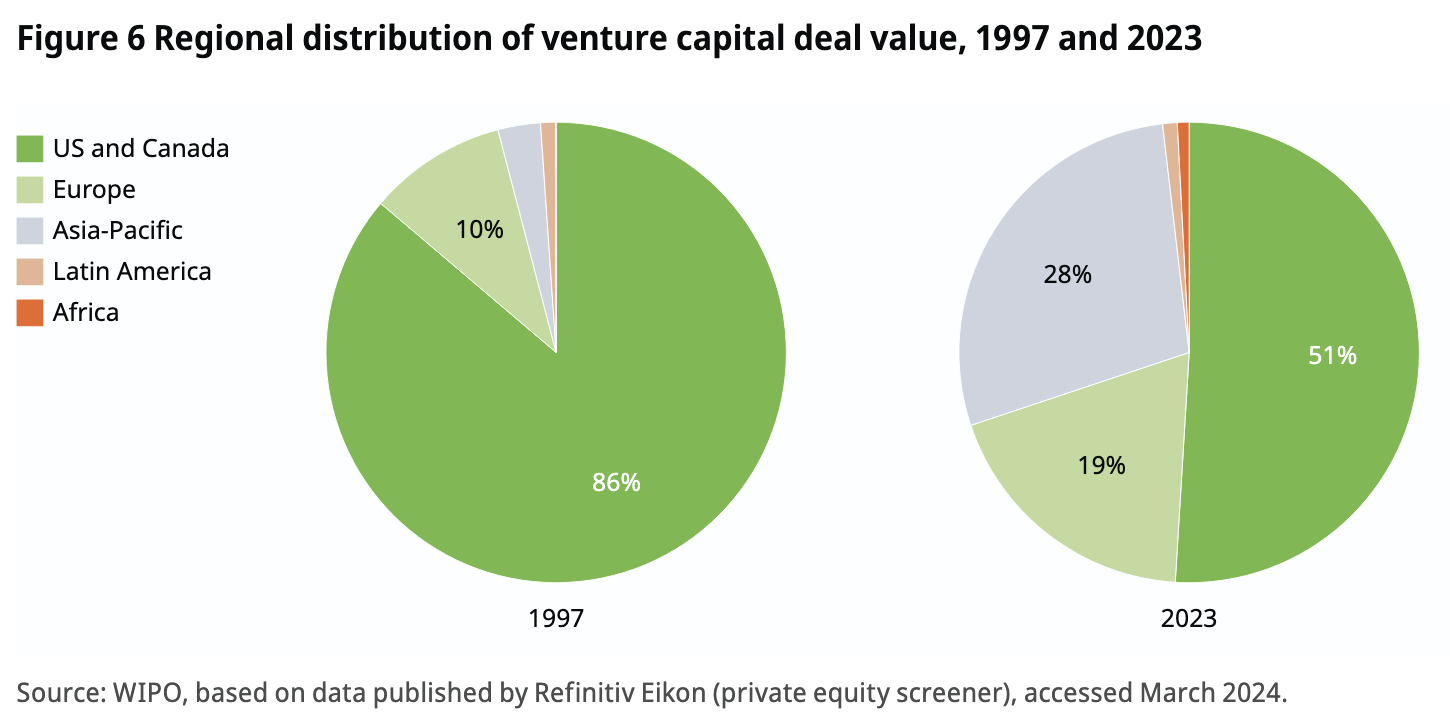
\includegraphics[width=\textwidth]{./assets/vc-gdp-share.png}
  \caption{Доля венчурного капитала в структуре ВВП развитых стран}
  \label{fig:vc-gdp-share}
\end{figure}

Анализ предметной области демонстрирует, что на этом этапе стоимость проектов формируется не реальными денежными потоками, а ожиданиями и верой участников экосистемы. Отсутствие стабильных финансовых показателей заставляет инвесторов полагаться на фрагментарные данные — результаты первых прототипов, отзывы пользователей, а порой и просто репутацию команды — что приводит к существенной информационной асимметрии.

% ### 1.2
\mysection{Определение актуальности}

Основатели стартапов сталкиваются с необходимостью быстрой проверки своих идей на жизнеспособность. Традиционные механизмы, такие как венчурный капитал или акселерационные программы, часто требуют длительных циклов отбора, раскрытия критически важной информации и подчинения строгим условиям, что создает барьеры для быстрой рыночной валидации. В то же время инвесторы, ориентированные на диверсификацию портфеля за счет перспективных, но еще не оформившихся инициатив, нуждаются в надежных инструментах для оценки широкого спектра проектов и оптимального распределения капитала. Текущие подходы, основанные на дискретных инвестиционных раундах, ограничивают выборку доступных стартапов и усиливают монополию крупных игроков, оставляя множество потенциально прорывных идей без поддержки.

Одной из ключевых проблем является информационная асимметрия между основателями стартапов и потенциальными инвесторами. Основатели обладают глубоким пониманием своих проектов, однако при необходимости привлечения инвестиций вынуждены подстраивать это понимание под маркетинговый контекст. В свою очередь, инвесторы ограничены в доступе к полной информации о проекте и его перспективах, что затрудняет объективную оценку и вынуждает опираться на косвенные сигналы, такие как образование и опыт основателей.

Особенно ярко это проявляется в блокчейн стартапах, ведь им необходим пул ликвидности для обеспечения бесперебойной торговли, стабильности цен и доверия пользователей к их токену или платформе. Пул ликвидности — это резерв цифровых активов, хранящийся в блокчейне и предназначенный для автоматического обмена токенов по заранее установленным правилам без участия посредников.

Обеспечение достаточного уровня ликвидности является фундаментальным условием эффективного функционирования блокчейн-стартапов, поскольку именно она обеспечивает непрерывность торговых операций, минимизирует проскальзывание и способствует поддержанию стабильности ценового уровня токена. Глубокая ликвидность выступает индикатором здоровой экосистемы, привлекает трейдеров, предпочитающих площадки с низкой ценовой волатильностью, и формирует доверие инвесторов к проекту, что, в свою очередь, усиливает сетевой эффект и стимулирует дальнейшее расширение пользовательской базы. При недостаточном объёме ликвидности даже незначительные сделки способны вызвать существенные колебания цены, создавая угрозу массового оттока участников и повышая риски ценовых манипуляций со стороны крупных держателей.

Достижение и поддержание необходимого уровня ликвидности осуществляется с помощью ряда финансовых и организационных подходов. В первую очередь, для быстрого привлечения средств используются программы, которые поощряют участников сообщества размещать свои активы в пулах за вознаграждение. Другим распространённым способом является первичное размещение токенов на децентрализованных биржах, позволяющее одновременно привлечь инвестиции и сформировать начальный резерв активов для торговли.

Также применяется подход, при котором сам проект выпускает специальные облигации или аналогичные финансовые инструменты, чтобы напрямую владеть ликвидностью, избегая зависимости от временных внешних вложений.

Ещё одним вариантом является привлечение профессиональных организаций, специализирующихся на создании ликвидности, что позволяет обеспечить необходимый объём активов для торговли без значительных собственных расходов проекта.

Дополнительно используется размещение токенов на крупных централизованных биржах при поддержке профессиональных участников рынка, что расширяет круг потенциальных инвесторов и повышает популярность проекта.

Наконец, важным методом выступает применение автоматизированных алгоритмов, которые обеспечивают непрерывное формирование цен и постоянный доступ участников к торговле, снижая при этом резкие колебания цены и увеличивая доверие пользователей к платформе.

Комплекс этих проблем создаёт существенные барьеры для эффективного функционирования рынка инвестиций в ранние стадии, приводя к неоптимальному распределению капитала, когда перспективные проекты остаются без необходимой поддержки, а проекты с меньшим потенциалом, но лучшей презентацией или более сильными социальными связями, получают непропорционально большие инвестиции, что в конечном итоге снижает эффективность инновационной экосистемы и замедляет технологический прогресс.

% ### 1.3
\mysection{Описание целевой аудитории}

Портрет целевой аудитории платформы включает в себя две ключевые группы: основателей стартапов и инвесторы, ориентированных на высокорисковые, но потенциально доходные вложения.

Первую группу составляют преимущественно молодые люди от 20 до 35 лет. Они нуждаются в доступе к капиталу, который должен основываться на объективной оценке потенциала идеи, а не на субъективных факторах, таких как опыт, образование или социальные связи, что подтверждается тем, Отсутствие качественной обратной связи представляет существенное препятствие для развития их проектов. Они стремятся минимизировать затраты времени и ресурсов на привлечение инвестиций, что особенно актуально, учитывая, что процесс привлечения посевного финансирования в среднем занимает от шести до девяти месяцев.

Вторую группу составляют инвесторы ранних стадий, для которых важным является обеспечение доступа к качественному потоку сделок с высоким потенциалом. Помимо этого, инвесторам необходимы объективные данные для оценки потенциала проектов в условиях ограниченного объёма информации; Наконец, инвесторы стремятся к диверсификации инвестиционного портфеля, предпочитая инвестировать в большое кол-во проектов, что позволяет распределить риски, несмотря на ограничения, связанные с оценкой большого количества проектов.

Учитывая, что обе группы действуют в условиях высокой неопределённости и переизбытка информации, внимание становится дефицитным ресурсом. Рынок инноваций и венчурного капитала всё чаще функционирует по законам экономики внимания, где первичную роль играет не только содержание, но и форма подачи. Визуально привлекательный, яркий, интуитивно понятный интерфейс становится не просто инструментом взаимодействия с продуктом, а критическим фактором захвата и удержания пользователя, особенно в условиях растущей конкуренции за внимание. Он способствует не только улучшению пользовательского опыта, но и формирует доверие к технологической и инновационной зрелости платформы.

Проведённый анализ целевой аудитории демонстрирует, что, несмотря на различия в потребностях, стейкхолдеры заинтересованы в создании более эффективной, объективной и прозрачной системы оценки и финансирования инновационных проектов на ранних стадиях. В этом контексте яркий, современный и эмоционально вовлекающий интерфейс представляет собой не эстетическую деталь, а стратегически важный инструмент, способствующий расширению аудитории, повышению вовлечённости пользователей и достижению маркетинговых целей на конкурентном рынке.

% ### 1.4
\mysection{Обзор существующих решений}

В современной экосистеме инвестирования применяются различные подходы, каждый из которых частично решает обозначенные проблемы, но не способен обеспечить

Основные практики привлечения инвестиций включают традиционное венчурное финансирование, участие в акселерационных программах, краудфандинг.

Венчурные фонды и инвесторы представляют собой наиболее распространённый механизм финансирования ранних стадий, основанный на личных встречах, презентациях и субъективной оценке потенциала проектов и команд. Преимущества данного подхода заключаются в наличии доступа к экспертной поддержке и менторству, возможности установления долгосрочных отношений между основателями и инвесторами, гибкости в структурировании сделок и условия инвестирования, а также наличии широкой сети контактов, которую инвесторы могут предоставить. Однако существенные ограничения этого механизма проявляются в высокой степени субъективности и предвзятости при оценке проектов, Согласно \cite{imbierowicz2024peer}, оценки стартапов на ранних стадиях часто опираются не на бизнес-фундамент, а на ориентиры из недавних сделок в смежных сегментах, что приводит к эффекту переоценки и рыночной нестабильности. Дополнительно, зависимость от социальных связей и репутации, а также необходимость полного раскрытия идеи, создающая риск для интеллектуальной собственности и географическая концентрация венчурных инвестиций, ограничивающая доступ к капиталу для основателей из других регионов, существенно снижают эффективность данного подхода.

Акселераторы и стартап-инкубаторы, такие как Y Combinator, Techstars, AngelList, предлагают структурированные программы поддержки стартапов, объединяющие менторство, образовательные компоненты и доступ к инвесторам. Структурированный процесс отбора и поддержки проектов создаёт чёткие рамки для развития, что особенно важно для неопытных основателей \cite{thiel2014zero}, а доступ к обширным сетям контактов и экспертизе ускоряет валидацию идей и выход на рынок. При этом частичная автоматизация инвестиционных процессов снижает транзакционные издержки, а стандартизация документации упрощает юридические аспекты финансирования. Главной проблемой здесь является высокая конкуренция за места в ведущих программах (например, Y Combinator принимает менее 1\% заявителей \cite{yc_acceptance_rate}) значительно снижает шансы на участие и отсеивает потенциально хорошие идеи. Также, географические ограничения продолжают оставаться барьером для основателей, расположенных вне основных инновационных хабов.

Альтернативными механизмами являются платформы краудфандинга, которые способствуют демократизации доступа к инвестициям, позволяя привлекать финансирование без зависимости от традиционных связей, а также обеспечивают валидацию идеи через прямой отклик потенциальных пользователей. Такие подходы также способствуют созданию сообщества вокруг проекта на ранних стадиях, однако часто решения о финансировании принимаются исключительно за счет маркетингово продвижения, что может приводить к поддержке коммерчески нежизнеспособных проектов. По данным отчёта KingsCrowd \cite{kc2024}, несмотря на постепенное снижение общего объёма инвестиций в рамках краудфандинга (рисунок ~\ref{fig:crowd-funding}), количество инвестиционных сделок демонстрирует устойчивый рост (рисунок ~\ref{fig:crowd-funding}). Это указывает на рост популярности малых инвестиционных раундов.

\begin{figure}[H]
  \centering
  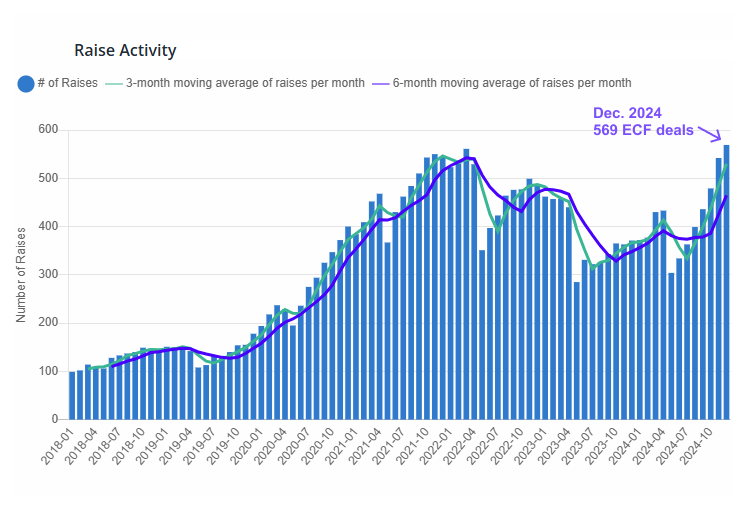
\includegraphics[width=0.9\textwidth]{./assets/crowd-funding.png}
  \caption{Рост числа инвестиций}
  \label{fig:crowd-funding}
\end{figure}

Сравнительный анализ эффективности существующих подходов показывает, что ни один не способен обеспечить одновременно, объективную оценку проектов и оптимальное распределение капитала. Стоит отметить, что сильной стороной традиционных подходов является их структурированность и наличие экспертной поддержки, особенно в случае венчурных фондов и акселераторов, где стартапы получают доступ к опыту и связям \cite{lange2024angels}. Однако слабые стороны этих механизмов существенно ограничивают возможности их масштабирования.

% ### 1.5
\mysection{Требования к технической реализации}

Функциональные требования:
\begin{enumerate}
  \item Система должна предоставлять пользователю способ отправлять идею и делать её доступной для коллективной оценки.
  \item Пользователи должны иметь возможность выражать интерес к идее, влияя на её развитие и видимость.
  \item Идеи должны получать рыночную оценку.
  \item Администратор должен иметь возможность валидировать контент до его публикации на платформе.
  \item Система должна адаптироваться к изменению поведения участников для поддержания честности и эффективности.
\end{enumerate}

Нефункциональные требования:
\begin{enumerate}
  \item Совместимость: поддержка iOS, Android, Web и Telegram Mini Apps.
  \item Производительность: время отклика системы не должно превышать 30 секунд.
  \item Прозрачность: все финансовые операции и решения фиксируются в смарт-контрактах на публичном блокчейне.
  \item Модульность: архитектура должна быть компонентной с возможностью обновления, замены и масштабирования отдельных частей.
\end{enumerate}

% ### 1.6
\mysection{Вывод по первой главе}

Таким образом, проведенный анализ указывает на необходимость создания комплексного механизма, который бы одновременно обеспечивал объективную оценку проектов и оптимальное распределение капитала с учётом как объёма инвестиций, так и широты поддержки аудиторией.

% Глава 2
% ###############################################################
\mychapter{ТЕОРЕТИЧЕСКИЕ ОСНОВЫ РАСПРЕДЕЛЕНИЯ РЕСУРСОВ}

Глава посвящена теоретическим моделям и принципам построения механизмов распределения ресурсов, анализу составных частей, необходимых для создания подобных систем.

% ### 2.1 Обзор проблематики
\mysection{Обзор проблематики}

Проблема распределения ресурсов охватывает широкий спектр дисциплин — от найма персонала и управления проектами до вычислительных систем, логистики и сетевой инфраструктуры. В формальном виде она сводится к оптимизации под ограничениями, где множество допустимых решений экспоненциально возрастает с ростом количества агентов, ресурсов и ограничений. При этом большинство задач относятся к классу NP-трудных, что делает невозможным их точное решение в разумное время и требует приближённых или эвристических подходов.

Даже в системах с чётко определёнными и конечными правилами возникает экспоненциальный рост числа допустимых состояний. Например, в настольной игре «го» количество возможных позиций оценивается в порядке $10^{170}$, что значительно превышает любые физические пределы обработки. Аналогично, алгоритм AlphaZero \cite{silver2018general}, хотя и оперирует в рамках формализованных правил, демонстрирует, что оптимальное поведение в таких пространствах возможно лишь при использовании стохастических методов и обучения с подкреплением, поскольку алгоритмический перебор стратегий неосуществим.

Таким образом, несмотря на конечность правил и чёткую формализацию условий, многие реальные системы распределения ресурсов становятся неалгоритмизируемыми в силу экспоненциальной сложности и стратегической природы агентов. Это обосновывает необходимость перехода к децентрализованным, эмпирическим и конкурентным механизмам, которые перераспределяют вычислительную нагрузку, используют локальную информацию и допускают адаптивное поведение участников.

% ## 2.2
\mysection{Экономические принципы}

Рыночные механизмы — одна из самых ранних систем распределения, возникших естественным образом из человеческой потребности в обмене ресурсами. Рынки представляют собой уникальный пример высокоэффективной распределённой системы, сформированной не посредством централизованного планирования, а в результате спонтанной самоорганизации. Исторически развитие рынков сопровождалось появлением новых форм коммуникации — от устных соглашений и письменных контрактов до телеграфа и цифровых платформ. Эти инновации способствовали расширению информационной пропускной способности рынков и увеличению точности передаваемых сигналов. В процессе обмена участники взаимодействуют в общих физических или цифровых пространствах — от рыночных площадей до онлайн-бирж — в результате чего формируется ключевой институциональный механизм: рыночная цена. Изначально сделки совершаются по индивидуально согласованным условиям, но с ростом числа участников рынок агрегирует информацию, и цены стремятся к единственному значению, отражающему консенсус оценок (рис.~\ref{fig:one-price}). Такая цена становится выражением коллективного знания, интегрируя разрозненные субъективные взгляды в объективный показатель. В самом простом примере когда два человека обмениваются товарами, они должны согласиться о его цене. Получается цена передает наши знания о ценности товара которые мы продаем и веру в ценность товара которые мы получаем. Как только большее число игроков присоединяется к обмену, то цена становится консенсусом и другим уже не нужно спорить о цене, она уже установлена в каких-то приделах и ценой можно воспользоваться как сервисом.

\begin{figure}[H]
  \centering
  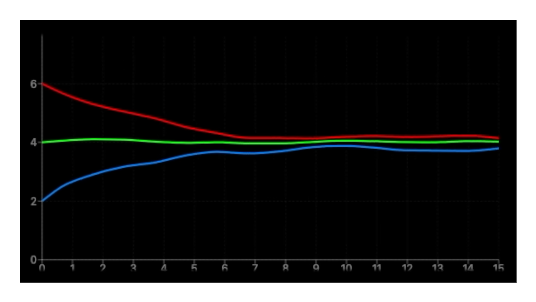
\includegraphics[width=0.9\textwidth]{./assets/one-price.png}
  \caption{Сходимость ценовых ожиданий участников рынка}
  \label{fig:one-price}
\end{figure}

Ключевой особенностью рынка является то, что он не требует от участников доверять друг другу. Цена саморегулируется. Вопреки ожиданиям, доступ к конфиденциальной информации не искажает рыночный сигнал. Наоборот, с точки зрения экономической теории, такие действия способствуют увеличению точности ценовых индикаторов. Участник, обладающий частной информацией, скрытыми знаниями или уникальной экспертизой стремится извлечь из неё выгоду, тем самым внося её в общедоступную цену, что в конечном итоге усиливает достоверность рыночных прогнозов.

Это свойство можно легко заметить, если сравнить графики глубины рынка для торговых пар с высокой и низкой ликвидностью (рис.~\ref{fig:limit-order}). Выраженная симметрия и плотность книги заявок в низколиквидных торговых парах свидетельствуют о высокой степени уверенности и согласованности ожиданий рыночных участников.

\begin{figure}[H]
  \centering
  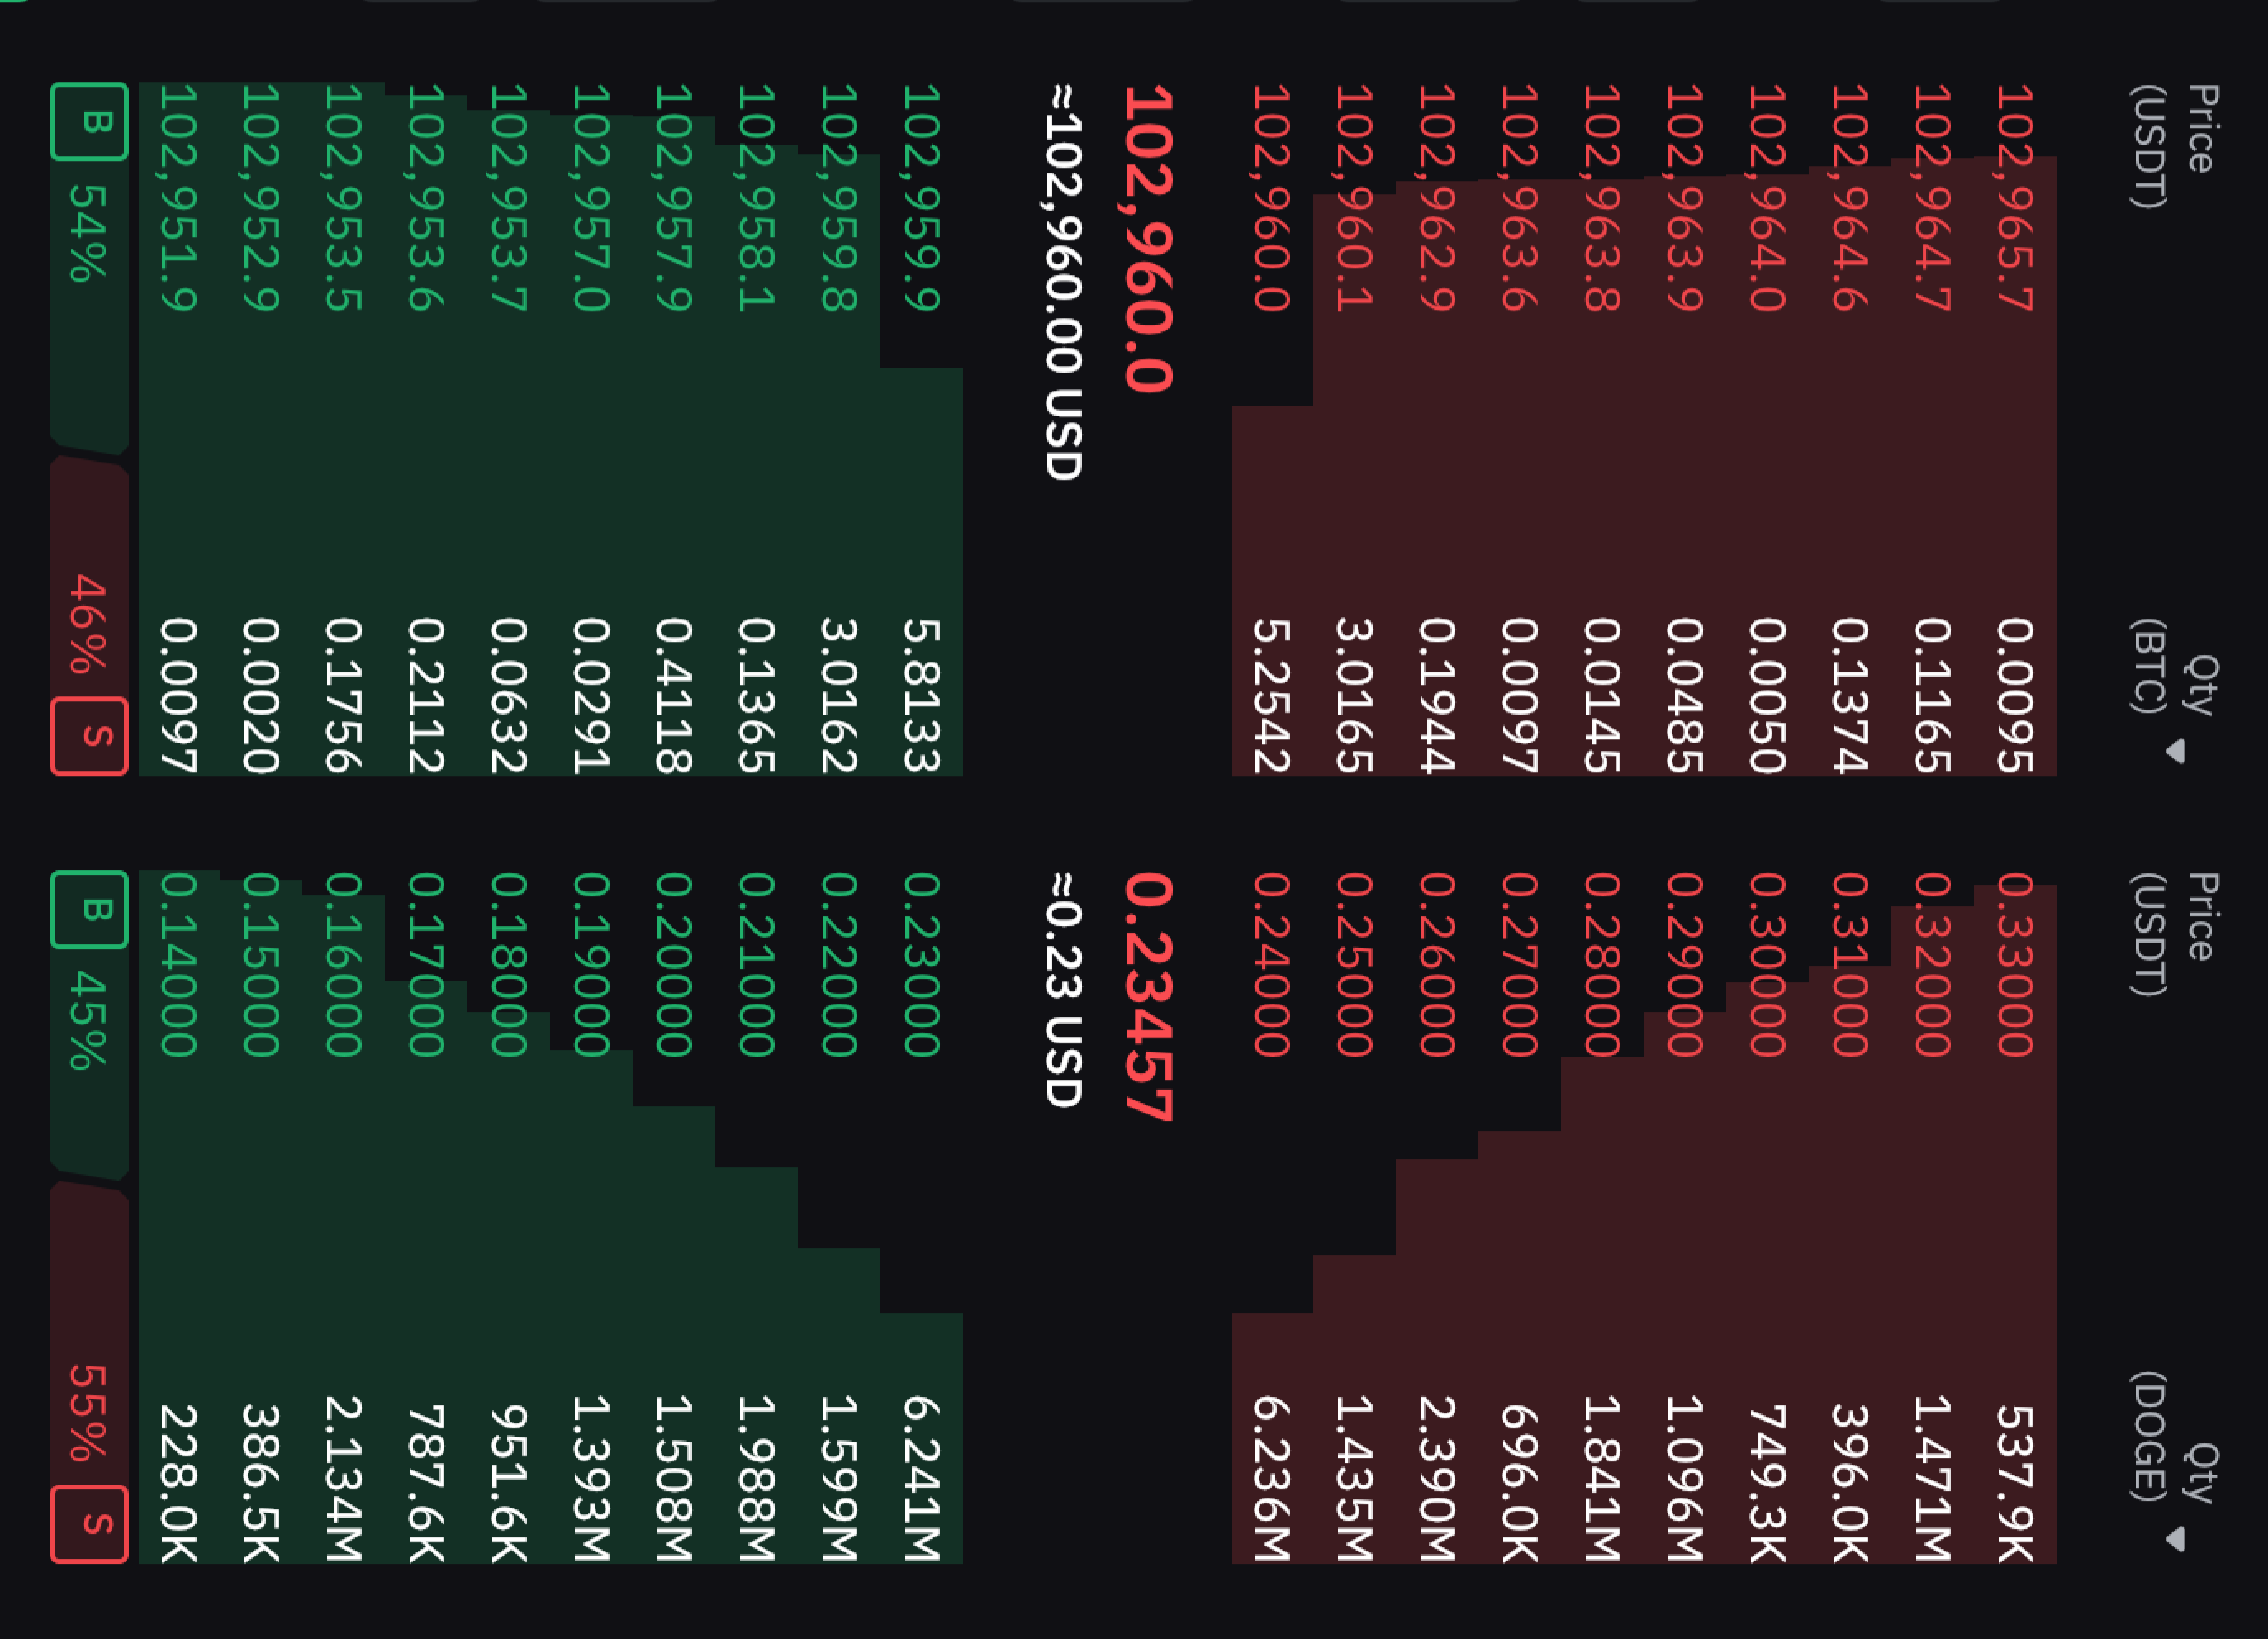
\includegraphics[width=0.9\textwidth]{./assets/limit-order.png}
  \caption{График глубины рынка для торговых пар с высокой и низкой ликвидностью}
  \label{fig:limit-order}
\end{figure}

Это происходит из-за того что рынок это равновесная среда.

В этом контексте возникает важный вопрос: что произойдет, если мы отбросим настоящий компонент ценообразования и будем основывать торги только на будущих событиях. Отражение будущих ожиданий в ценах особенно ярко проявляется в таких примерах, как изменение стоимости фьючерсов на сельскохозяйственную продукцию в ответ на погодные прогнозы или изменение коэффициентов в букмекерских системах до фактического события \cite{wolfers2019price}. Тогда мы избавляемся от текущей компоненты стоимости и цена начинает полностью отражать вероятность. Таким образом, рыночные цены становятся не просто индикатором текущего состояния, но и носителем предсказательной информации о будущем.

Одним из современных применений предсказательных рынков является проект Polymarket, использующий блокчейн для создания прозрачных и децентрализованных платформ прогнозирования.Самый известный прогноз Polymarket на сегодняшний день - президентские выборы в США в 2024 году за несколько недель до того, как стал известен результат. В результате системы такого рода обеспечивают высокий уровень точности предсказаний.

\begin{figure}[H]
  \centering
  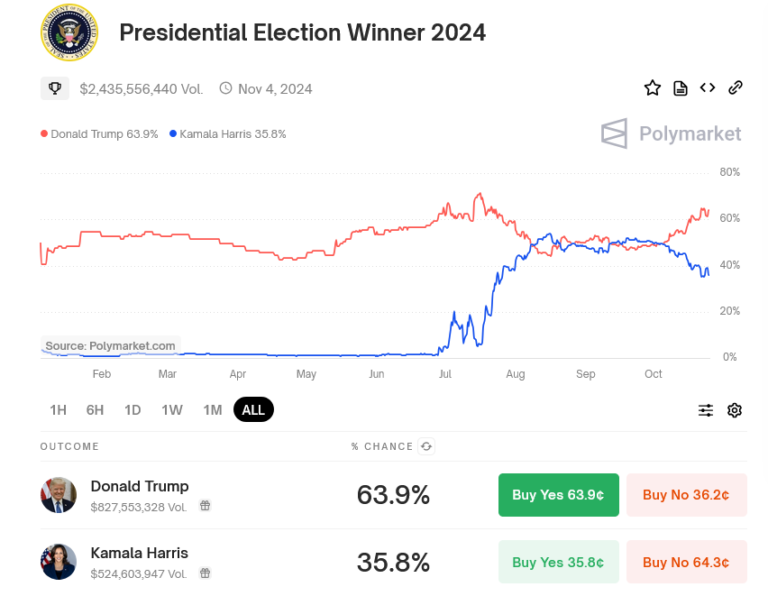
\includegraphics[width=0.9\textwidth]{./assets/polymarket-elections.png}
  \caption{Прогноз президентских выборов в США в 2024 году}
  \label{fig:polymarket-elections}
\end{figure}

Данные результаты демонстрируют возможность использования рыночных механизмов для предсказания будущих событий, а объединение традиционных рыночных механизмов с системами аналитики и вычислительными платформами формирует новую парадигму коллективного интеллекта \cite{berg2020prediction}.

Попробуем разобрать составные части подобных систем, чтобы получить представление о системе распределения ресурсов \ref{fig:bpmn-new}.

\begin{figure}[H]
  \centering
  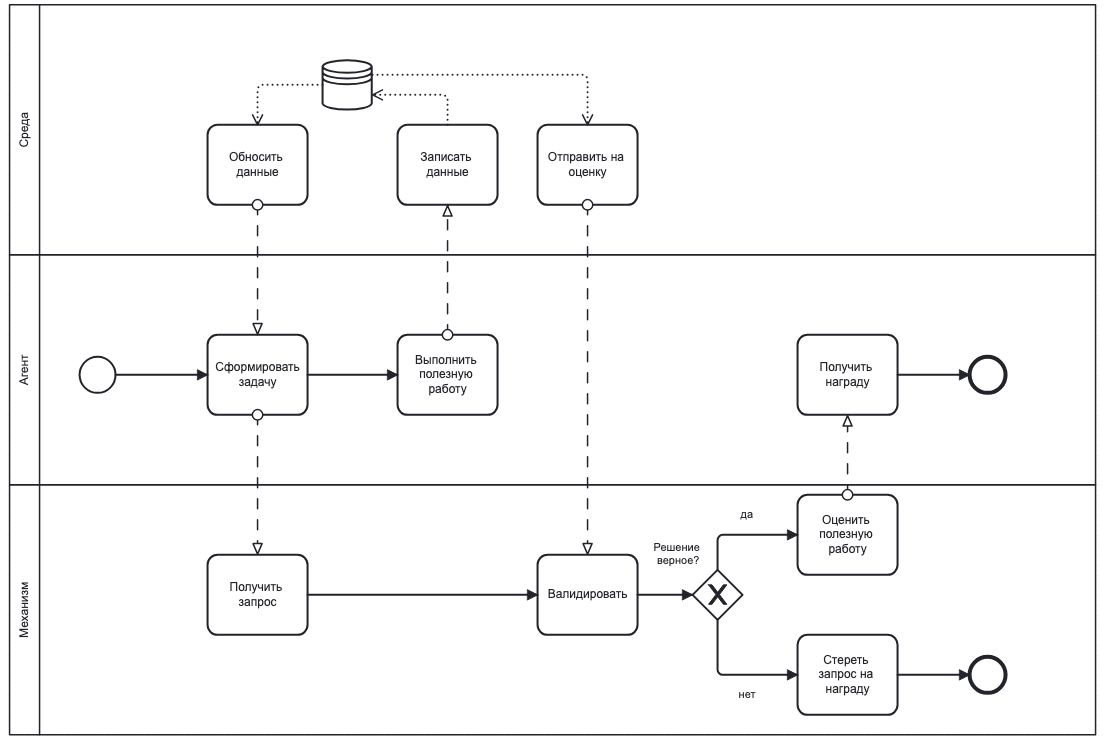
\includegraphics[width=0.8\textwidth]{./assets/bpmn-new.png}
  \caption{Формальная схема процесса распределения ресурсов}
  \label{fig:bpmn-new}
\end{figure}

% ## 2.3
\mysection{Вычислительная мощность}

% Цена отражает знания о товаре и ожидание о полученном

Другими необходимым условием для того, чтобы механизм работал является наличие у агентов локальных экспертиз и отсутствие баесов при принятии решений;

Каждый агент выполняет полезную работу, формируя выходные данные.
Через механизм согласования эти действия агрегируются в глобальное состояние, по которому затем все агенты синхронизируют новую итерацию.

Необходимо заинтересовать агентов в выполнении полезной работы, так как любые косвенные или иерархические системы уступают прямому большинству (дестилляции коллективного знания) — прямой мажоритарной системе — по вероятности принятия «правильного» решения при условии независимости голосов и компетентности участников (p>0.5). Это демонстрирует, что децентрализованный рынок (прямое большинство) доминирует над всеми промежуточными схемами.

Согласно «Сondorcet's jury theorem» \cite{condorcet1785essay}, если у каждого участника системы вероятность дать правильную оценку чуть выше 50\%, то объединённое мнение группы с экспоненциальной вероятностью стремится к истине по мере роста размера группы.

Если даже индивидуальный агент обладает ограниченной информацией и баесом, при условии что участники системы заинтересованны давать правильные предсказания, при отсутствии координированных искажений, агрегирует разнообразные частичные знания, формируя более точное представление о будущем событии.

\begin{figure}[H]
  \centering
  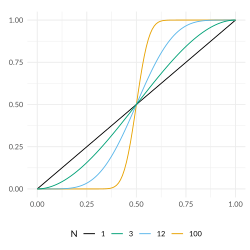
\includegraphics[width=0.5\textwidth]{./assets/condorcent.png}
  \caption{Вероятность для нескольких групп P преуспеть}
  \label{fig:condorcet}
\end{figure}

Следовательно, для эффективного функционирования механизма требуется трансформировать вероятностную модель, формируя такую экономическую среду, в которой соблюдение установленных правил становится единственной рациональной стратегией для участников.
Ключевым требованием является стимулирование агентов к выдаче максимально точных результатов. Если каждый агент обладает вероятностью $p > 0.5$ дать корректную оценку, то вероятность того, что большинство из $n$ участников примет правильное решение, вычисляется по формуле
\[
  \text{Pr}(\text{большинство правильно}) = \sum_{k=\lceil n/2 \rceil}^{n} \binom{n}{k} p^k (1-p)^{n-k},
\]

и при $p > 0.5$ стремится к единице по мере роста $n$. В иерархических или рекурсивных системах, где выход одних агентов служит входом для других, общая вероятность корректного результата по цепочке длины $k$ равна произведению
\[
  p_1 \times p_2 \times \cdots \times p_k,
\]

и остаётся выше $0.5$ для небольших $k$, если все $p_i > 0.5$. Более того, при наличии нескольких независимых путей вычисления итогового результата совокупная вероятность правильности определяется суммой соответствующих произведений, что дополнительно усиливает надёжность механизма.


%% ## 2.4
\mysection{Рациональная стратегия}

Равновесие Нэша является важным понятием в теории игр, так как оно определяет стабильные результаты в играх с несколькими участниками, где каждый игрок принимает решения, основываясь на ожиданиях других игроков. Это помогает анализировать и предсказывать поведение игроков в различных ситуациях, таких как конкуренция, сотрудничество и кооперация.

% TODO: общее экономическое равновесие supply/demand
\begin{figure}[H]
  \centering
  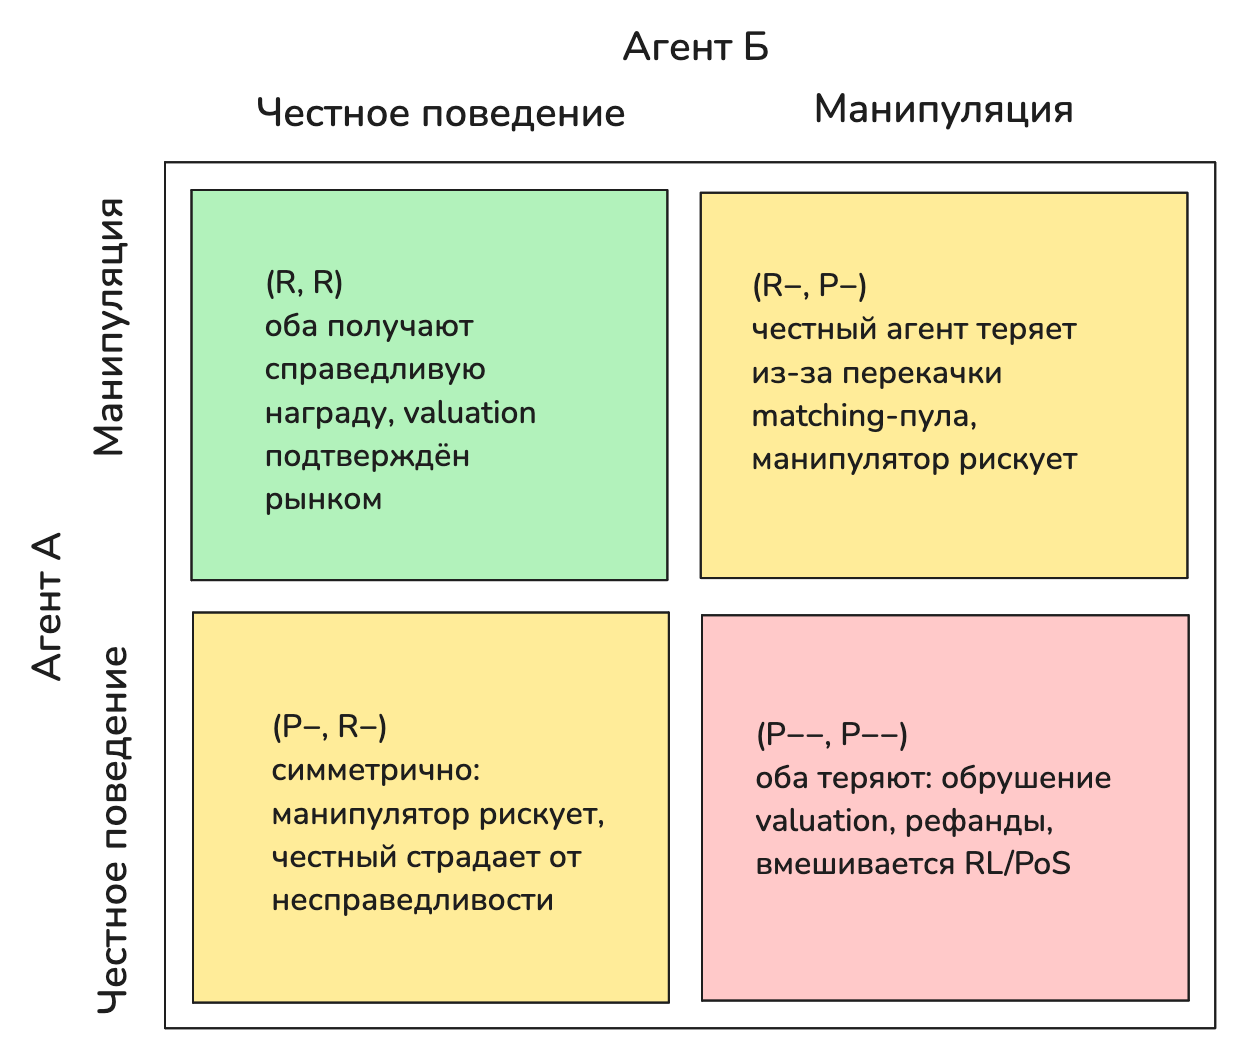
\includegraphics[width=0.5\textwidth]{./assets/nash-equilibrium.png}
  \caption{Равновесие Нэша}
  \label{fig:nash-equilibrium}
\end{figure}

В поученной системе распределения ресурсов ни один агент не может изменить свое решение так, чтобы увеличить свою выгоду, не ухудшая при этом результаты других игроков. Другими словами, в равновесии Нэша каждый агент выбирает стратегию, которая максимизирует его собственную выгоду, учитывая стратегии, выбранные другими агентами.

% ## 2.5
\mysection{Система управления}

Примером является государственное регулирование экономической активности.
В экономике таким механизмом является центральный банк, который контролирует инфляцию и дефляцию.

Ярким историческим примером нетрадиционной денежной политики служит эксперимент с «свободными деньгами», проведённый в австрийском городе Вергль в 1932-1933 гг. В условиях дефляционного кризиса Великой депрессии местные власти ввели местную валюту с отрицательной процентной ставкой. Каждая банкнота теряла 1\% своей стоимости ежемесячно, что стимулировало быстрый оборот денег. По данным муниципальной статистики, за 13 месяцев эксперимента объём торгов вырос на 220\%, безработица сократилась на 25\%, при этом инфляция оставалась контролируемой \cite{stodder1998worgl}. Этот опыт демонстрирует потенциал альтернативных денежных систем в условиях кризиса ликвидности.

Тк мы не можем построить модель которая апроксимирует весь рынок целиком, нам необходимо адаптировать модель под изменяющиеся условия

Рассмотрим на примере самых простых механизмов которые теоретически можно использовать для решения подобных проблем.

На первым будет централизованная система, в которой все решения принимает единый ИИ-агент. Такой подход обеспечивает простоту архитектуры и быструю реакцию на входные данные, а также возможность эффективно обрабатывать конфиденциальную информацию без её публичного раскрытия. Однако он нарушает принципы достоверной нейтральности: весовые коэффициенты модели содержат скрытые предпочтения, сама модель остаётся непрозрачной ввиду колоссальной сложности, а частые обновления (примерно каждые три месяца) создают дополнительную нагрузку на сопровождение и могут вносить непредсказуемые сдвиги в принятие решений.

Противоположный предел это Футархия \cite{Hanson2000}, которая опирается на рынки прогнозов, предполагая, что свободная торговля информацией порождает наилучшие коллективные решенияю однако именно эта зависимость от торговли делает механизм уязвимым. Во-первых, ликвидность предсказательных контрактов редко бывает достаточной: если объём ставок невелик, даже умеренный игрок может заметно сместить цену, получить ложный сигнал и повлиять на итог, не понеся сопоставимых издержек \cite{Othman2013}. Во-вторых, котировка отражает ожидания только тех, кто готов поставить средства публично; участники с крупной приватной информацией могут предпочесть не раскрывать её, опасаясь законодательных рисков или репутационных потерь, и тогда рынок теряет часть знания, которое должен был агрегировать \cite{Pennock2011}. Третья важная проблема связана с выбором метрики: если показателем «успеха» политики служит одно число, агенты начинают оптимизировать именно его, даже в ущерб менее измеримым, но социально значимым факторам, а рынок прогнозов по-прежнему оценивает лишь формально заявленный показатель. Кроме того, футархия предполагает, что окончательное наступление проверяемого события отделено во времени от решения о политике; в этот период могут измениться внешние условия, подрывая связь между ставкой и реальным благом. Пока событие не решено, капитал участников заблокирован, и для долгих горизонтов это существенно повышает альтернативные издержки, чем ограничивает число желающих участвовать в прогнозе. Наконец, нормативная среда остаётся препятствием: законодательство многих стран приравнивает рынки предсказаний к азартным играм, что вводит ограничения на размер позиции, перечень событий и географию доступа, тем самым снова снижая участие и усложняя глобальное агрегирование информации \cite{Buterin2025}.

Если рассматривать все возможные задачи оптимизации или классификации (с одинаковой вероятностью), то любой алгоритм, который хорошо работает на одних задачах, неизбежно будет хуже на других. Иными словами, средняя производительность всех алгоритмов по всем возможным задачам одинакова \cite{wolpert1996lack}. Теорема «небесплатного обеда» (No Free Lunch) для поиска и оптимизации утверждает, что при неизвестном заранее распределении задач никакой алгоритм (включая гибридные или промежуточные механизмы) в среднем не превзойдёт оптимальную стратегию по всем возможным задачам: любой выигрыш на одном классе проблем компенсируется проигрышем на другом.
Для любого алгоритма $A$, среднего значения ошибки $E_A(f)$ по всем возможным функциям $f \in F$:
\begin{equation}
  \sum_{f \in F} E_A(f) = \sum_{f \in F} E_B(f),
\end{equation}
где $E_A(f)$ — ошибка алгоритма $A$ на функции $f$.

Следовательно, промежуточные формы и не смогут одновременно достичь преимуществ обоих пределов на всех задачах, и при отсутствии дополнительной информации нельзя сделать выбор в пользу тог ту или иную сторону.

\begin{figure}[H]
  \centering
  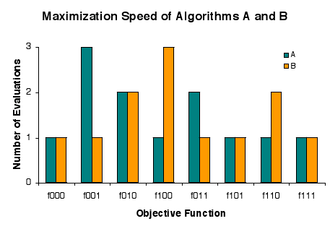
\includegraphics[width=0.5\textwidth]{./assets/freemeal.png}
  \caption{Иллюстрация теоремы о бесплатном обеде}
  \label{fig:free-meal}
\end{figure}

Таким образом, оптимальный механизм должен быть построен таким образом, чтобы учитывать возможность влияния на агентов возможность агентов выполянть определенные действия.

% ## 2.5
\mysection{Вывод по второй главе}

Класс система состоит из трех частей:
\begin{enumerate}
  \item Агент
  \item Среда
  \item Механизм
\end{enumerate}

Рассмотренная модель демонстрирует, что при корректной настройке стимулов и доверенного центра согласования можно получить механизм, способный адаптироваться к изменениям среды и масштабироваться за счёт множества заинтересованных агентов. Условием успеха является обеспечение вероятности правильных оценок каждого участника выше 50\%, что гарантирует надёжность принятия решений большинством и по цепочкам зависимостей.

% #####################################################
% Глава 3
\mychapter{ИНВЕСТИЦИОННОЙ ОЦЕНКА ЧЕРЕЗ МАСШТАБИРОВАНИЕ МОДЕЛИ}

Описанная в предыдущей главе модель может быть применена в рассматриваемой предметной области. В этой главе описывается формализация предметной области, математические модели и механизмы масштабирования распределения инвестиций с учётом поведения агентов.


Цена токена задаётся ABC на каждом этапе — это «постоянный» valuation, отражающий спрос и предложение в реальном времени.
Через burn-механизм ABC инвестор гарантированно может продать токены обратно в пул по алгоритмической цене.
Через PoS-стейк и вестинг создаётся долгосрочный интерес и препятствие для манипуляций.

Так как в системе создаются новые идеи без скрытых знаний это не будет влиять оценку агентов. Но в перспективе данную модель можно использовать при реальном рыночном анализе, где значения X и могут быть манипулированы. Почему я создаю изолированную систему: Новые идеи не подвержены скрытым знаниям (Y), что помогает не искажать модель.

Индивидуальный инвестор ограничен собственной неполной информацией и когнитивными искажениями. Однако группа агентов, действующая без скоординированных манипуляций, эффективно агрегирует частичную информацию, формируя более точное представление о перспективности стартапа. У участников системы есть скрытые знания о стартах, которые они мотивированы применить, чтобы забрать награду.
Даллее формализуем и рассмотрим каждую из частей по отдельности.

Таким образом, система реализует экономическое равновесие в ончейн-среде, где честное поведение становится доминирующей стратегией, а манипуляции ограничиваются структурными барьерами. Это позволяет масштабировать механизм распределения капитала, поддерживая устойчивость, прозрачность и справедливость принятия решений.

% ## 3.1
\mysection{Описание бизнес-процессов}

Чтобы понять каким образом построисть токеномику рассмотрим основные бизнес процессы.

\mysubsection{Адаптация механизма}
Консенсус наследуется от блокчейна. Инвесторы и авторы доверяют друг другу и не могут манипулировать механизмом.

В качестве агента мы буделм использовать пользователей.

Механизмом является нейросетевая модель обучения с подкреплением для балансировки интересов инвесторов и авторов

Верхнеуровневая структура система представлена на рисунке~\ref{fig:idef0}.

\begin{figure}[H]
  \centering
  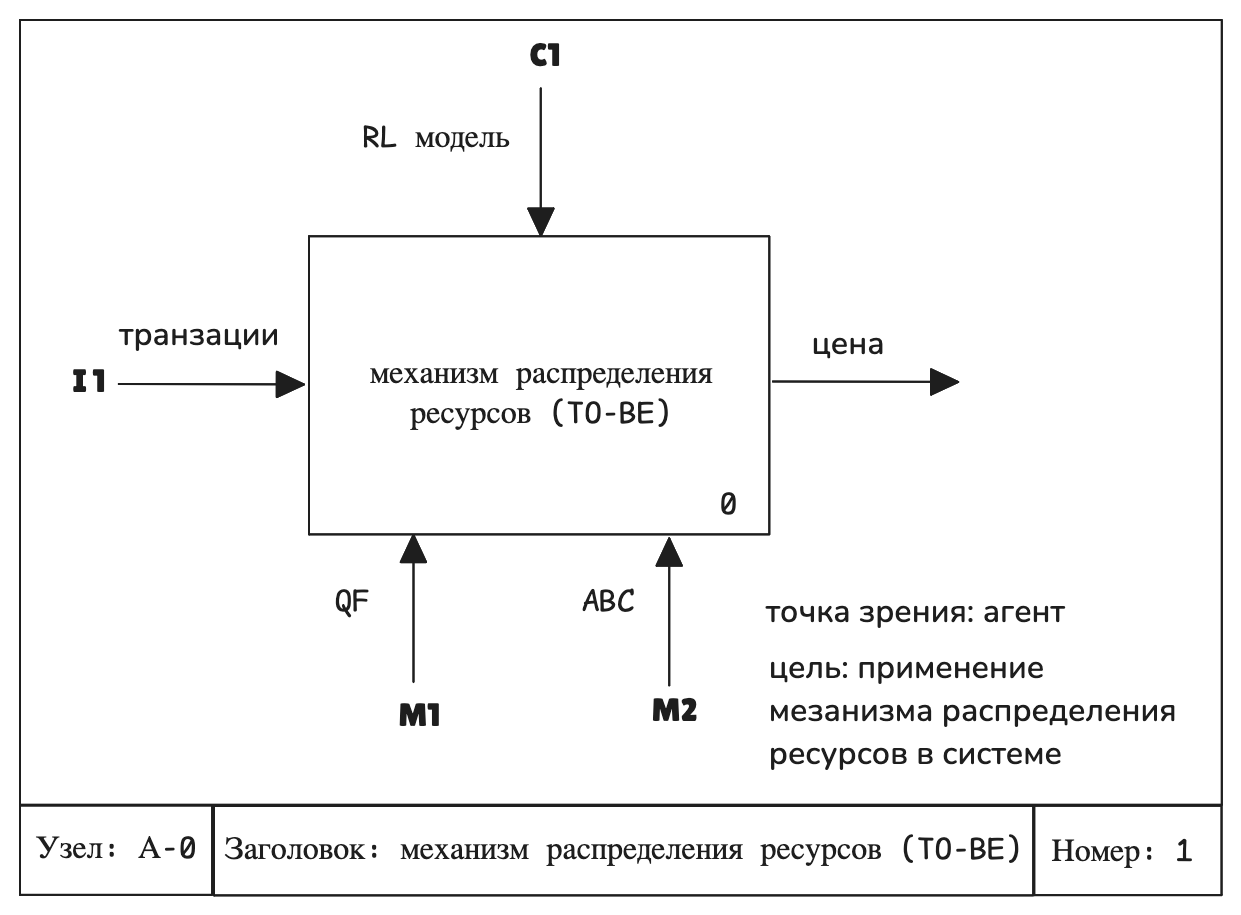
\includegraphics[width=0.9\textwidth]{./assets/idef0-A0.png}
  \caption{Механизм распределения ресурсов в нотации IDEF0 A0}
  \label{fig:idef0-A0}
\end{figure}

Рассмотрим составные элементы системы:
\begin{enumerate}
  \item Входы (Input) -- данные, частные знания или сигналы окружения необходимые для выполнения функции.
  \item Управление (Control) -- правила, политики или условия, управляющие функцией.
  \item Выходы (Output) -- результаты выполнения функции.
  \item Механизмы (Mechanism) -- стимулы для добровольного участия и согласования локальных решений в единую глобальную норму.
\end{enumerate}

После декомпозиции это выглядит так:

\begin{figure}[H]
  \centering
  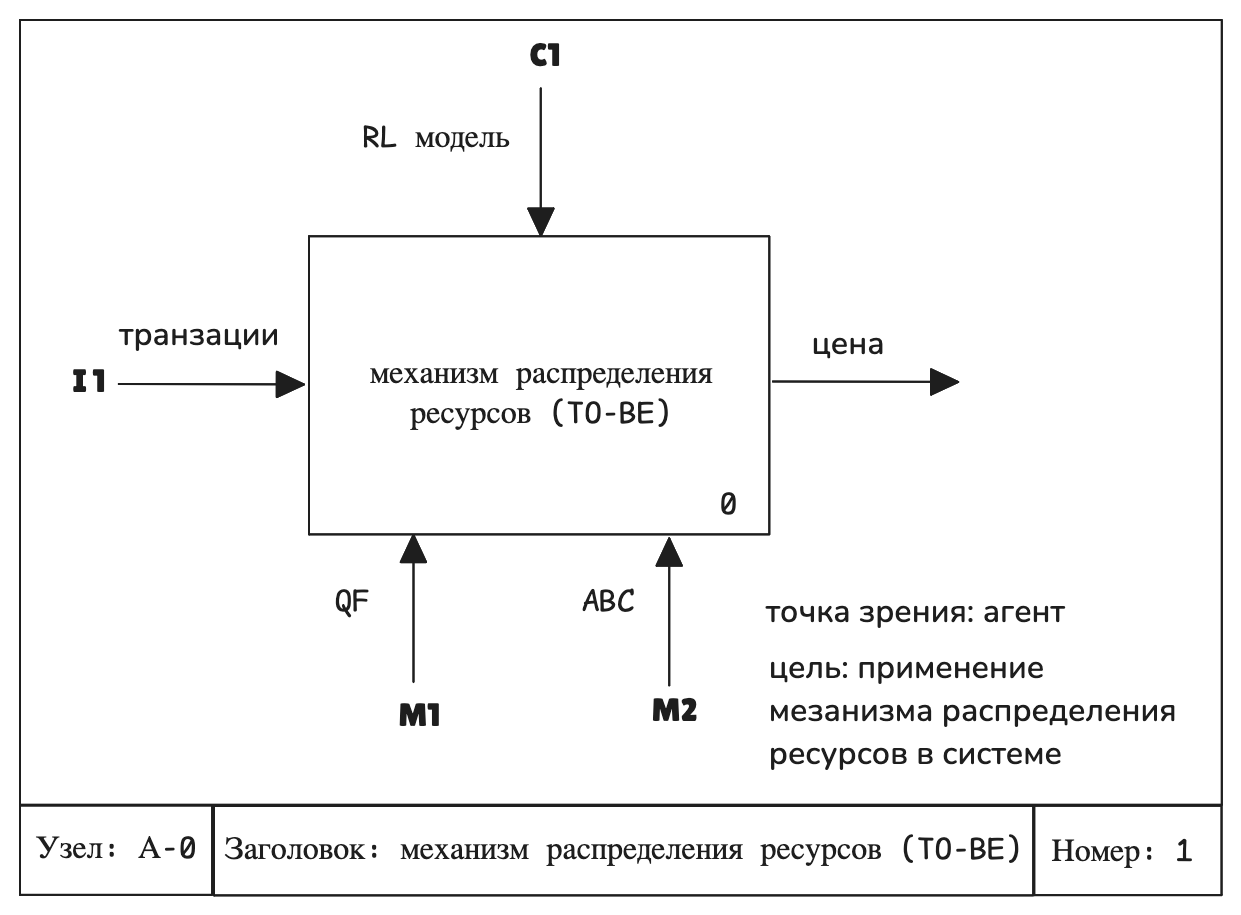
\includegraphics[width=0.9\textwidth]{./assets/idef0.png}
  \caption{Механизм распределения ресурсов в нотации IDEF0}
  \label{fig:idef0}
\end{figure}

\mysubsection{UML-модель механизма распределения ресурсов}

Для более наглядного представления модели распределения ресурсов в приложении была разработана UML-диаграмма вариантов использования (use case diagram), представленная на рисунке \ref{fig:uml-use-case-diagram}. Данная диаграмма демонстрирует взаимодействие различных акторов системы и распределение ролей между алгоритмическими и человеческими компонентами.

\begin{figure}[H]
  \centering
  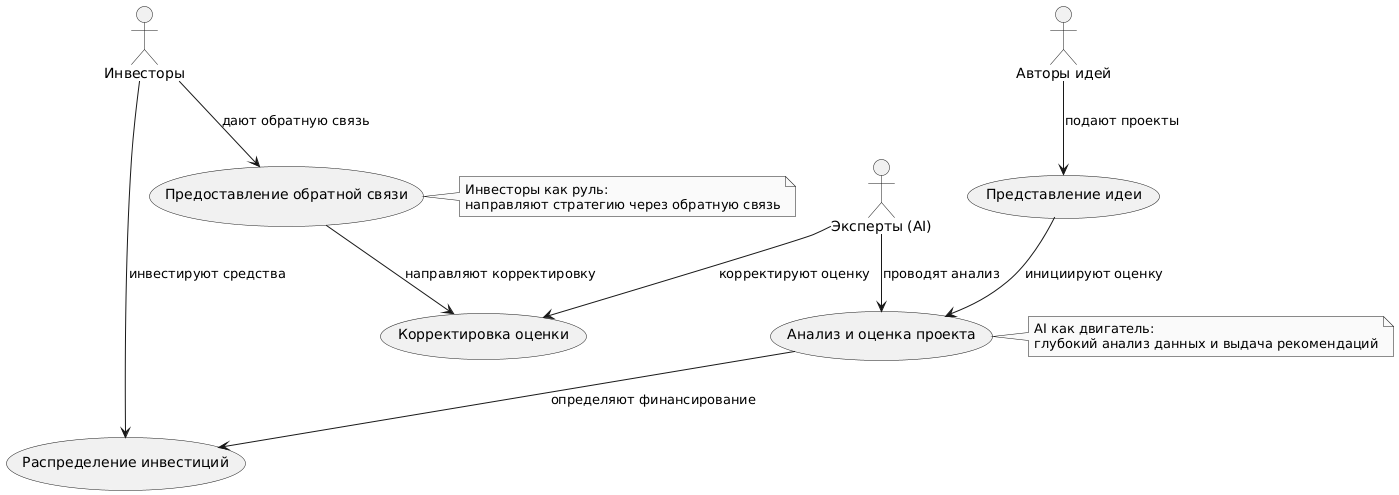
\includegraphics[width=0.9\textwidth]{./assets/uml-use-case-diagram.png}
  \caption{UML-диаграмма вариантов использования механизма распределения ресурсов с балансом автоматизации и человеческого контроля}
  \label{fig:uml-use-case-diagram}
\end{figure}

Как видно из диаграммы, в системе выделяются три основных группы участников: инвесторы, авторы идей и эксперты (представленные, в том числе, системами ИИ). Инвесторы участвуют в процессе предоставления обратной связи и непосредственного инвестирования средств, что направляет стратегию распределения ресурсов. Авторы идей подают свои проекты на рассмотрение через механизм представления идеи. Эксперты, включая аналитические системы на основе ИИ, выполняют ключевую роль по анализу и оценке проектов, а также корректировке предварительных оценок.

Центральными процессами в системе являются:

\begin{enumerate}
  \item Представление идеи -- процесс, при котором авторы формулируют и загружают свои проекты в систему.

  \item Анализ и оценка проекта -- основная аналитическая работа по многомерной оценке потенциала проекта, выполняемая в значительной степени автоматизированными системами с глубоким анализом данных.

  \item Предоставление обратной связи -- процесс, в котором инвесторы выражают свои предпочтения и видение направления развития.

  \item Корректировка оценки -- механизм коррекции и уточнения, где эксперты и инвесторы могут скорректировать предварительные результаты анализа.

  \item Распределение инвестиций -- финальный этап, на котором средства распределяются между проектами на основе комплексной оценки, полученной в результате работы механизма.
\end{enumerate}

Особенно важно отметить, что механизм построен по принципу, где алгоритмические компоненты выполняют основную вычислительную работу по обработке больших объемов данных, а человеческие компоненты направляют стратегию через обратную связь, определяют стратегические приоритеты и осуществляют контроль. Такой подход обеспечивает баланс эффективности и надежности, сочетая вычислительную мощь алгоритмов с ценностями и экспертизой человеческих участников.

Данный механизм реализует принцип коллективного принятия решений, где автоматизация используется для обеспечения объективности и масштабируемости, а человеческое участие – для стратегического управления процессом и сохранения этических аспектов распределения ресурсов.

\mysubsection{Процессная модель масштабированного механизма инвестирования}

В целях формализации и визуализации бизнес-процессов функционирования масштабированного механизма инвестирования была разработана BPMN-диаграмма (Business Process Model and Notation), представленная на рисунке \ref{fig:bpmn}. Данная диаграмма иллюстрирует композицию взаимодействий между ключевыми участниками системы и последовательность выполняемых операций в рамках полного инвестиционного цикла.

\begin{figure}[H]
  \centering
  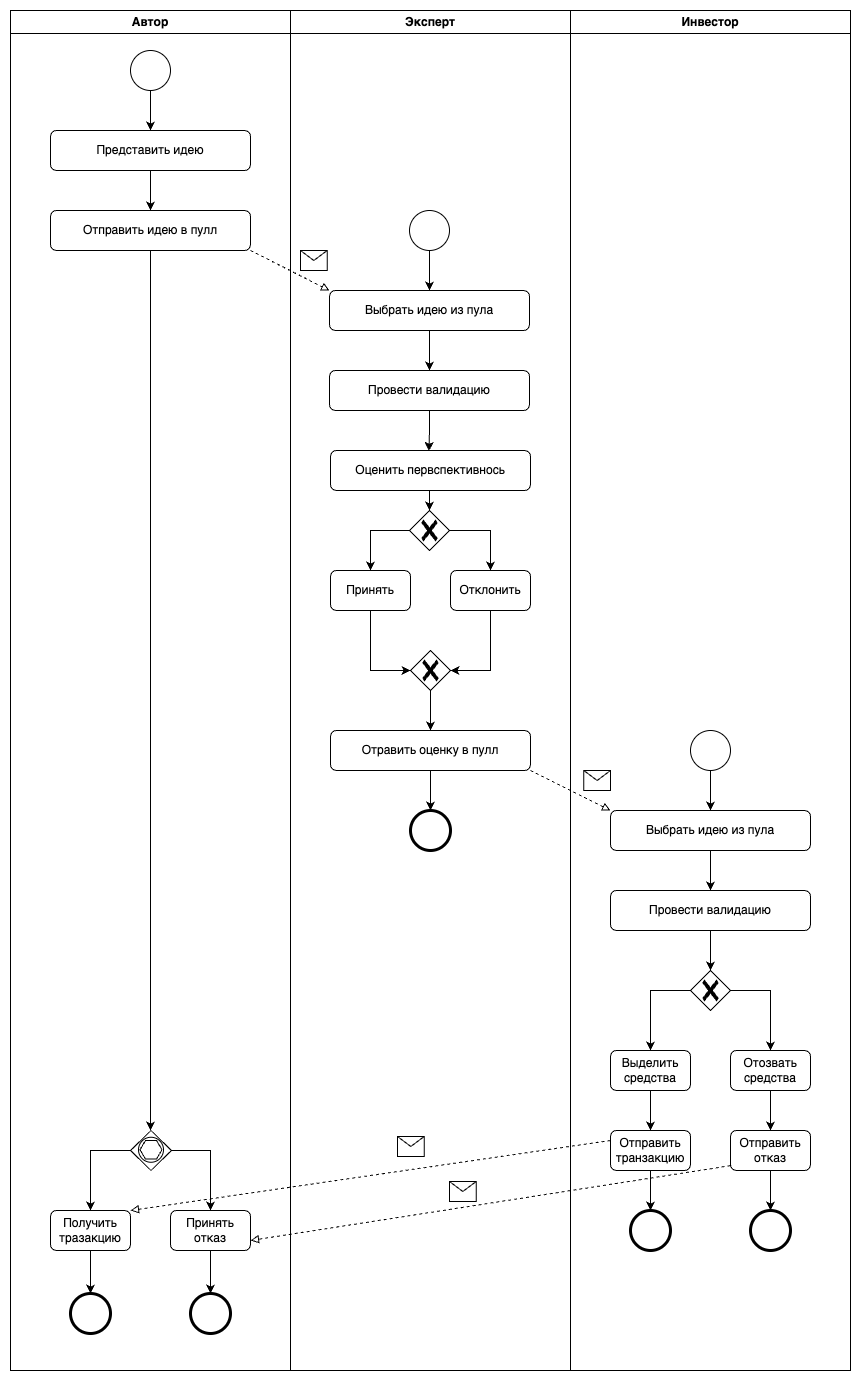
\includegraphics[width=0.5\textwidth]{./assets/bpmn.drawio.png}
  \caption{BPMN-диаграмма процессов масштабированного механизма инвестирования}
  \label{fig:bpmn}
\end{figure}

Информационное взаимодействие между пулом авторов и пулом экспертов осуществляется посредством асинхронных сообщений. В пуле экспертов активируется подпроцесс, включающий выбор идеи из общего пула, проведение валидации представленных данных и оценку перспективности проекта. Этот этап реализуется с применением искусственного интеллекта, который обрабатывает структурированные данные проекта с использованием ансамблевых методов машинного обучения. Диаграмма отражает ключевой шлюз (gateway) принятия решения, где эксперт формирует заключение о перспективности идеи на основе результатов аналитического движка и собственной экспертизы. Данное решение может иметь положительный или отрицательный характер, однако в обоих случаях процесс конвергирует к операции отправки оценки в общий пул, что завершает участие эксперта в текущем инвестиционном цикле.

Далее информационный поток направляется к пулу инвесторов, где инициируется подпроцесс выбора и независимой валидации идеи. Центральным элементом данного этапа является шлюз принятия инвестиционного решения, за которым следуют дивергентные пути процесса: выделение средств или отказ от инвестирования. В случае положительного решения активируется последовательность операций финансирования с использованием механизмов квадратичного финансирования и возрастающих кривых ограничения, реализованных посредством смарт-контрактов в выбранной блокчейн-инфраструктуре. При отрицательном решении формируется и отправляется уведомление об отказе.

Заключительный этап процесса визуализируется возвращением информационного потока к пулу автора, где происходит финальное разветвление процесса в зависимости от полученного результата: получение транзакции либо обработка отказа. Оба пути завершаются соответствующими конечными событиями, отражающими завершение инвестиционного цикла для конкретного проекта.

Особого внимания заслуживают интегрированные в диаграмму элементы, отражающие механизмы масштабирования платформы. Ethereum, что обеспечивает высокую пропускную способность системы при сохранении базового уровня безопасности. Данный подход позволяет поддерживать растущий объем транзакций без существенного увеличения операционных издержек, что критически важно для развития платформы. Параллельно отображаются процессы мониторинга производительности и автоматического масштабирования вычислительных ресурсов, обеспечивающие адаптивность системы к флуктуирующим нагрузкам.

Диаграмма также отражает ключевые подпроцессы, связанные с обеспечением безопасности и целостности данных, включая распределенное хранение зашифрованной информации в IPFS, применение мультисигнатурных механизмов для критических операций и регулярное резервное копирование состояния системы. Интеграция с внешними сервисами и API визуализируется посредством элементов сервисных задач, подчеркивая взаимодействие системы с внешними компонентами экосистемы.

В контексте управления процессом масштабирования значительную роль играют механизмы обратной связи, позволяющие оперативно корректировать параметры функционирования системы на основе получаемых метрик эффективности. Эти механизмы представлены на диаграмме в виде циклических потоков, соединяющих аналитические процессы с процессами принятия решений о параметрической оптимизации системы.

Таким образом, разработанная BPMN-диаграмма представляет собой комплексное формализованное описание функционирования масштабированного механизма инвестирования, интегрирующее как бизнес-логику взаимодействия ключевых участников, так и технологические аспекты, обеспечивающие масштабируемость, безопасность и адаптивность платформы в условиях возрастающей нагрузки и расширяющегося функционала.

\mysubsection{Формализация предметной области}

Пусть имеется конечный набор проектов \(P=\{p_{1},\dots ,p_{n}\}\) где
каждому проекту \(p_{i}\) требуется вложение капитала объёмом \(C_{i}\).
Также задано множество независимых участников \(A=\{a_{1},\dots ,a_{m}\}\).
Участник \(a_{j}\) может вложить сумму \(c_{ij}\ge 0\) в проект \(p_{i}\).
В ответ он получает выпущенные токены объёмом \(t_{ij}\), причём
\(t_{ij}\) пропорционален внесённому вкладу \(c_{ij}\).
Совокупный объём доступных для распределения средств обозначим через \(M\).

Задача механизма — распределить \(M\) так, чтобы максимизировать
суммарную выгоду участников системы, описываемую функцией
\(U\colon P\times A\to\mathbb{R}\), и одновременно  и одновременно гарантировать соблюдение принципов организации такой системы, изложенных в предыдущей главе. Экономический смысл такого механизма состоит в том, чтобы направлять ресурсы именно к тем проектам, чья ожидаемая общественная ценность максимальна, при этом балансируя интересы инвесторов и авторов проектов.


% ## 3.3
\mysection{Создание блокчейн среды}

Каждая стартап-идея токенизируется с использованием Augmented Bonding Curve (ABC), формирующей рыночную цену токена в зависимости от объёма эмиссии. Механизм Quadratic Funding (QF) усиливает проекты с широкой поддержкой, направляя дополнительное финансирование пропорционально квадрату сумм вложений. Инвесторы получают токены, которые автоматически блокируются до тех пор, пока рыночная цена не подтвердит их справедливую оценку, обеспечивая принцип skin-in-the-game.

\mysection{Классические венчурные инвестиции}

Венчурное инвестирование представляет собой форму финансирования инновационных проектов с высоким уровнем неопределённости и высоким потенциальным доходом. В отличие от долгового финансирования, венчурные инвестиции оформляются в виде обмена капитала на долю в компании, и возврат инвестиций возможен лишь при достижении компанией ликвидности — например, через выход на IPO, продажу (M\&A) или повторные инвестиционные раунды.

Одним из ключевых понятий в венчурной модели является оценка капитализации компании, то есть согласованное между сторонами представление о её будующей стоимости. Эта величина не всегда основана на текущих денежных потоках и может быть условной или завышенной при отсутствии рынка свободной торговли акциями. Наиболее распространённые механизмы инвестирования при которых инвестор предоставляет средства сейчас, а долю в компании получает в будущем — при наступлении определённых событий (например, следующем инвестиционном раунде).

Допустим, стартап получает инвестиции в размере $1$ миллиона долларов на условиях SAFE при post-money оценке $10$ миллионов. Это означает, что инвестор имеет право в будущем конвертировать свою инвестицию в 10\% долю компании. Основатели в этом случае фактически владеют 90\% компании, при этом важно отметить, что оценка является бумажной — на этом этапе акциями нельзя торговать, и их стоимость не гарантирована.

При успешном росте компании и последующих раундах, например на оценке в $100$ миллионов, доля раннего инвестора ($1$ миллион) увеличивается в абсолютном выражении в 10 раз. Это создаёт мощный стимул для рисковых инвестиций на ранней стадии. Однако если стартап сталкивается с трудностями, и вынужден привлекать капитал по более низкой оценке (down round), то доля основателей резко сокращается — из-за размывания (dilution).

Однако возникает опасность «раздутой» рыночной капитализации компании. Пример OpenAI, привлёкшего $40$ миллиардов при post-money оценке в $300$ миллиардов, иллюстрирует крайнюю форму позднего венчурного финансирования. В таких случаях компания фактически обязана добиться ликвидности на сопоставимом уровне — либо выйти на IPO, либо быть выкупленной с сохранением этой оценки. В противном случае возможна потеря капитала инвесторов и обнуление долей основателей, несмотря на теоретически высокую стоимость. \cite{}

Аналогичная ситуация возможна и в более ранних стадиях: при переоценке компании на $1$ миллиард и последующей продаже за $200$ миллионов стартап может оказаться в положении, когда все средства пойдут на покрытие обязательств перед инвесторами, а основатели и сотрудники, несмотря на многолетнюю работу, не получат ничего. В этом случае говорят о неустойчивом распределении риска, при котором high-valuation создает ложное ощущение устойчивости.

С точки зрения теории игр, классическая модель венчурного инвестирования опирается на допущение рациональности агентов и допуск высокой степени неопределённости. Однако, при неадекватных ожиданиях и отсутствии прибыльности, система теряет равновесие: инвесторы требуют экстренной ликвидности, стартап проводит раунды по заниженной оценке (down rounds), а команду приходится увольнять либо продавать компанию в ущерб долям всех предыдущих участников.

\begin{figure}[H]
  \centering
  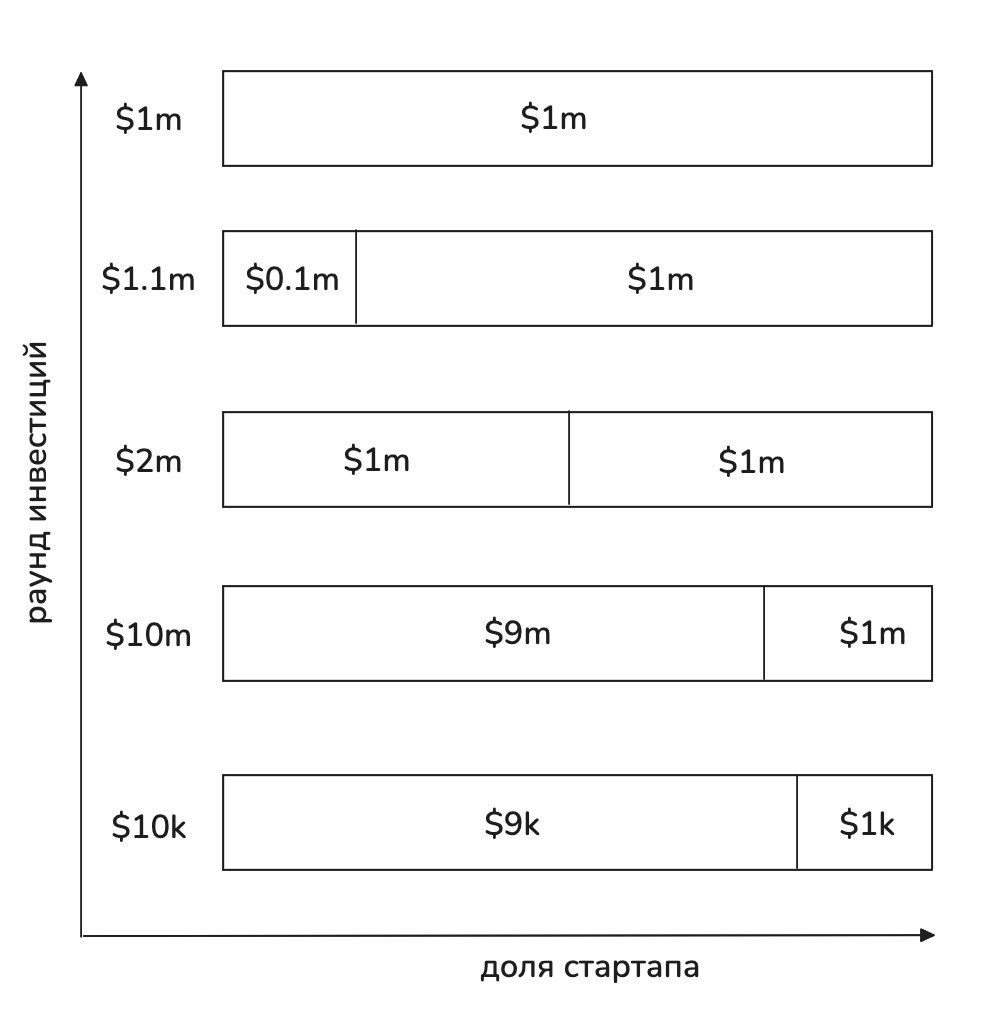
\includegraphics[width=0.6\textwidth]{./assets/investments.png}
  \caption{Схема оценки в классических венчурных инвестициях}
  \label{fig:investments}
\end{figure}


\mysubsection{Augmented Bonding Curve (ABC)}

Токенизацией через Augmented Bonding Curve (ABC) и механизмом Quadratic Funding (QF). Кривая ABC определяется формулой:
\[
  P(s) = \alpha \cdot s^\beta, \quad \beta = \frac{1}{1-r}, \quad r \in (0,1),
\]
где $s$ — текущее количество выпущенных токенов, $\alpha$ — масштабный коэффициент, а $r$ — резервный коэффициент. QF распределяет финансирование из общего пула на основе квадратичной функции индивидуальных вкладов:
\[
  M_i = \left(\sum_j \sqrt{c_{ij}}\right)^2,
\]
обеспечивая преимущество массовой поддержки над единичными крупными вкладами.

Для динамического ценообразования токена проекта $p_i$ используем
функцию
%
\[
  P_i(s)=\alpha_i\, s^{\beta_i}, \qquad
  \beta_i=\frac{1}{1-r_i}, \; r_i\in(0,1),
\]
%
где $s$~--- текущее количество выпущенных токенов.
При вкладе $c_{ij}$ инвестор $a_j$ получает
\[
  t_{ij} \;=\; \frac{c_{ij}}{P_i\!\bigl(s_{\text{prev}}\bigr)},
\]
что уточняет ранее введённое условие пропорциональности
$t_{ij}\propto c_{ij}$.
Таким образом, ABC связывает размер выпуска с резервом
и делает цену токена функцией совокупного предложения
\cite{Zargham2019}.

Реализация контракт ERC‑20 с автоматическим ценообразованием по кривой \ref{lst:abc}
\begin{lstlisting}[language=Solidity, caption={Пример реализации ERC-20 с ABC}, label={lst:abc}]
contract ABCToken is ERC20, Ownable {
    uint256 public alpha;  // масштабный коэффициент
    uint256 public reserveRatio; // резервный коэффициент r
    uint256 public totalSupply;
    uint256 public reserveBalance;

    event TokensMinted(address indexed to, uint256 amount, uint256 price);
    event TokensBurned(address indexed from, uint256 amount, uint256 price);

    constructor(
        string memory name,
        string memory symbol,
        uint256 _alpha,
        uint256 _reserveRatio
    ) ERC20(name, symbol) {
        require(_reserveRatio > 0 && _reserveRatio < 1e18, "Invalid reserve ratio");
        alpha = _alpha;
        reserveRatio = _reserveRatio;
    }

    function calculatePrice(uint256 supply) public view returns (uint256) {
        // P(s) = a * s^B, где B = 1/(1-r)
        uint256 beta = 1e18 / (1e18 - reserveRatio);
        return alpha * (supply ** beta) / 1e18;
    }

    function buyTokens() external payable {
        require(msg.value > 0, "Must send ETH");

        uint256 currentPrice = calculatePrice(totalSupply);
        uint256 tokensToMint = (msg.value * 1e18) / currentPrice;

        _mint(msg.sender, tokensToMint);
        reserveBalance += msg.value;
        totalSupply += tokensToMint;

        emit TokensMinted(msg.sender, tokensToMint, currentPrice);
    }

    function sellTokens(uint256 amount) external {
        require(amount > 0, "Amount must be positive");
        require(balanceOf(msg.sender) >= amount, "Insufficient balance");

        uint256 currentPrice = calculatePrice(totalSupply - amount);
        uint256 ethToReturn = (amount * currentPrice) / 1e18;

        require(reserveBalance >= ethToReturn, "Insufficient reserve");

        _burn(msg.sender, amount);
        reserveBalance -= ethToReturn;
        totalSupply -= amount;

        payable(msg.sender).transfer(ethToReturn);

        emit TokensBurned(msg.sender, amount, currentPrice);
    }

    function getCurrentPrice() external view returns (uint256) {
        return calculatePrice(totalSupply);
    }
}
\end{lstlisting}

% 3.2.2
\mysubsection{Блокировака активов}

Происходит локинг токенов через обратную ABC-кривую до тех пор, пока они не достигнут "справедливой цены" или пока рынок не выночную стоимось.

В классической экономике спрос и предложение определяют цену актива. При высоком спросе и ограниченном предложении цена возрастает, при избыточном предложении и сниженном спросе — снижается. Аналогичная логика применяется к токенам в системе ABC: если токены активно приобретаются, цена растёт. Однако в предложенной модели продажа токенов ограничивается, пока рынок не подтвердит их оценку.

Механизм реализуется следующим образом:
\begin{enumerate}
  \item При покупке токена по текущей цене $P(s)$ создаётся запись о цене приобретения $P_{\text{buy}}$.
  \item Полученные токены блокируются и не подлежат выводу до выполнения одного из двух условий:
        \begin{itemize}
          \item Рыночная цена $P_{\text{now}} \geq P_{\text{buy}}$;
          \item Истечение установленного времени $L$.
        \end{itemize}
  \item Таким образом, вывод токенов становится возможным только при подтверждённой устойчивости их оценки либо по завершении установленного локапа.
\end{enumerate}

Если предложение обогнало спрос перекуплен,  раздут, цена токена должна упасть — но ABC этого не допускает и цена всегда растет.

Поэтому мы блокируем токены и не даёшь продать их, пока система не уверена, что спрос подтвердил valuation.

Код блокирования активов представлен в листинге \ref{lst:locker}.

\begin{lstlisting}[language=Solidity, caption={Пример реализации смарт контракта для блокирования активов}, label={lst:locker}]
contract TokenLocker {
  mapping(address => uint256) public lockedBalances;
  mapping(address => uint256) public lockedTimestamps;

  function lockTokens(uint256 amount, uint256 price) public {
    lockedBalances[msg.sender] += amount;
    lockedTimestamps[msg.sender] = block.timestamp;
    lockedPrices[msg.sender] = price;
  }
}
\end{lstlisting}

% 3.2.3
\mysubsection{Quadratic Funding (QF)}

Механизм отражает поведение на венчурном рынке, где стартапы последовательно привлекают инвестиции, увеличивая оценку (valuation). Если проект не демонстрирует подтверждённого роста, а оценка оказывается завышенной, дальнейшее финансирование невозможно без снижения valuation, что может привести к невозможности выхода инвесторов и гибели компании. Аналогично, если токен в системе не демонстрирует дальнейшего спроса, резервные фонды истощаются, а цена перестаёт расти, инвестиции остаются заблокированными до изменения рыночной ситуации.

Софинансирование из общего пула $M$ определяется правилом
\[
  M_i \;=\; \Bigl(\sum_{j}\sqrt{c_{ij}}\Bigr)^2
  \quad\Longrightarrow\quad
  \tilde{C}_i \;=\; \sum_{j} c_{ij}+M_i ,
\]
где $\tilde{C}_i$~--- эффективный объём капитала проекта.
QF изменяет целевую функцию полезности:
\[
  U(p_i,A)\;\longrightarrow\;
  U^{\text{QF}}(p_i,A)
  \,=\,U\!\bigl(\tilde{C}_i,A\bigr),
\]
усиливая влияние массовой поддержки

В результате мы получаем систему, где инвесторы получают токены, которые автоматически блокируются до тех пор, пока рыночная цена не подтвердит их справедливую оценку.

Код механизма QF представлен в листинге \ref{lst:qf}.

\begin{lstlisting}[language=Solidity, caption={Пример реализации смарт контракта для механизма QF}, label={lst:qf}]
contract QuadraticFunding {
  mapping(address => uint256) public contributions;
  uint256 public totalContributions;
  uint256 public totalFunds;

  function contribute(uint256 amount) public {
    contributions[msg.sender] += amount;
    totalContributions += amount;
    totalFunds += amount;
  }
}
\end{lstlisting}

% ## 3.3 Агент
\mysection{Участники системы}

Адаптация параметров механизма во времени реализована отдельным компонентом, который может быть офф-чейн скриптом или сервисом, взаимодействующим с блокчейном. Он периодически собирает данные о системе (объем инвестиций, количество участников, частоту отклоняющихся голосов, случаи потерь stake, волатильность цены токена и т.д.), обновляет состояние для модели и принимает решение, нужно ли скорректировать параметры $\alpha, r, \tau, L$ или размер вознаграждений/штрафов. Такой модуль можно рассматривать как агента, действующего в среде, состояние которой – это текущее состояние платформы, а действия – это установка новых значений параметров. Цель агента – максимизировать некоторый кумулятивный рейтинговый показатель $R_t$ системы (например, метрику устойчивости и эффективности). Мы можем задать задачу как поиск оптимальной политики $\pi^*$, выбирающей действие $a_t$ (набор параметров) на каждом шаге $t$, чтобы максимизировать дисконтированную сумму наград $\sum \gamma^t R_t$ с коэффициентом дисконтирования $0<\gamma<1$. Формально, агент решает задачу оптимизации:

\[
  \pi^* = \arg \max_{\pi} E_{\pi} \left[ \sum_{t=0}^{\infty} \gamma^t R_t \right],
\]

% ## 3.3.1
\mysubsection{Proof of Stake (PoS)}

Основной уязвимостью QF являются Sybil-атаки, устранение которых реализовано по аналогии с помощью механизма proof of stake \cite{Hansson2000} создающим экономический барьер для многочисленных фейковых аккаунтов.

Каждый валидатор вкладывает залог $s_j$.
Обновление залога по итогам раунда оценки задаётся правилом
\[
  s_j' \;=\;
  \begin{cases}
    s_j(1+\rho),   & \text{прогноз верен},   \\[4pt]
    s_j(1-\sigma), & \text{прогноз неверен},
  \end{cases}
\]
где $\rho\ge 0$ и $0\le\sigma\le 1$.
Потенциальный штраф $\sigma s_j$ вводит
стоимость Sybil-атаки и
модифицирует индивидуальную полезность агента:
\[
  U_j^{\text{PoS}}
  \,=\,U_j-\sigma s_j .
\]
Тем самым PoS защищает формулу распределения средств
от манипуляций со стороны агентов \cite{Kiayias2017}.

Согласно теории игр, описанный механизм приводит систему к динамическому равновесию Нэша \cite{nash1951non}, в котором ни одному агенту не выгодно отклоняться от честного поведения. Каждый агент ставит часть капитала (stake), рискуя им при оценке проекта. Если его прогноз согласуется с коллективным результатом, ставка возвращается с прибылью, иначе частично или полностью теряется. Таким образом, рациональный агент мотивирован действовать честно и использовать всю доступную ему информацию.

В разработанной системе децентрализованного распределения инвестиций устойчивость достигается благодаря тому, что честное поведение каждого агента становится рациональной и доминирующей стратегией. Данное свойство можно формально описать через равновесие Нэша, при котором ни одному участнику не выгодно отклоняться от стратегии честного взаимодействия, если остальные участники придерживаются её же.

Каждый агент может выбирать между стратегией добросовестного участия — инвестируя в проект, который он считает перспективным, на собственное имя и с риском получения или потери прибыли — и стратегией манипуляции, например, попыткой раздробить вклад на несколько адресов (Sybil-атака) с целью искусственно усилить значение квадратичного сигнала QF и тем самым получить непропорционально большую долю софинансирования. Однако механизм PoS, встроенный в систему, предусматривает, что итоговая полезность агента напрямую зависит от успеха оценённого им проекта. В случае некорректной оценки, независимо от числа Sybil-адресов, каждый из них несёт риск потери вложенного капитала, пропорционально его размеру. При этом срабатывает обратная зависимость: дробление увеличивает вероятность ошибки и масштаб потенциальных потерь, поскольку каждый поддельный адрес оценивается отдельно и подвержен штрафу.

\begin{figure}[H]
  \centering
  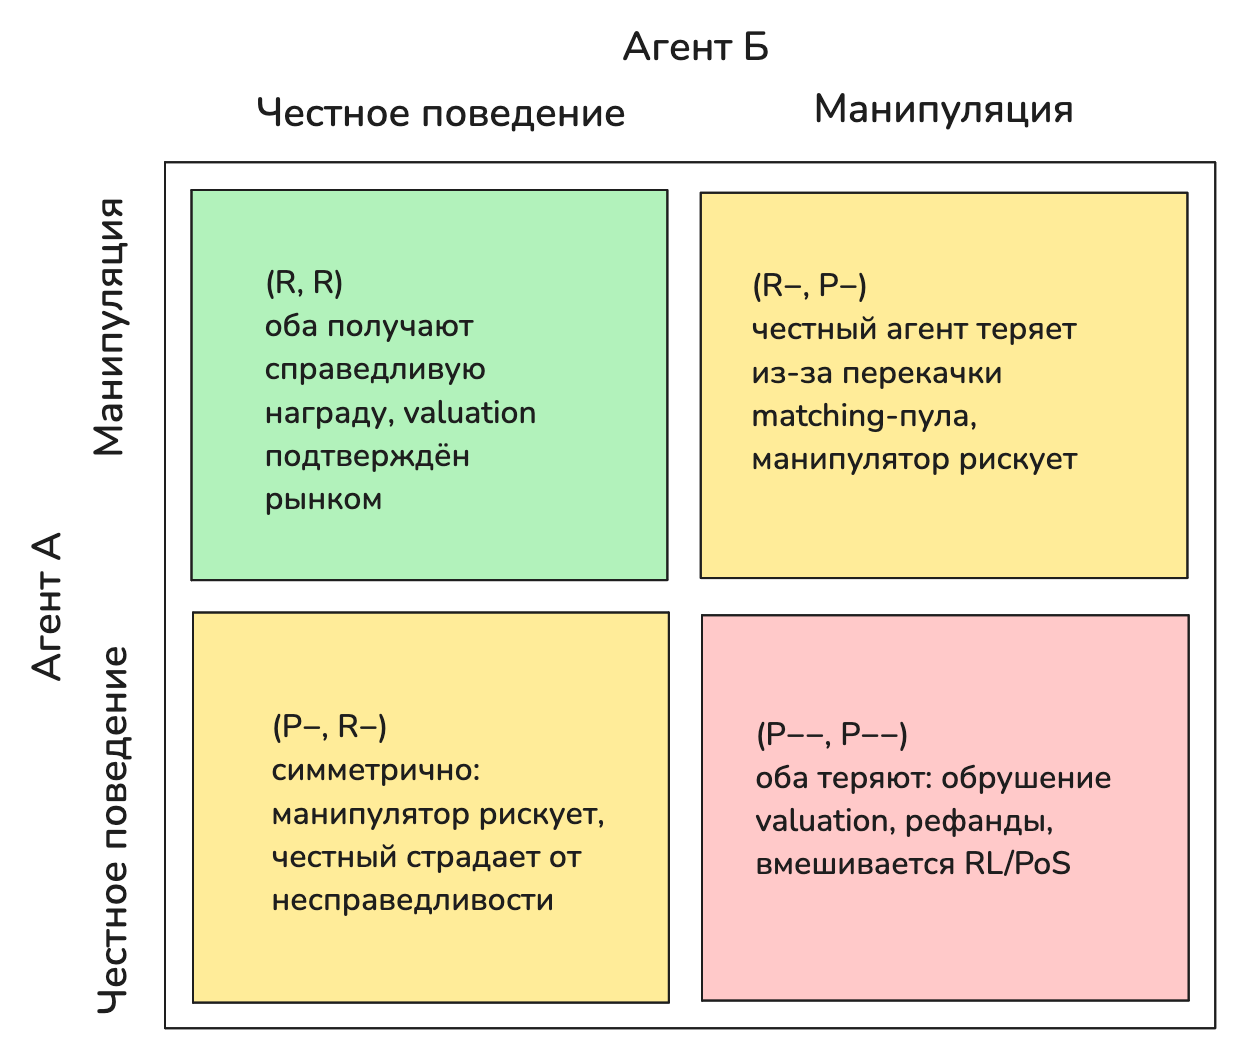
\includegraphics[width=0.5\textwidth]{./assets/nash-equilibrium.png}
  \caption{Равновесие Нэша}
  \label{fig:nash-equilibrium}
\end{figure}

Анализ стратегий показывает, что при честном поведении обоих участников ни один из них не получает стимулов к отклонению: система работает устойчиво, токены разблокируются по мере подтверждения оценки со стороны рынка, а valuation проекта отражает реальный спрос. Если один из участников пытается манипулировать, результатом становится временное преимущество, сопровождаемое повышенным риском блокировки токенов, срабатыванием PoS-механизма, корректировкой параметров токеномики через RL-модель, и в итоге — снижением ожидаемой прибыли. При одновременном нечестном поведении всех агентов система сталкивается с резким падением доверия, инфляцией оценки, массовыми попытками рефанда и активацией защитных мер: повышение резервных коэффициентов, увеличение длительности локинга и снижение эффективности QF. Таким образом, равновесие Нэша достигается за счёт того, что для любого отдельного агента честное поведение остаётся оптимальной стратегией независимо от выбора остальных.

Индивидуальному агенту не выгодно нарушать правила, и выгодно совершать полезную работу по оценке стартапов (предсказывать). В системе честное поведение становится доминирующей стратегией для каждого агента.

\mysubsection{Устойчивость системы}

Предположим, что злонамеренный агент $a_j$ намеренно стремится обмануть систему, например, раздувая оценку проектов через раздробленные вложения, искажая сигналы Quadratic Funding (QF), или манипулируя рыночным ожиданием через искусственный рост объёма транзакций. Однако в описанном механизме каждый агент связан не только с возможностью получения прибыли, но и с экономическими рисками, встроенными в архитектуру системы, которые делают подобные атаки невыгодными при рациональном анализе.

Этот принцип был впервые формализован в работе \cite{nakamoto2008bitcoin}, где доказывается, что индивидуальному участнику распределённой системы, в которой вознаграждение напрямую зависит от общего состояния цепи и синхронного консенсуса, невыгодно действовать против правил: любые попытки отклонения требуют вложений, которые могут не окупиться, а при равном или меньшем вычислительном (или экономическом) весе — попросту теряются.

\begin{figure}[H]
  \centering
  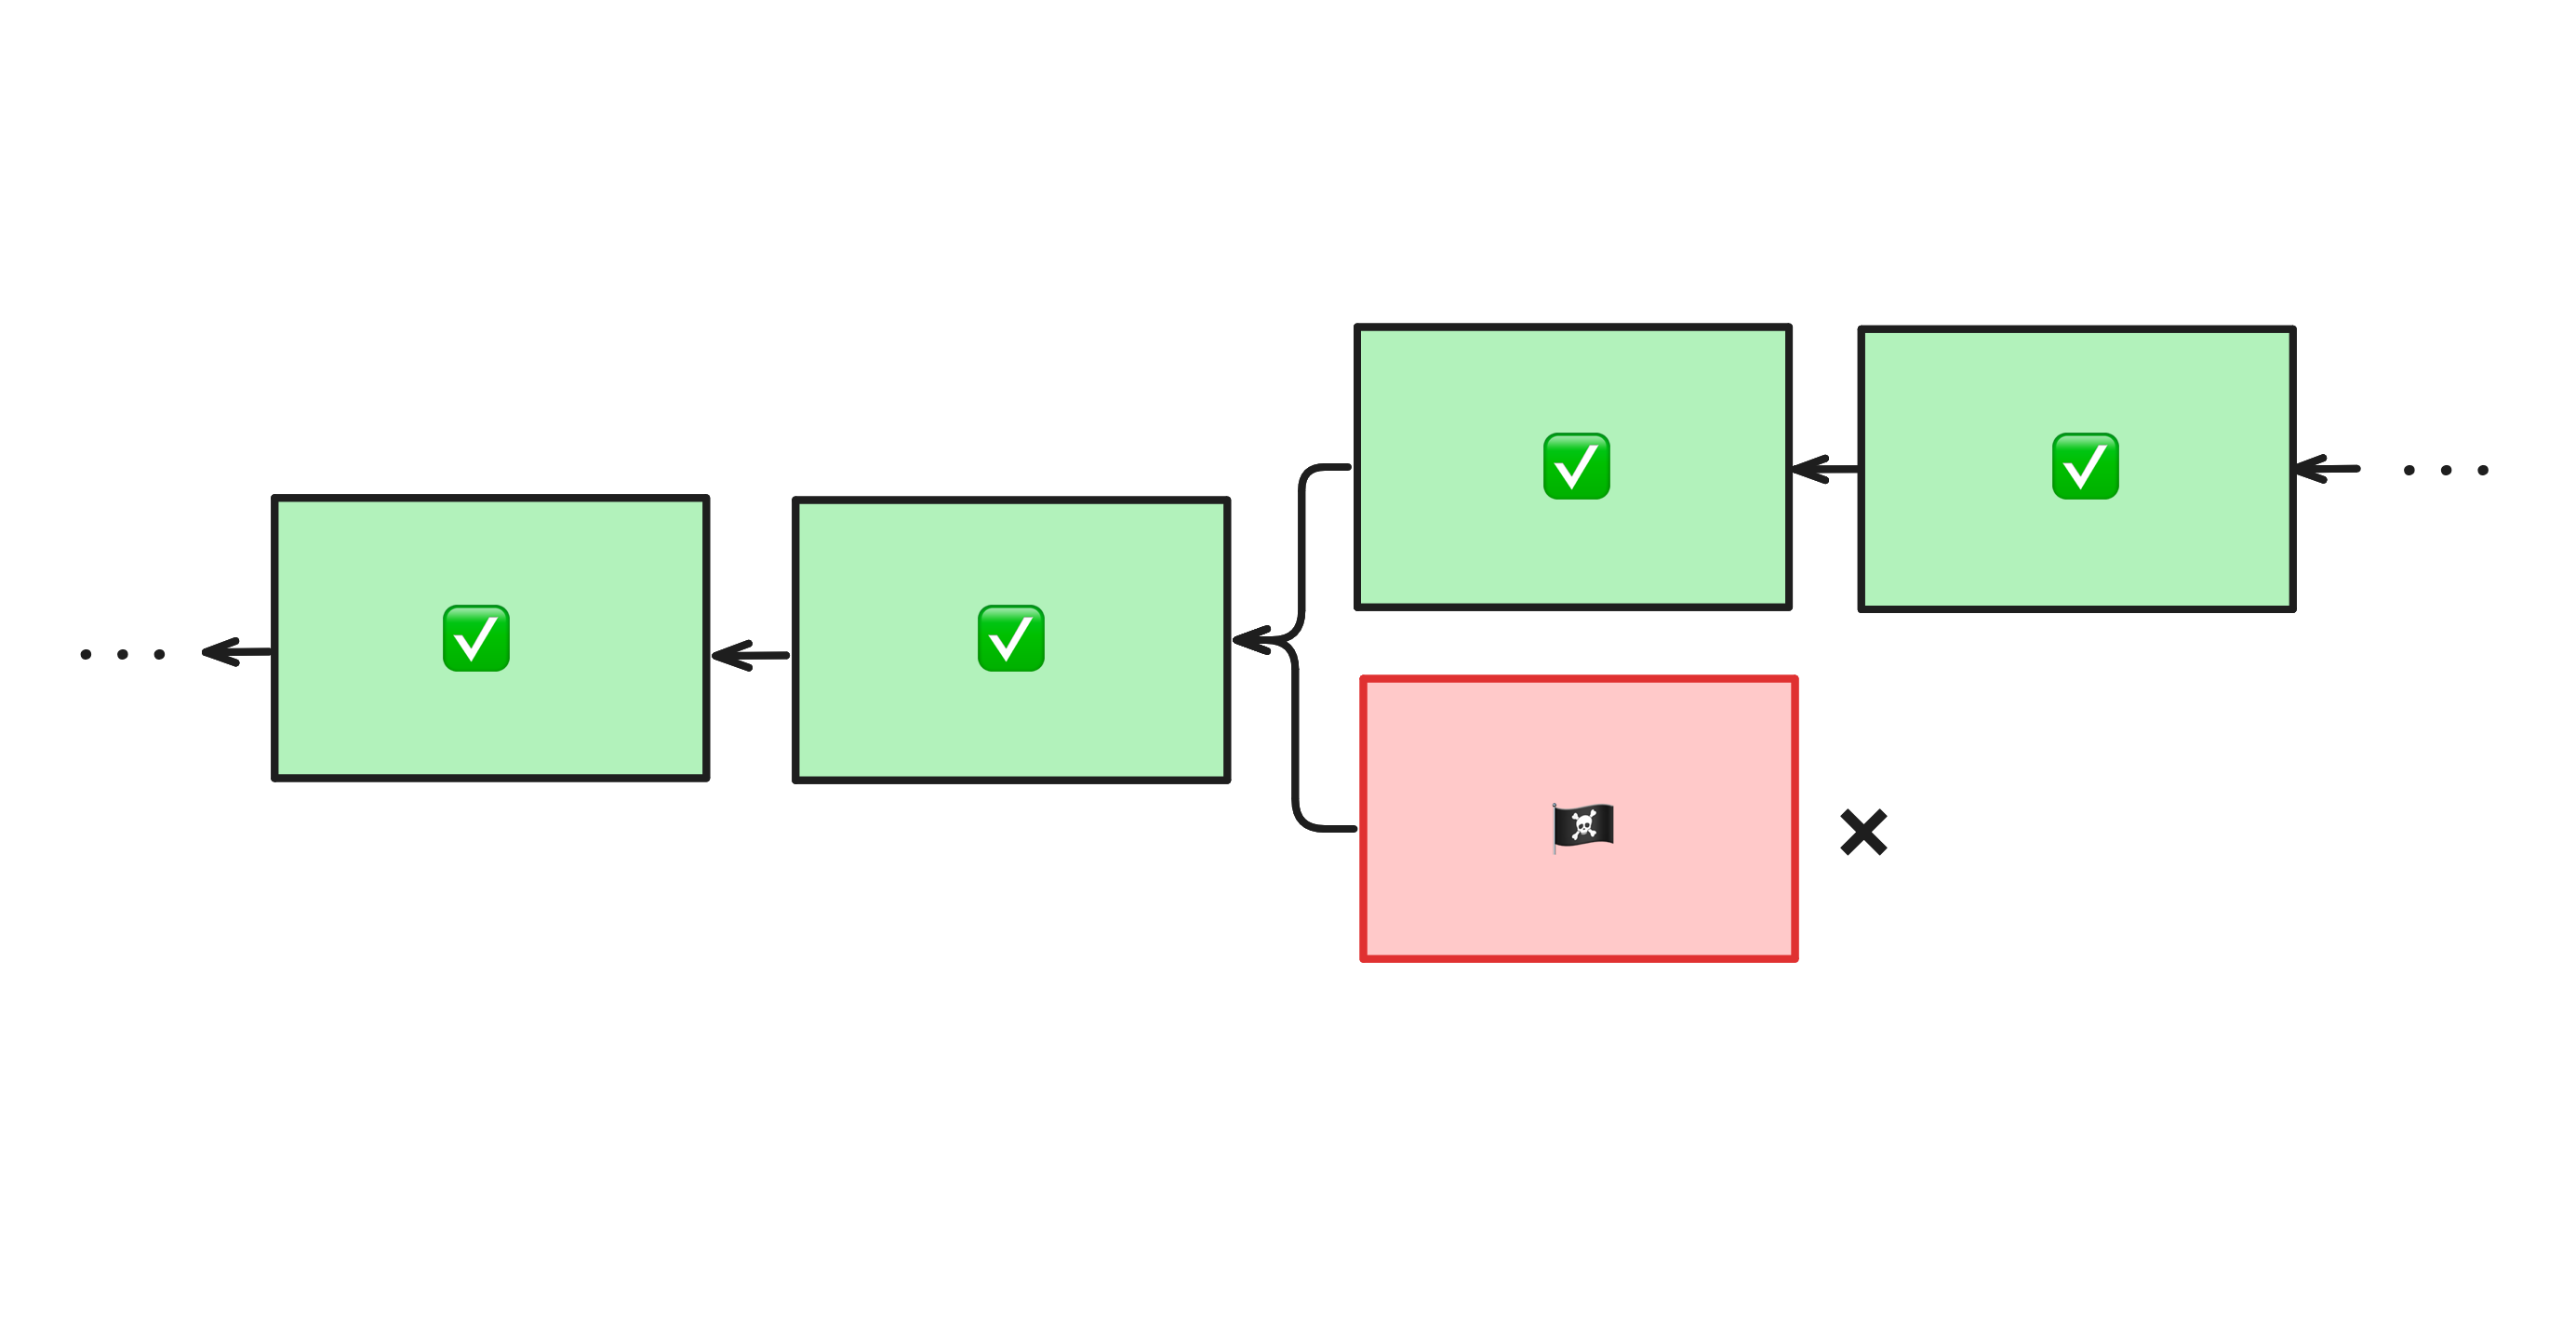
\includegraphics[width=0.9\textwidth]{./assets/longest-chain.png}
  \caption{Индивидуальному пользователю не выгодно пытаться обмануть систему, поскольку она всегда следует наиболее «длинной» (то есть экономически выгодной и честной) цепочке действий.}
  \label{fig:longest-chain}
\end{figure}

Для защиты от искажений, система использует механизм Proof of Stake (PoS) \cite{king2012ppcoin}, в котором каждый агент рискует собственным капиталом. При этом stake в данной модели — это не отдельный залог, а вложение в проект, результат которого служит источником истины: если проект оказался переоценённым и в дальнейшем не подтвердил ожиданий (например, через падение цены токена, отказ от выкупа или негативную валидацию), агент теряет часть своего первоначального вклада. Таким образом, всякий некорректный прогноз или манипулятивное поведение автоматически наказывается экономически, без необходимости ручной модерации.

% ## 3.4 Механизм
\mysection{Создание нейросетевой модели}

Хотя описанная в предидущем пункте система является достаточно устойчивой, она может быть улучшена за счет применения нейросетевой модели, которая будет регулировать параметры системы в зависимости от экономических условий. Инфляция и дефляция в экономических системах являются результатом нарушения баланса между совокупным спросом и доступным объёмом ценности в обращении. В условиях, когда поведение агентов определяется локальными стимулами, а общая картина взаимодействий недоступна каждому участнику, малые отклонения могут приводить к системным эффектам. Инфляция возникает при росте объёма инвестиций или спроса, который не сопровождается соответствующим увеличением реальной ценности — это приводит к перегреву: цена актива растёт, не будучи обеспеченной фундаментальными показателями. Напротив, дефляция наблюдается, когда активы обесцениваются из-за снижения спроса, утраты доверия или стремления агентов к ликвидности, что запускает самоподдерживающийся нисходящий процесс.

Обе ситуации связаны с эффектами обратной связи: положительной — в случае инфляции, когда рост цен провоцирует дополнительный спрос, и отрицательной — в случае дефляции, когда снижение стоимости усиливает отток. Без регулирующего механизма, способного адаптивно изменять параметры среды и сдерживать экстремальные отклонения, система утрачивает способность к устойчивому равновесию, даже если каждый агент действует рационально в отдельности. Таким образом, устойчивость требует не только внутренней экономической логики, но и уровня координации, способного сглаживать флуктуации и восстанавливать баланс между локальными действиями и глобальной динамикой.

% ### 3.4.1
\mysubsection{Экономический дисбаланс}

Предположим, что в системе возникает локальный или глобальный экономический дисбаланс: например, при массовом росте числа проектов, каждый из которых требует привлечения средств, совокупного объёма доступных инвестиций может оказаться недостаточно. Это приведёт к снижению эффективности токенизации (механизм ABC перестаёт наполняться ликвидностью), а сами стартапы не смогут получить необходимый уровень софинансирования, несмотря на наличие поддержки со стороны сообщества. При обратной ситуации — если в систему в короткий период поступает чрезмерно большой объём инвестиций, но количество актуальных проектов остаётся ограниченным, — происходит перегрев оценки. Проекты получают завышенный объём средств до достижения рыночного подтверждения (traction), что стимулирует спекулятивное поведение и инфляцию стоимости токенов без реального роста фундаментальных показателей.

Таким образом, система потенциально уязвима как к дефициту капитала (дефляция), так и к избыточному спросу (инфляция), каждый из которых разрушает экономические стимулы — либо снижая доверие к системе (если проекты не получают нужной поддержки), либо девальвируя награду инвестора (если valuation оказывается несостоятельной).

Для предотвращения этих эффектов в системе применяется нейросетевая RL-модель, выступающая в роли макроэкономического регулятора.

Пример работы механизма управления представлен на рисунке \ref{fig:rl-example}.

\begin{figure}[H]
  \centering
  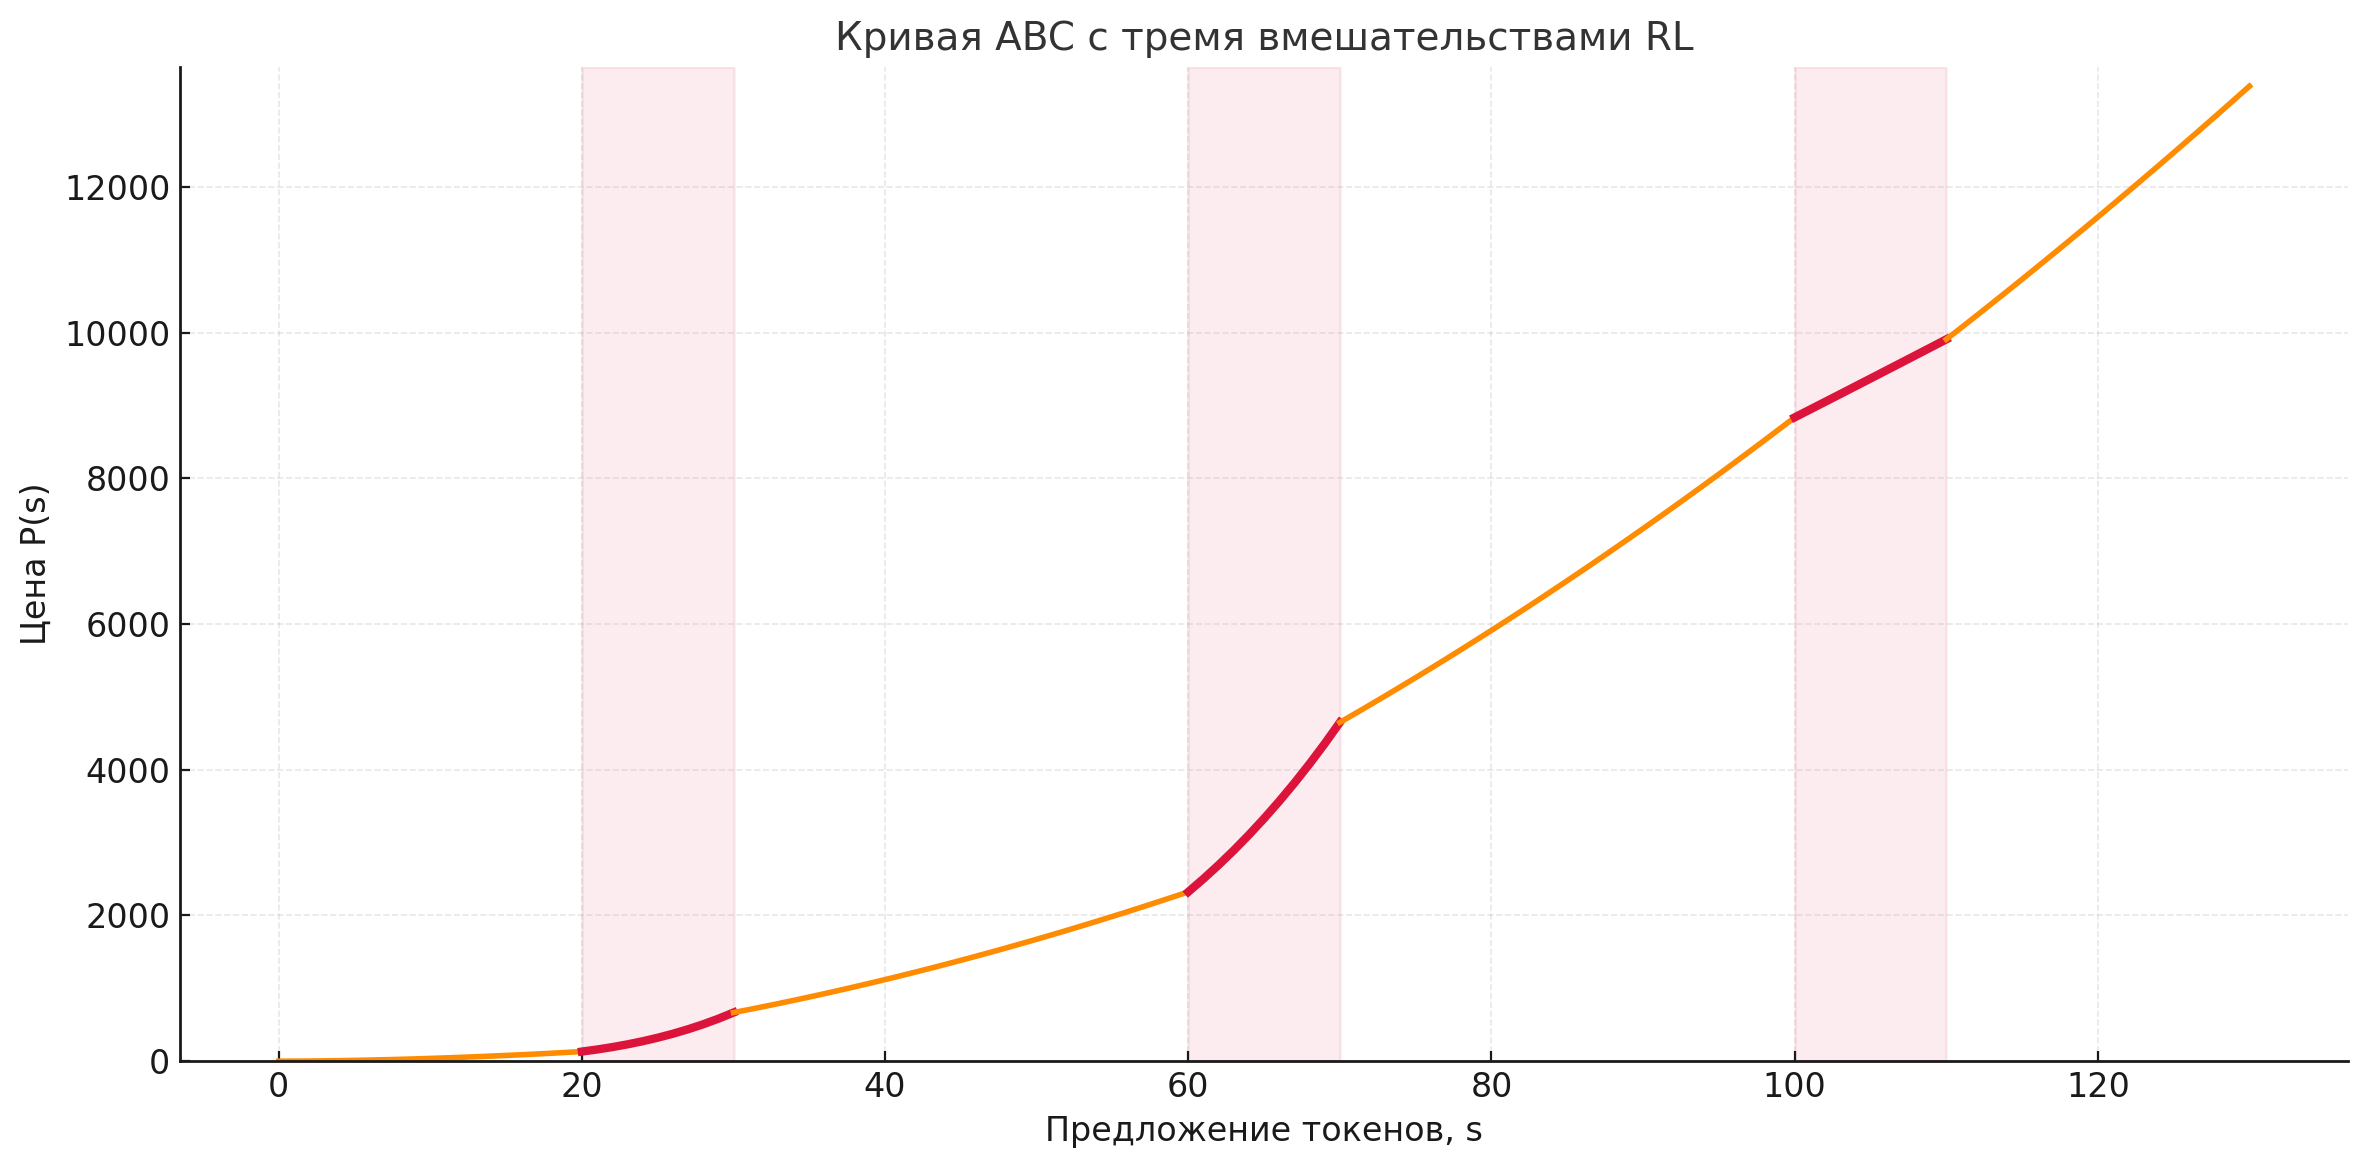
\includegraphics[width=0.9\textwidth]{./assets/rl-example.png}
  \caption{Иллюстрацию механизма ABC+QF с примерами распределения финансирования.}
  \label{fig:rl-example}
\end{figure}

Целью модели является удержание системы в экономически устойчивом диапазоне, при котором одновременно соблюдаются интересы двух ключевых групп: авторов проектов, получающих финансирование и инвесторов, заинтересованных в возврате и росте стоимости вложений.

Состояние среды включает в себя параметры, отражающие текущий экономический климат: общий объём инвестиций, динамику количества активных проектов, волатильность токенов, частоту возвратов и скорость выкупа.

Для механизма управления была выбрана нейросетеая RL модель, которая служит для изменения параметров системы целиком балансируя тем самым интересы проектов и инвесторов. Она в роли центрального регулятора системы, аналогично центральному банку, и оптимизирует только общие для всех параметры кривой роста капитализации проектов в системе.

% ### 3.4.2
\mysubsection{RL модель распределения ресурсов}

Алгоритм RL рассматривает состояние
$s_t=\bigl(\alpha_i,r_i,\tilde{C}_i,\text{метрики поведения}\bigr)$
и выбирает действие
$a_t=\bigl(\Delta\alpha_i,\Delta r_i,\Delta\tau_i,\Delta L_i\bigr)$,
обновляя параметры ABC и сопутствующие коэффициенты:
\[
  (\alpha_i,r_i,\tau_i,L_i)\;\gets\;(\alpha_i,r_i,\tau_i,L_i)+a_t .
\]
Оптимальную стратегию
\(
\pi^*=\arg\max_\pi\mathbb{E}_\pi
\bigl[\sum_{t}\gamma^t R_t\bigr]
\)
обучаем так, чтобы величина $R_t$ отражала рост
$U^{\text{QF}}(p_i,A)$ и снижение числа нарушений,
что адаптивно корректирует саму формулу $P_i(s)$
и связанное с ней распределение токенов.

Таким образом, RL действует как экономический регулятор, ограничивая раздувание оценки без подтверждения рыночного интереса и защищая долгосрочные интересы как инвесторов, так и инициаторов проектов.

Для решения этой задачи применяется алгоритм обучения с подкреплением. Для обучения был выбран метод deep-Q network, так как в системе необходим глубокий анализ поведения агентов. Ниже приведён код на Python, демонстрирующий использование библиотеки Stable-Baselines3 для обучения RL-агента в среде проекта (см. листинг~\ref{lst:rlmodel}).

\begin{lstlisting}[language=Python, caption={Пример кода RL-агента}, label={lst:rlmodel}]
import gym
from stable_baselines3 import PPO

class MechanismEnv(gym.Env):
    def __init__(self, initial_params):
        super().__init__()
        self.observation_space = gym.spaces.Box(low=0, high=1, shape=(N,), dtype=float)
        self.action_space      = gym.spaces.Box(low=0, high=1, shape=(4,), dtype=float)
        self.state = self._get_state_from_params(initial_params)

    def step(self, action):
        new_params = self._action_to_params(action)
        self._apply_params(new_params)
        outcome = simulate_round(new_params)
        reward = outcome["utility"] - outcome["penalty"]
        self.state = self._get_state_from_params(new_params)
        done = False
        return self.state, reward, done, {}

    def reset(self):
        self.state = self._get_state_from_params(initial_params)
        return self.state

env = MechanismEnv(initial_params={"alpha": 1.0, "r": 0.5, "tau": 0.1, "L": 30})
model = PPO("MlpPolicy", env, verbose=1)
model.learn(total_timesteps=100000)
optimal_params = model.policy.predict(env.state)
print("Optimal parameters found:", optimal_params)

\end{lstlisting}

% ### 3.4.3
\mysubsection{Анализ резаультатов работы модели}

Данный алгоритм был протестирован на смоделированной выборке из DEX и показал хорошие результаты на 500 эпохах.

\begin{figure}[H]
  \centering
  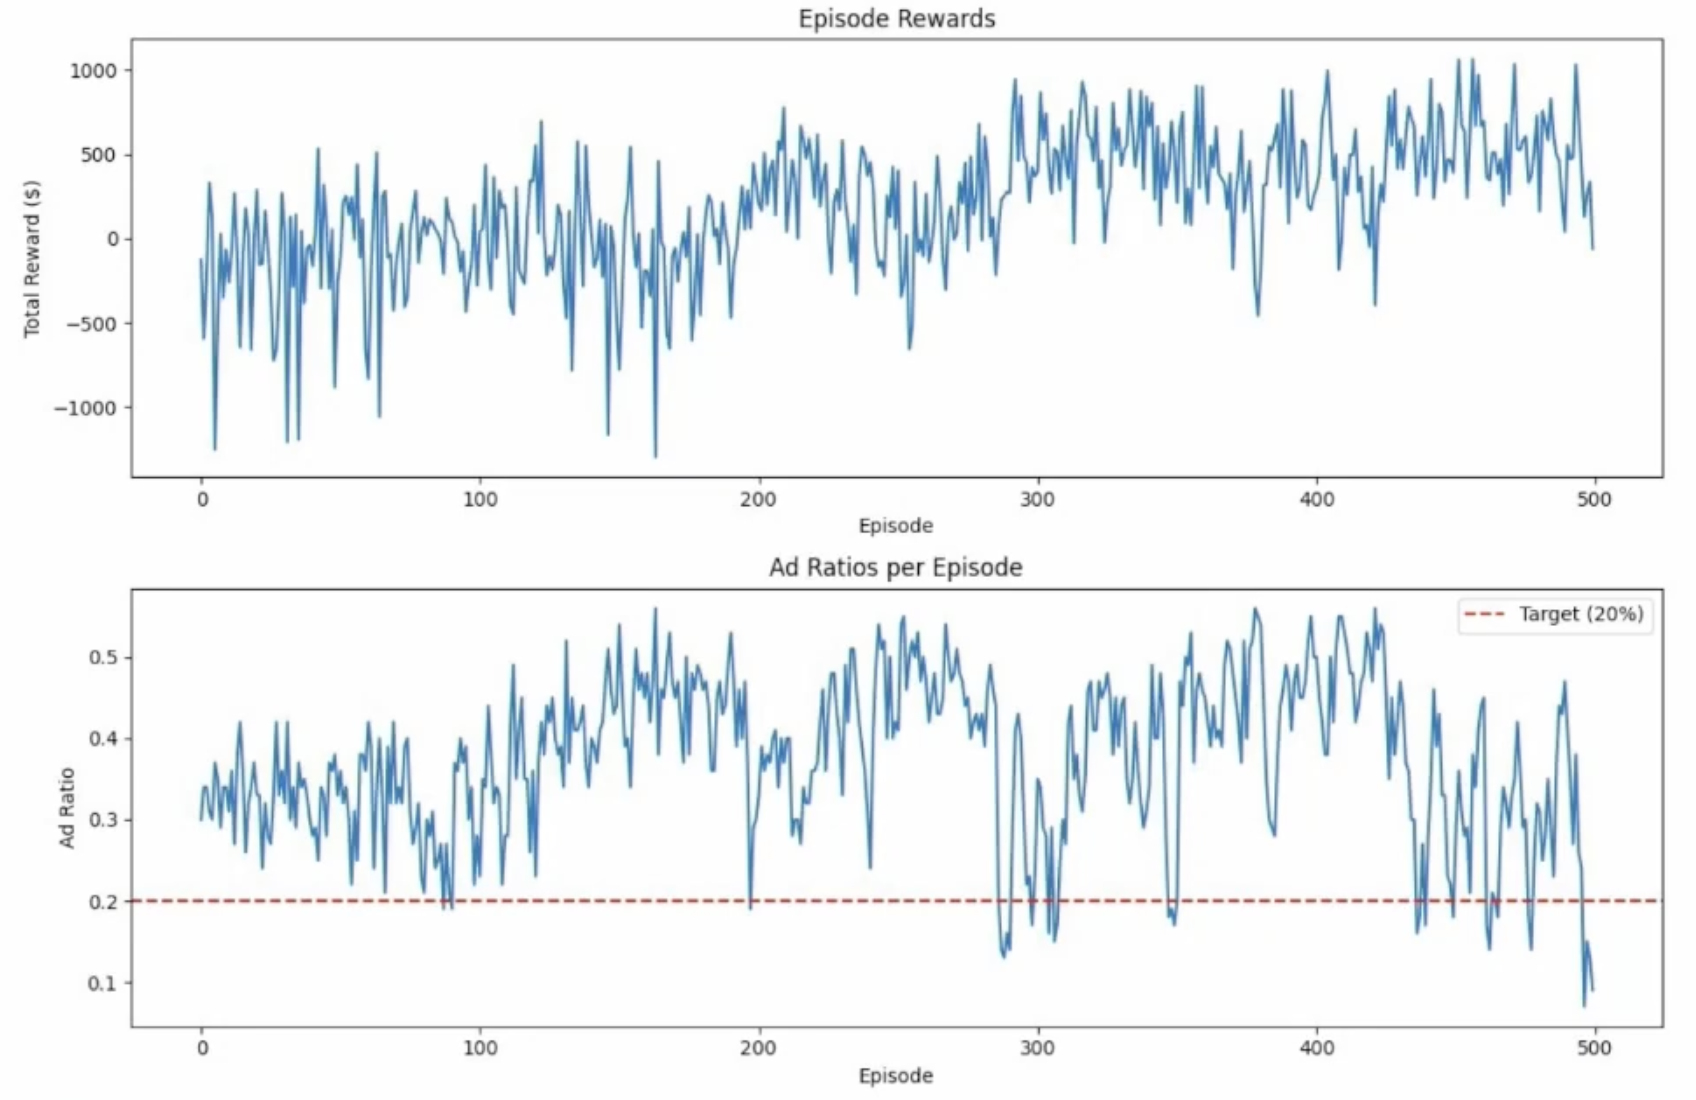
\includegraphics[width=0.9\textwidth]{./assets/q-network.png}
  \caption{Результаты работы QDN}
  \label{fig:rl-model}
\end{figure}

% ## 3.5
\mysection{Вывод по третей главе}

Таким образом, разработан механизм, сочетающий стимулы, рациональность агентов и доверенный механизм согласования, что позволяет эффективно распределять ресурсы на основе коллективных прогнозов.

С практической стороны инвесторы предоставляют ликвидность авторам стартапов, которые в зависимости от результата проекта могут выкупать токены полностью, частично или не выкупать совсем. Инвесторы защищены механизмом возврата инвестиций при провале проекта.

% ###################################################
% # Глава 4
\mychapter{РАЗРАБОТКА ДЕЦЕНТРАЛИЗОВАННОГО ПРИЛОЖЕНИЯ}
% ###################################################

Глава содержит описание архитектуры, бизнес-процессов, технических решений и реализации прототипа платформы для коллективного инвестирования.

% ## 4.1
\mysection{Архитектура платформы и основные компоненты}

Архитектура платформы построена с учётом принципов децентрализации и отказоустойчивости. Основу архитектуры составляют несколько модулей, функционирующих независимо, но взаимосвязанных через интерфейсы и стандартизированные протоколы. Модульность позволяет каждой компоненте развиваться автономно, без существенного влияния на общую работу платформы. Центральной частью архитектуры является слой блокчейна. Данная архитектура построена на модульном принципе, когда различные компоненты, оставаясь взаимосвязанными, функционируют независимо, что обеспечивает гибкость системы и возможность эволюционного развития отдельных её частей. В основе проектирования лежит идея распределения критически важных данных и сервисов по сети, что устраняет единую точку отказа и позволяет обеспечить устойчивость к цензуре, а также применение криптографических методов и принципа минимального необходимого доступа, что гарантирует безопасность и защиту конфиденциальной информации. Архитектура приложения представляет собой распределенную систему, включающую фронтенд, бэкенд и вспомогательные сервисы, разворачиваемые посредством CI/CD. Для организации непрерывной интеграции и деплоя применяется GitHub Actions, позволяющий автоматизировать разработческие сценарии, включая сборку и развёртывание приложения.

% ## 4.1.1
\mysubsection{Компоненты системы}

Базовый уровень архитектуры включает слой блокчейна, отвечающий за запись и верификацию транзакций, исполнение смарт-контрактов и токенизацию активов, а также протокольный слой, в котором реализуются специализированные алгоритмы защиты интеллектуальной собственности, квадратичного финансирования и возрастающих кривых ограничения. Дополнительные слои отвечают за аналитику и обработку данных с использованием искусственного интеллекта, а также за предоставление удобного пользовательского интерфейса, что позволяет участникам системы взаимодействовать с платформой на различных уровнях доступа. При этом интеграция с внешними системами, базами данных и другими блокчейн-платформами расширяет функциональные возможности всей системы.

Ключевые компоненты системы охватывают комплексное управление проектами, инвестиционный механизм, аналитический движок, систему защиты интеллектуальной собственности, платформу децентрализованного управления, а также интерфейсы и API для взаимодействия с внешними сервисами. Функциональность управления проектами реализуется посредством представления и категоризации идей, сопровождаемой механизмами проверки качества и верификации данных, что обеспечивает конфиденциальное взаимодействие между основателями и инвесторами. Инвестиционный механизм базируется на математически обоснованных схемах токенизации и распределения ресурсов, позволяющих оптимизировать финансирование посредством квадратичного механизма и защиты от атак, посредством описанных ранее смарт-контрактов. построенный на современных моделях искусственного интеллекта.

% ## 4.1.2
\mysubsection{Используемые технологии}

В процессе разработки системы использовались следующие технологии:

\begin{itemize}
  \item React Native (Expo): фреймворк для кроссплатформенной мобильной разработки. На базе Expo построено мобильное приложение, работающее на iOS, Android и в вебе, позволяющее писать универсальный JavaScript-код для пользовательского интерфейса. Expo предоставляет инструменты для быстрой сборки, предварительного просмотра и публикации приложений, упрощая разработку нативных функций (камера, геопозиция и др.). Как отмечается в документации, с помощью Expo можно создавать кроссплатформенные приложения на основе React. \cite{docs_expo_2025}

  \item React: библиотека для веб-интерфейса (SPA), обеспечивающая декларативную разработку UI. React позволяет строить интерфейсы «из отдельных частей – компонентов». В нашем веб-клиенте React используется для создания динамического интерфейса, обеспечивающего отзывчивое обновление экрана при изменениях данных. \cite{docs_react_2025}

  \item Telegram Bot: интерфейс обратной связи и модерации, реализованный на Python с помощью библиотеки aiogram, которая предоставляет асинхронный доступ к Bot API Telegram. Бот используется для приема команд от администраторов (модерация контента, рассылка уведомлений) и взаимодействия с пользователями (обратная связь, уведомления о статусе инициатив). \cite{aiogram_docs_2025}

  \item Telegram Mini Apps: интегрированное веб-приложение внутри мессенджера Telegram позволяют запускать полноценные веб-интерфейсы (HTML/JavaScript) прямо в чате Telegram, обеспечивая «нативный» опыт работы с приложением. С помощью Mini Apps реализован доступ к ключевым функциям приложения (просмотр инициатив, подтверждение решений) без необходимости перехода в отдельное приложение, что улучшает UX и вовлечение аудитории. \cite{docs_telegram_mini_apps_2025}

  \item GitHub Actions: отвечает за сборку и тестирование кода (CI) и автоматическое развёртывание новых версий фронтенда и бэкенда (CD). Настройки рабочих процессов прописаны в YAML-конфигурациях, что позволяет быстро реагировать на изменения в репозитории. \cite{docs_github_actions_2025}

  \item IPFS (InterPlanetary File System): используется для распределенного хранения больших файлов и документов (например, материалов инициатив). IPFS – это набор открытых протоколов для адресации, маршрутизации и передачи данных в сети на основе концепции контент-адресации и peer-to-peer передачи \cite{docs_ipfs_2025}. Благодаря IPFS обеспечивается устойчивое хранение данных вне централизованных серверов.

  \item PostgreSQL: реляционная база данных для хранения основной информации (пользователи, инициативы, транзакции, метаданные). PostgreSQL – мощная открытая объектно-реляционная СУБД с более чем 35-летней историей развития, известная своей надёжностью, богатым набором функций и высокой производительностью. В веб-клиенте React используется для создания динамического интерфейса. \cite{docs_postgresql_2025}

  \item NGINX: веб-сервер и обратный прокси, используемый для балансировки нагрузки и  защиты доступа к веб-интерфейсу. NGINX конфигурируется для перенаправления HTTP(S)-запросов к соответствующим сервисам (фронтенд, API) и статического контента. \cite{docs_nginx_2025}

  \item Fastify: современный асинхронный веб-фреймворк для Node.js, используемый для серверной части приложения. Обеспечивает высокую производительность и поддержку схем валидации. \cite{docs_fastify_2025}

  \item TanStack Query: библиотека для управления состоянием и синхронизацией данных между клиентом и сервером, используемая для кэширования и обновления данных в React-приложении. \cite{docs_tanstack_query_2025}

  \item WalletConnect: протокол для подключения децентрализованных приложений к мобильным криптокошелькам, реализующий безопасную авторизацию и подписание транзакций. \cite{docs_walletconnect_2025}

  \item react-native-web: библиотека для поддержки React Native компонентов в веб-приложениях, что позволяет использовать общий код между мобильными и веб-платформами. \cite{docs_react_native_web_2025}

  \item React Navigation (react-native-router): библиотека для организации навигации между экранами в React Native и веб-приложениях. \cite{docs_react_native_router_2025}

  \item Stable-Baselines3: библиотека для обучения RL-агентов, применяемая для реализации и тестирования нейросетевых моделей управления. \cite{docs_stable_baselines3_2025}

  \item Solidity: основной язык для написания смарт-контрактов в экосистеме Ethereum. \cite{docs_solidity_2025}

  \item Telegram Bot API: официальный API для создания ботов в Telegram. \cite{docs_telegram_bot_api_2025}

  \item python-telegram-bot: популярная библиотека для создания Telegram-ботов на Python. \cite{docs_python_telegram_bot_2025}

  \item Telegram WebApp SDK: инструменты для интеграции веб-приложений в Telegram Mini Apps. \cite{docs_telegram_webapp_sdk_2025}

  \item ethers.js: библиотека для взаимодействия с Ethereum-блокчейном на стороне клиента. \cite{docs_ethersjs_2025}

  \item web3.js: альтернативная библиотека для работы с Ethereum, поддерживающая широкий спектр функций. \cite{docs_web3js_2025}

  \item TypeORM: ORM для работы с реляционными базами данных в Node.js. \cite{docs_typeorm_2025}

  \item Prisma: современный ORM и генератор типов для TypeScript и Node.js. \cite{docs_prisma_2025}

  \item Docker и Docker Compose: инструменты для контейнеризации и оркестрации сервисов, используемые для развёртывания и тестирования приложения. \cite{docs_docker_2025,docs_docker_compose_2025}

  \item Yarn: менеджер пакетов для JavaScript и TypeScript проектов. \cite{docs_yarn_2025}

  \item Node.js: среда выполнения JavaScript на сервере. \cite{docs_nodejs_2025}

  \item TypeScript: надстройка над JavaScript, добавляющая статическую типизацию. \cite{docs_typescript_2025}

  \item JavaScript: основной язык программирования для веб- и мобильных приложений. \cite{docs_javascript_2025}

\end{itemize}

Перечисленные технологии образуют комплексную технологическую экосистему, обеспечивающую устойчивость, масштабируемость и безопасность платформы. Их интеграция позволяет реализовать децентрализованную архитектуру, в которой каждый компонент выполняет строго определённую функцию, а взаимодействие между ними осуществляется посредством стандартизированных протоколов и API. Такой подход способствует снижению зависимости от отдельных сервисов, минимизации рисков, связанных с отказом компонентов, и обеспечивает гибкость при внедрении новых функций. Использование современных инструментов разработки, таких как React Native и Expo, ускоряет процесс создания кроссплатформенных решений, а применение IPFS и PostgreSQL позволяет эффективно управлять как распределёнными, так и централизованными данными. Внедрение CI/CD-процессов на базе GitHub Actions гарантирует высокую скорость и надёжность поставки обновлений, что особенно важно для динамично развивающихся децентрализованных приложений. Таким образом, выбранный стек технологий не только отвечает современным требованиям к безопасности и производительности, но и обеспечивает основу для дальнейшего масштабирования и интеграции с внешними сервисами.

% ## 4.2
\mysection{Разработка базы данных}

Данные в платформе разделены на две категории: ончейн и оффчейн-данные. Ключевые транзакции, сведения о токенах и права собственности фиксируются непосредственно в блокчейне, что обеспечивает максимальную прозрачность, неизменяемость и верифицируемость данных. Такой подход гарантирует доверие участников к результатам операций и невозможность их фальсификации. В то же время, для хранения пользовательских данных, метаинформации и информации, требующей высокой скорости доступа и частого обновления, используется локальная реляционная база данных PostgreSQL. Это позволяет достичь оптимального баланса между безопасностью, производительностью и масштабируемостью системы. Синхронизация между ончейн- и оффчейн-данными реализована по принципу eventual consistency, что обеспечивает согласованность данных при сохранении высокой пропускной способности и отказоустойчивости. Структура базы данных визуализирована на рисунке \ref{fig:database}, где отражены основные сущности и взаимосвязи между ними.

\begin{figure}[H]
  \centering
  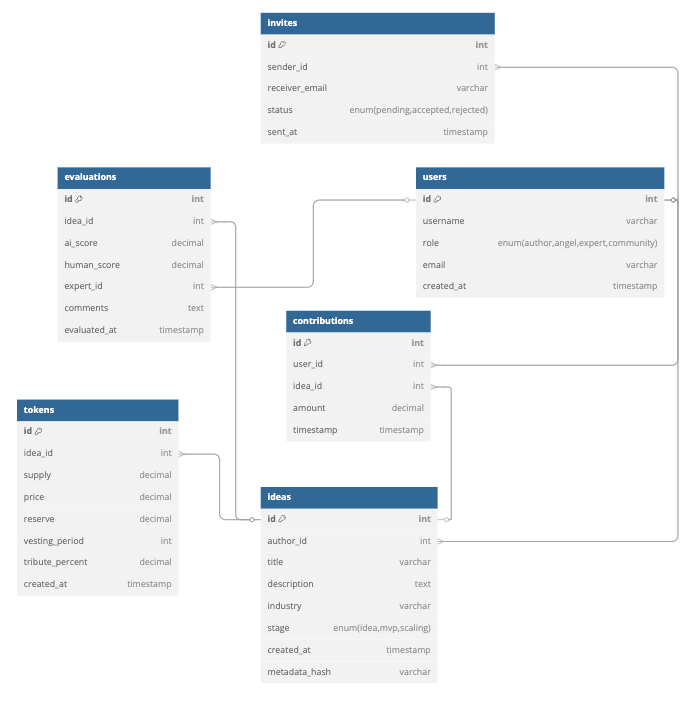
\includegraphics[width=0.5\textwidth]{./assets/database.png}
  \caption{Схема базы данных}
  \label{fig:database}
\end{figure}

Рассмотрим каждую из таблиц базы данных подробнее.

\mysubsection{Таблица Users}
Хранит информацию о зарегистрированных участниках платформы. Пользователи могут иметь одну из ролей: автор идеи, ангел-инвестор, эксперт или участник сообщества.
\begin{itemize}
  \item \texttt{id} --- уникальный идентификатор пользователя
  \item \texttt{username} --- имя пользователя
  \item \texttt{role} --- роль: author, angel, expert, community
  \item \texttt{email} --- адрес электронной почты
  \item \texttt{created\_at} --- дата регистрации
\end{itemize}

\mysubsection{Таблица Ideas}
Таблица идей служит для безопасного хранения зашифрованных идей стартапов на устройствах пользователей до момента их токенизации на блокчейне. Она включает уникальные идентификаторы идей, ссылки на авторов из таблицы пользователей, названия и подробные описания идей (зашифрованные для защиты интеллектуальной собственности), а также информацию об отрасли, стадии развития (идея, MVP или масштабирование), дате создания и хеше метаданных, который используется для последующей верификации на блокчейне.
\begin{itemize}
  \item \texttt{id} --- уникальный идентификатор идеи
  \item \texttt{author\_id} --- внешний ключ на пользователя-автора
  \item \texttt{title} --- название идеи
  \item \texttt{description} --- описание идеи
  \item \texttt{industry} --- отрасль
  \item \texttt{stage} --- стадия развития: idea, mvp, scaling
  \item \texttt{created\_at} --- дата создания
  \item \texttt{metadata\_hash} --- хэш метаданных (например, IPFS)
\end{itemize}

\mysubsection{Таблица Evaluations}
Таблица оценок фиксирует результаты анализа идей, проводимого искусственным интеллектом и людьми, что обеспечивает слепую и объективную оценку для инвестиционных решений.
\begin{itemize}
  \item \texttt{id} --- идентификатор оценки
  \item \texttt{idea\_id} --- ссылка на оцениваемую идею
  \item \texttt{ai\_score} --- оценка ИИ
  \item \texttt{human\_score} --- оценка от сообщества
  \item \texttt{expert\_id} --- эксперт, проводивший оценку
  \item \texttt{comments} --- комментарии к оценке
  \item \texttt{evaluated\_at} --- дата оценки
\end{itemize}

\mysubsection{Таблица Contributions}
Таблица вкладов регистрирует локальные финансовые вложения пользователей в идеи до их токенизации на блокчейне. Эта таблица связывает пользователей и идеи, обеспечивая отслеживание финансовой поддержки.
\begin{itemize}
  \item \texttt{id} --- уникальный идентификатор транзакции
  \item \texttt{user\_id} --- инвестор
  \item \texttt{idea\_id} --- финансируемая идея
  \item \texttt{amount} --- сумма вклада
  \item \texttt{timestamp} --- время вложения
\end{itemize}

\mysubsection{Таблица Tokens}
Таблица токенов управляет локальными данными о токенах, которые будут токенизированы на блокчейне после инвестиций. Таблица связана с таблицей идей, поддерживая механизм распределения ресурсов.
\begin{itemize}
  \item \texttt{id} --- уникальный идентификатор токена
  \item \texttt{idea\_id} --- связанная идея
  \item \texttt{supply} --- объем эмиссии
  \item \texttt{price} --- цена токена
  \item \texttt{reserve} --- резервный пул
  \item \texttt{vesting\_period} --- период вестинга (в днях)
  \item \texttt{tribute\_percent} --- трибьют в процентах
  \item \texttt{created\_at} --- дата выпуска токена
\end{itemize}

\mysubsection{Таблица Transactions}
Таблица транзакций фиксирует все транзакции в системе.
\begin{itemize}
  \item \texttt{id} --- уникальный идентификатор транзакции
  \item \texttt{sender\_id} --- отправитель транзакции
  \item \texttt{receiver\_email} --- email приглашённого
  \item \texttt{status} --- статус: pending, accepted, rejected
  \item \texttt{sent\_at} --- дата отправки
\end{itemize}

Такая структура базы данных обеспечивает эффективную работу распределённых децентрализованных приложений, взаимодействующих с внешними источниками данных и блокчейн-сетями. Она поддерживает атомарность транзакций, обеспечивает целостность данных и позволяет масштабировать систему при увеличении нагрузки. Особое внимание уделено оптимизации запросов и индексации ключевых полей для быстрого доступа к данным. Структура также учитывает необходимость синхронизации с блокчейн-сетью и обеспечивает хранение метаданных для каждой операции.

% ## 4.4
\mysection{Разработка серверной части}

В качестве серверного фреймворка в разработанном приложении использовался Fastify --- современный, асинхронный и высокопроизводительный веб-фреймворк для Node.js. Он предоставляет поддержку JSON Schema для валидации входящих и исходящих данных, а также встроенные хуки жизненного цикла, плагины, систему маршрутизации и встроенные механизмы сериализации. Благодаря минималистичной архитектуре Fastify, удалось значительно ускорить запуск API и уменьшить накладные расходы при масштабировании.
Для обработки данных и взаимодействия с базой данных применялась PostgreSQL

С целью улучшения взаимодействия пользователей и администраторов платформы был разработан Telegram-бот, использующий асинхронную библиотеку Asyncio и фреймворк python-telegram-bot. Данный бот выполняет функцию модерации и валидации идей, предоставляя администраторам удобный интерфейс для проверки и одобрения проектов. При поступлении новой идеи администратор получает уведомление в Telegram, содержащее всю необходимую информацию для принятия решения. После валидации администратором система автоматически отправляет уведомления пользователям о статусе проверки их идей, тем самым обеспечивая оперативную обратную связь.

\begin{figure}[H]
  \centering
  
\includegraphics[width=0.5\textwidth]{./assets/telegram-bot.png}
  \caption{Сообщения валидации для администрата и пользователя}
  \label{fig:telegram-bot}
\end{figure}

Мониторинг состояния серверной инфраструктуры осуществляется с помощью логирования запускамеого с переодичностью в 5 минут с помощью утилиты cron. Это позволяет оперативно реагировать на возникающие инцинденты. Кроме того, Telegram-бот используется для отправки администратору сообщений в случае критических событий и ошибок состояний системы в реальном времени. Сбор и анализ логов также производятся через интеграцию с отдельным Telegram-ботом, который автоматически отправляет уведомления о состоянии и событиях системы администраторам платформы. Это позволяет быстро реагировать на потенциальные проблемы и оперативно устранять их. Подобная схема мониторинга и логирования гарантирует базовый уровень доступности и отказоустойчивости, а также значительно упрощает процесс мониторинга состояния платформы.

% ## 4.5
\mysection{Разработка прототипа приложения}

Интерфейс прототипа разработан с учетом принципов интуитивности и простоты взаимодействия, обеспечивая при этом доступ ко всему функционалу системы.
Общая схема взаимодействия компонентов прототипа представлена на рисунке \ref{fig:app-prototype}, где проиллюстрированы основные процессы и связи между элементами системы.

\begin{figure}[H]
  \centering
  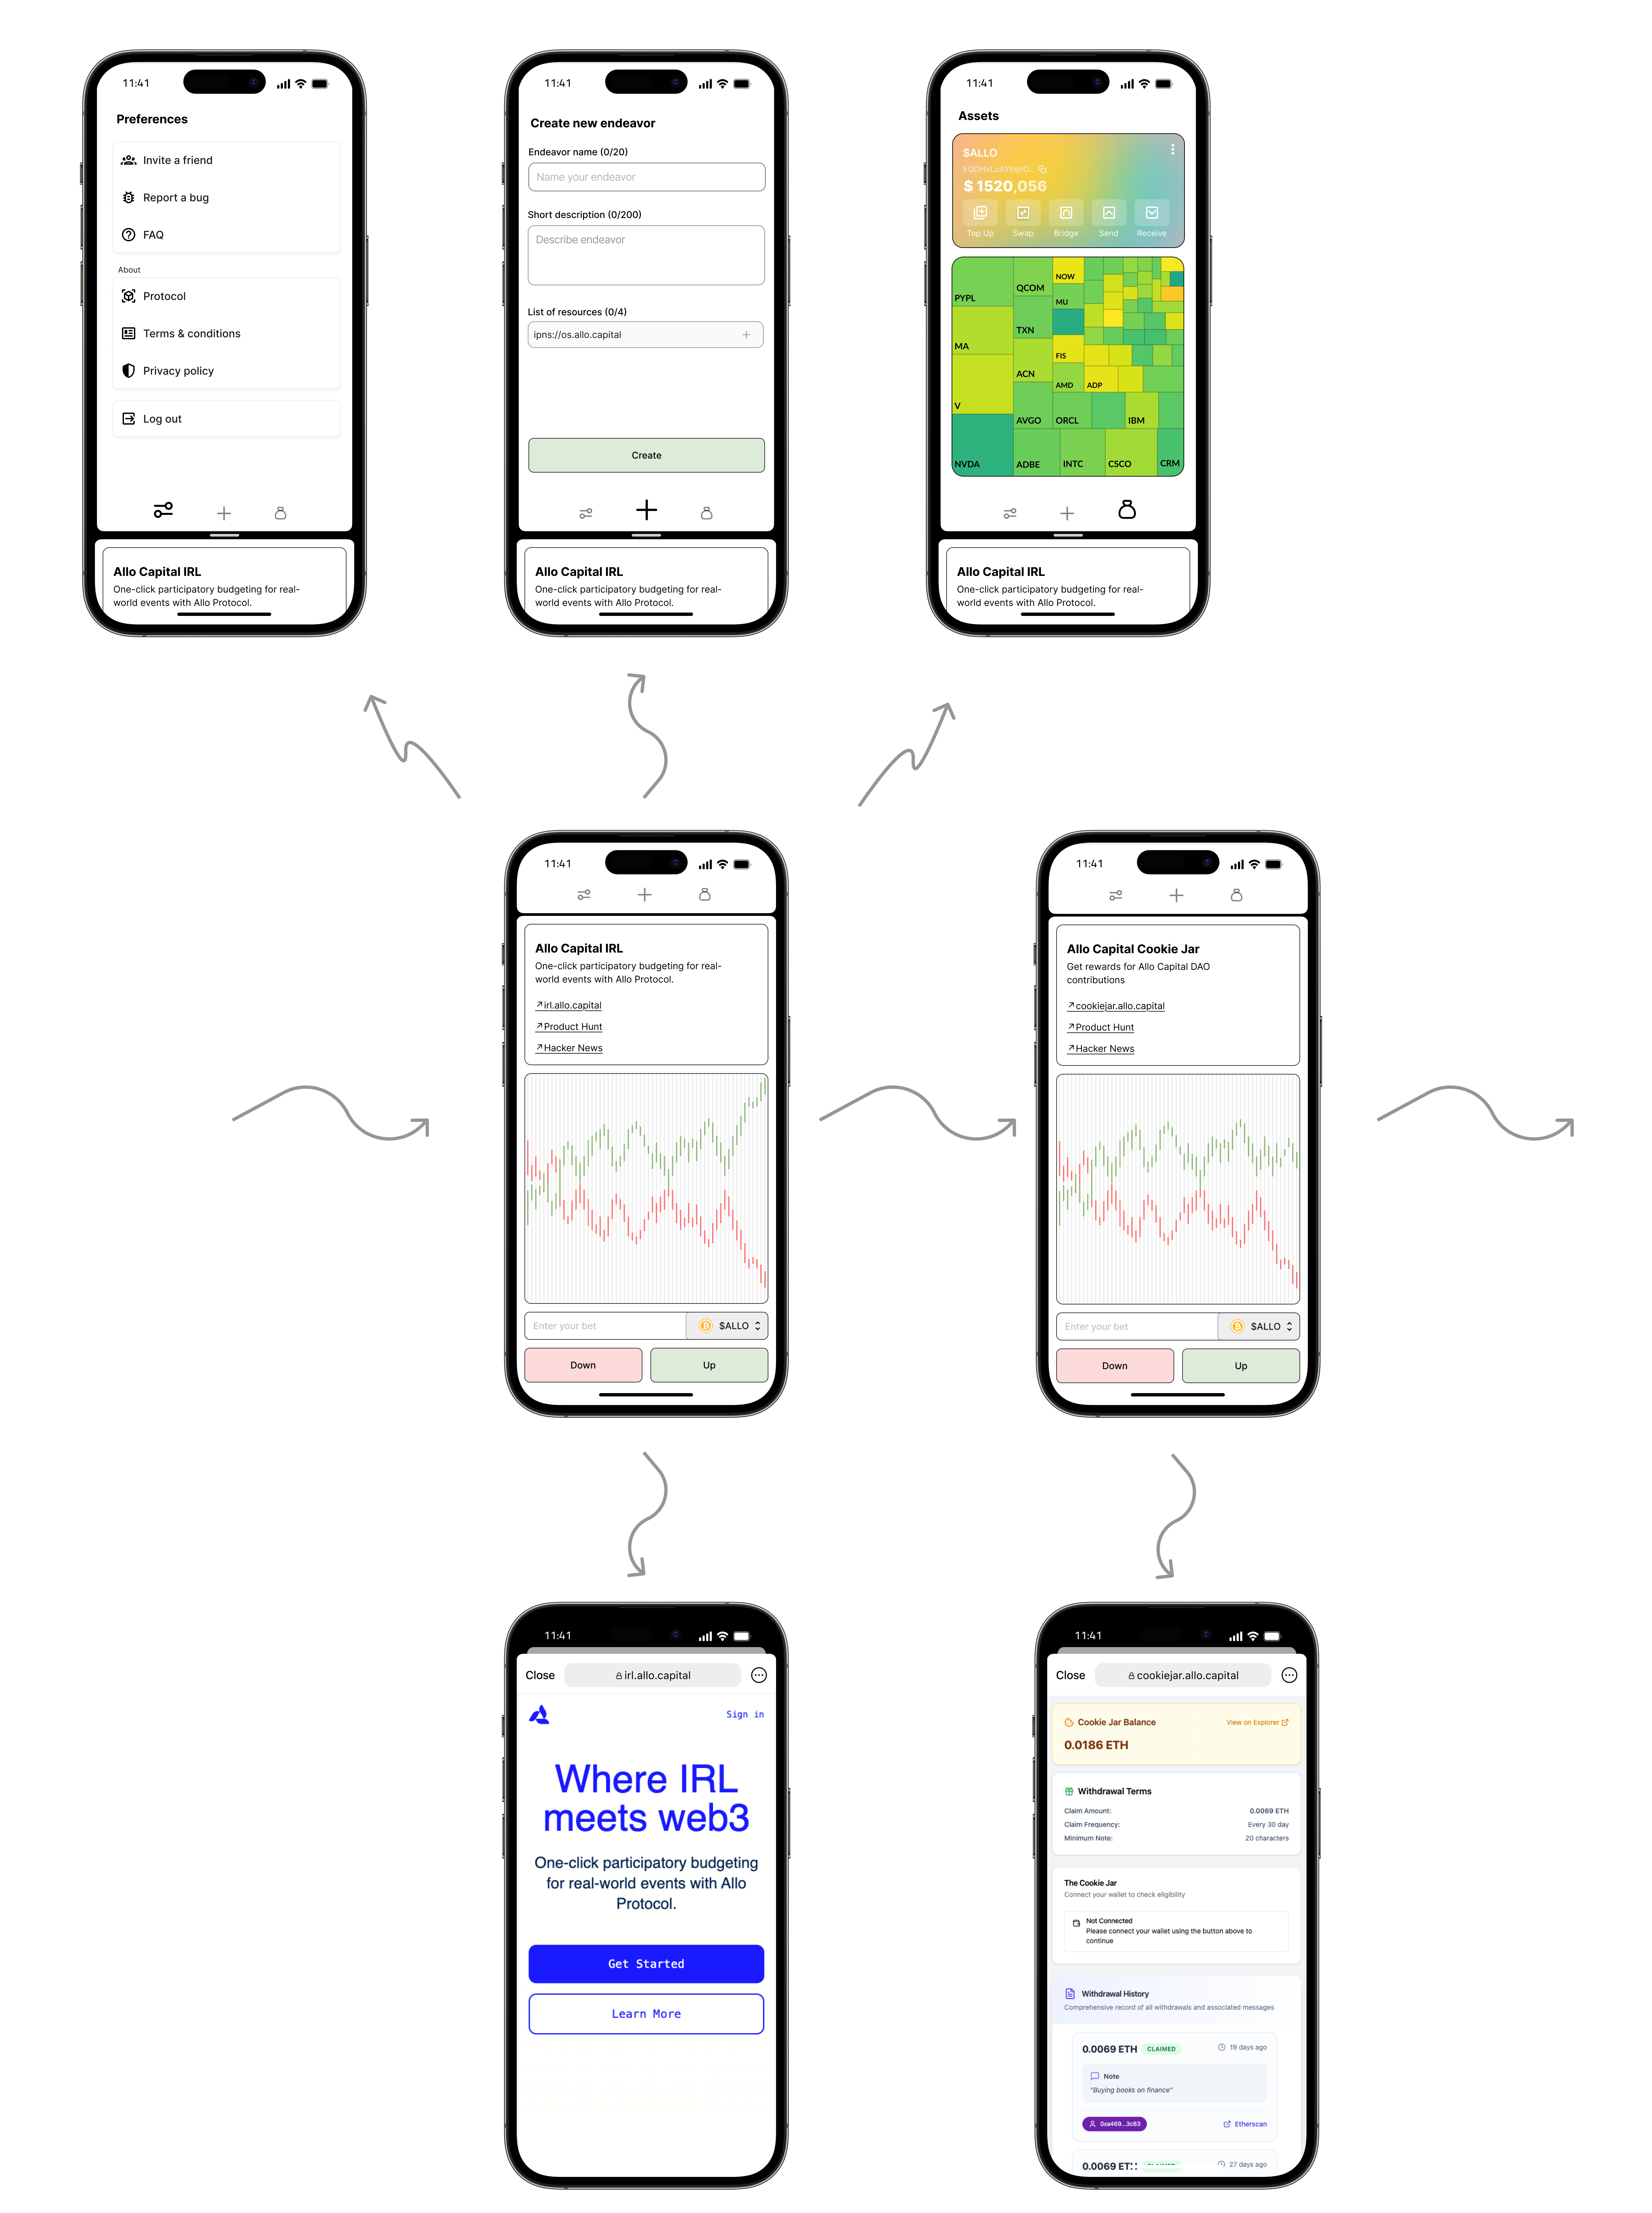
\includegraphics[width=0.5\textwidth]{./assets/app-prototype.png}
  \caption{Схема основных процессов и взаимодействий в прототипе платформы}
  \label{fig:app-prototype}
\end{figure}


Прототип компонента навигации показан на рисунке \ref{fig:app-navigation}.

\begin{figure}[H]
  \centering
  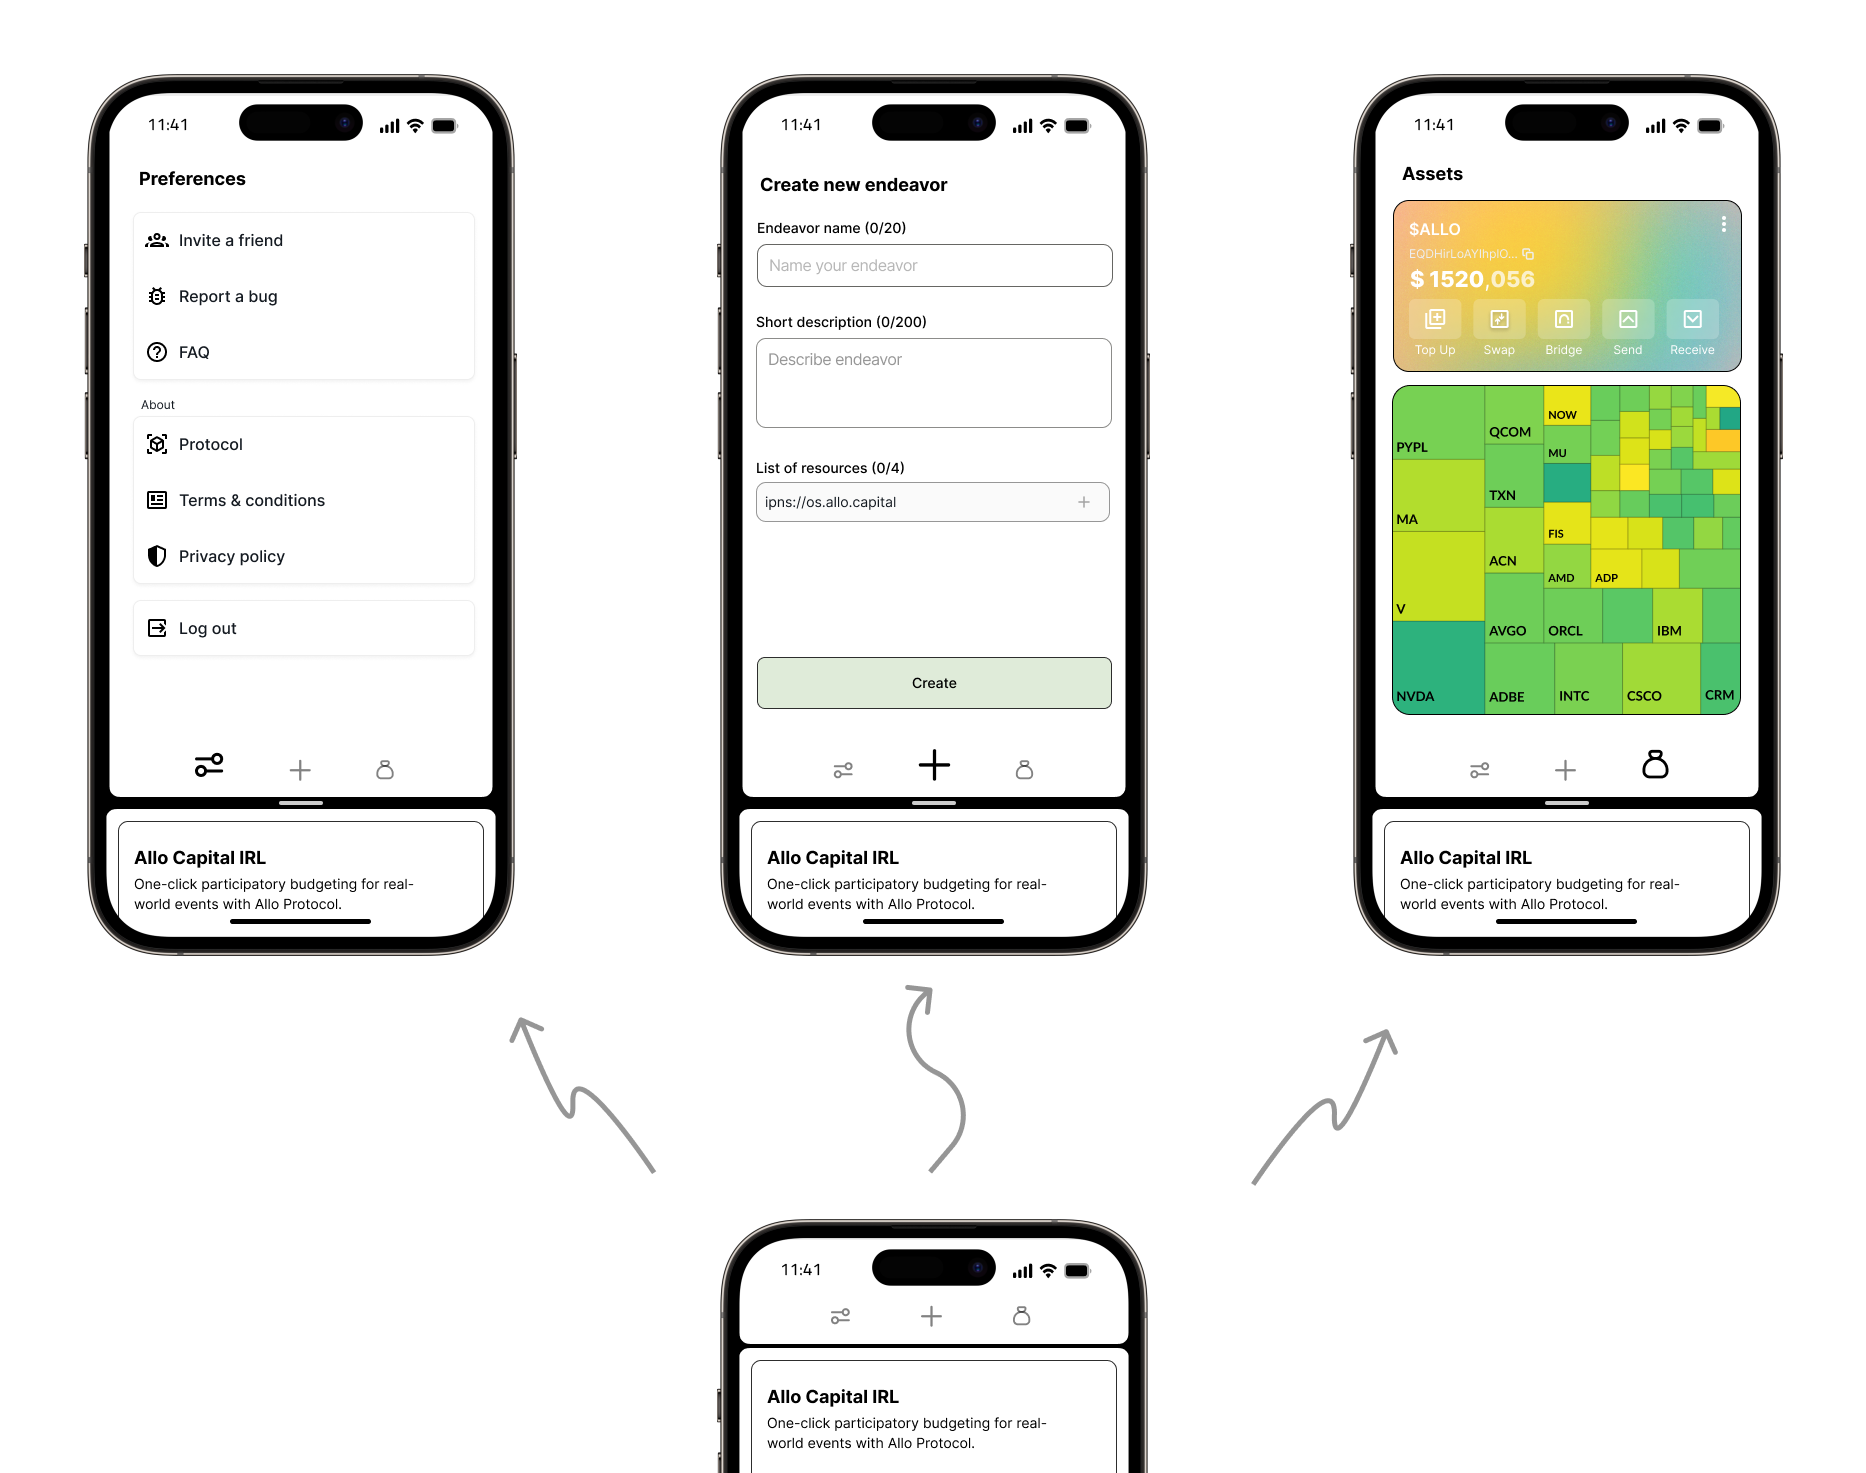
\includegraphics[width=0.5\textwidth]{./assets/app-navigation.png}
  \caption{Экран навигации между модулями приложения}
  \label{fig:app-navigation}
\end{figure}

% ### 4.5.1
\mysubsection{Разработка дизайн системы}

Дизйн был выполнен с помощью Figma.

Особое внимание было уделено визуальному оформлению приложения с учетом портрета целевой аудитории. Визульное оформление, выбор цветовой палитры, шрифтов и икорон были основыны на создании положительных эмоций, подчеркивая новизну и смелость.
Логотип представлен на рисунке \ref{fig:app-logo}.

\begin{figure}[H]
  \centering
  
\includegraphics[width=0.2\textwidth]{./assets/app-logo.png}
  \caption{Логотип приложения}
  \label{fig:app-logo}
\end{figure}

Дизайн-система приложения включает в себя набор переиспользуемых компонентов, обеспечивающих единообразие интерфейса и упрощающих разработку. Все компоненты содержат прозрачный фон с эффектом размытия. Компоненты реализованы с учетом адаптивности под различные размеры экранов и ориентации устройства. Компоненты представлены на рисунке \ref{fig:components}.

\begin{figure}[H]
  \centering
  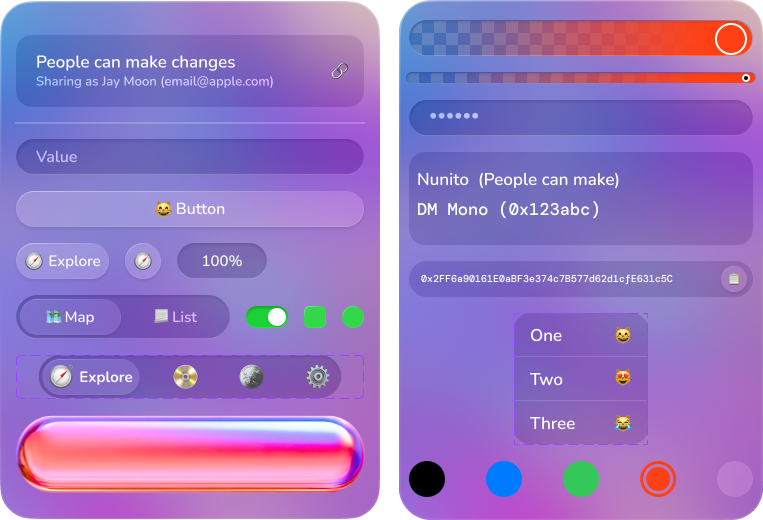
\includegraphics[width=0.5\textwidth]{./assets/components.png}
  \caption{Прототип компонентов системы}
  \label{fig:components}
\end{figure}

% ### 4.5.2
\mysubsection{Главный экран приложения}

Основной сценарий использования приложения. На нём отображается ключевая информация и основные действия, доступные сразу после запуска. В верхней части располагается заголовок приложения или логотип, а также кнопки навигации (например, кнопка меню для перехода к экрану навигации между модулями).

Центральное пространство главного экрана отведено под список текущих инициатив или проектов. Каждая инициатива представлена в виде карточки или строки: содержит название инициативы и её краткое описание. В прототипе на карточке отображается название проекта и одна строка с описанием его цели или сути. Кроме того, под описанием располагаются иконки или ссылки на внешние ресурсы, связанные с этой инициативой (например, иконки Product Hunt или Hacker News, если инициатива упоминается на этих платформах).

Раскрытие лиц увеличивает вероятность успеха инициативы на 3\% \cite{farrel2024leveraging}

Основное назначение главного экрана – предоставить пользователю обзор актуальных инициатив и быстрый доступ к дальнейшим действиям. Пользователь может прокручивать список для просмотра всех доступных инициатив. Нажатие на карточку инициативы приводит к переходу на экран браузера, где раскрываются подробности выбранного проекта в виде встроенной веб-страницы.

С главного экрана также доступен переход к созданию новой инициативы – это реализовано через отдельную кнопку (значок «+» на панели) или через меню навигации. Пример отображения главного экрана приведён на рисунке \ref{fig:app-main-flow}.

\begin{figure}[H]
  \centering
  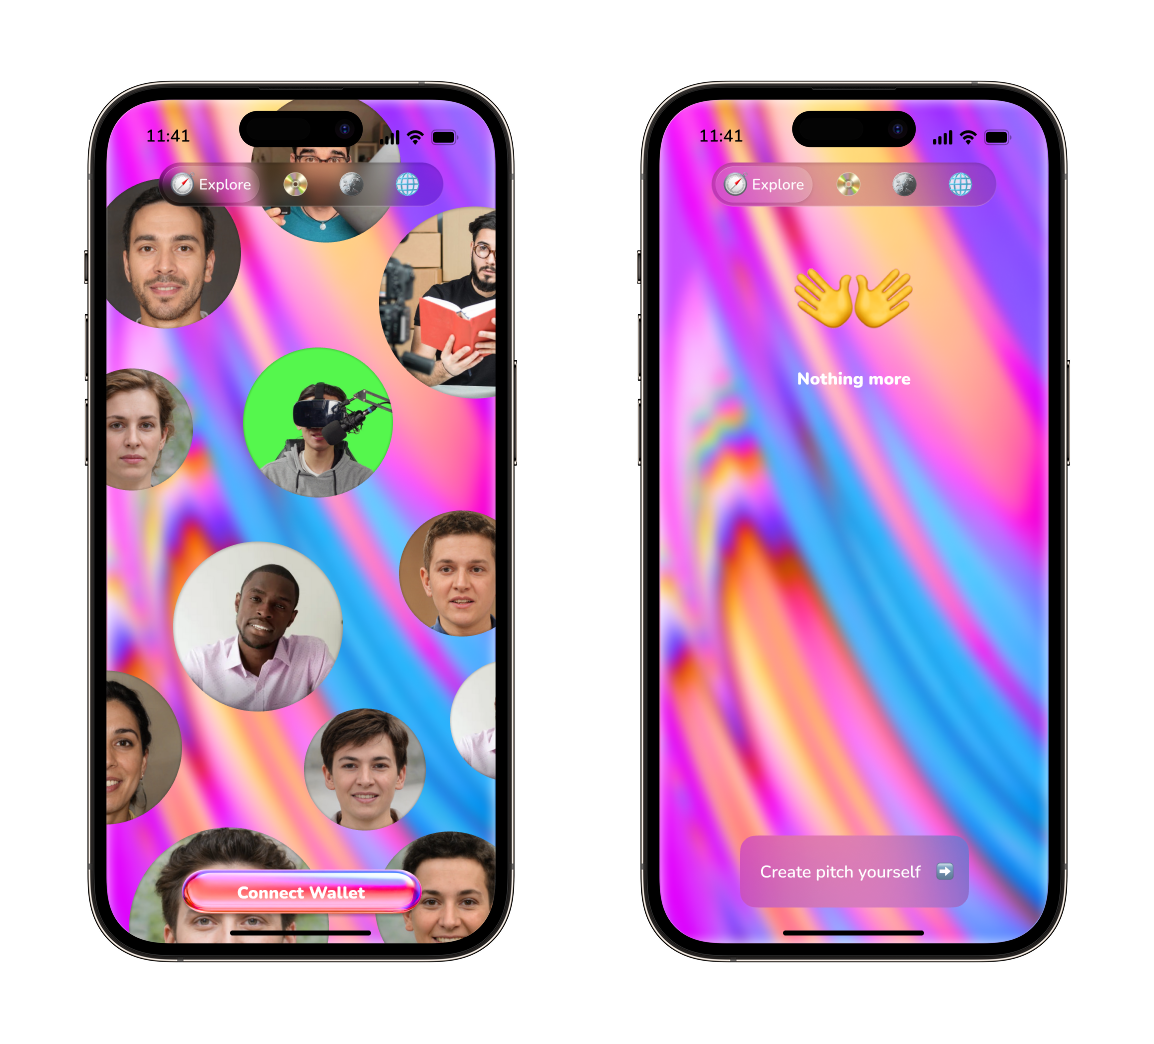
\includegraphics[width=0.5\textwidth]{./assets/app-main-flow.png}
  \caption{Главный экран приложения со списком инициатив}
  \label{fig:app-main-flow}
\end{figure}

% #### 4.5.2
\mysubsection{Экран управления активами и финансами}

Экран управления активами предоставляет пользователю сведения о его финансовых ресурсах в приложении. Здесь отображаются все доступные активы (например, внутренние токены или валюты, связанные с платформой).

Интерфейс организован в виде списка кошельков или счетов: каждая строка представляет отдельный актив с указанием его названия или тикера, идентификатора (например, часть адреса кошелька) и текущего баланса. В прототипе присутствует актив с кодом --- рядом с ним показан уникальный идентификатор (адрес счёта или номер кошелька) и баланс, выраженный числом (например, 1,520,056).

Для каждого актива предусмотрены отдельные управляющие элементы: кнопки действий для управления средствами, такие как «Top Up» (пополнить), «Swap» (обменять), «Bridge» (перевести между сетями), «Send» (отправить) и «Receive» (получить). Ниже основного актива также отображается тепловая карта инвестиций по различным проектам, что позволяет пользователю визуально оценить распределение своих активов.

\begin{figure}[H]
  \centering
  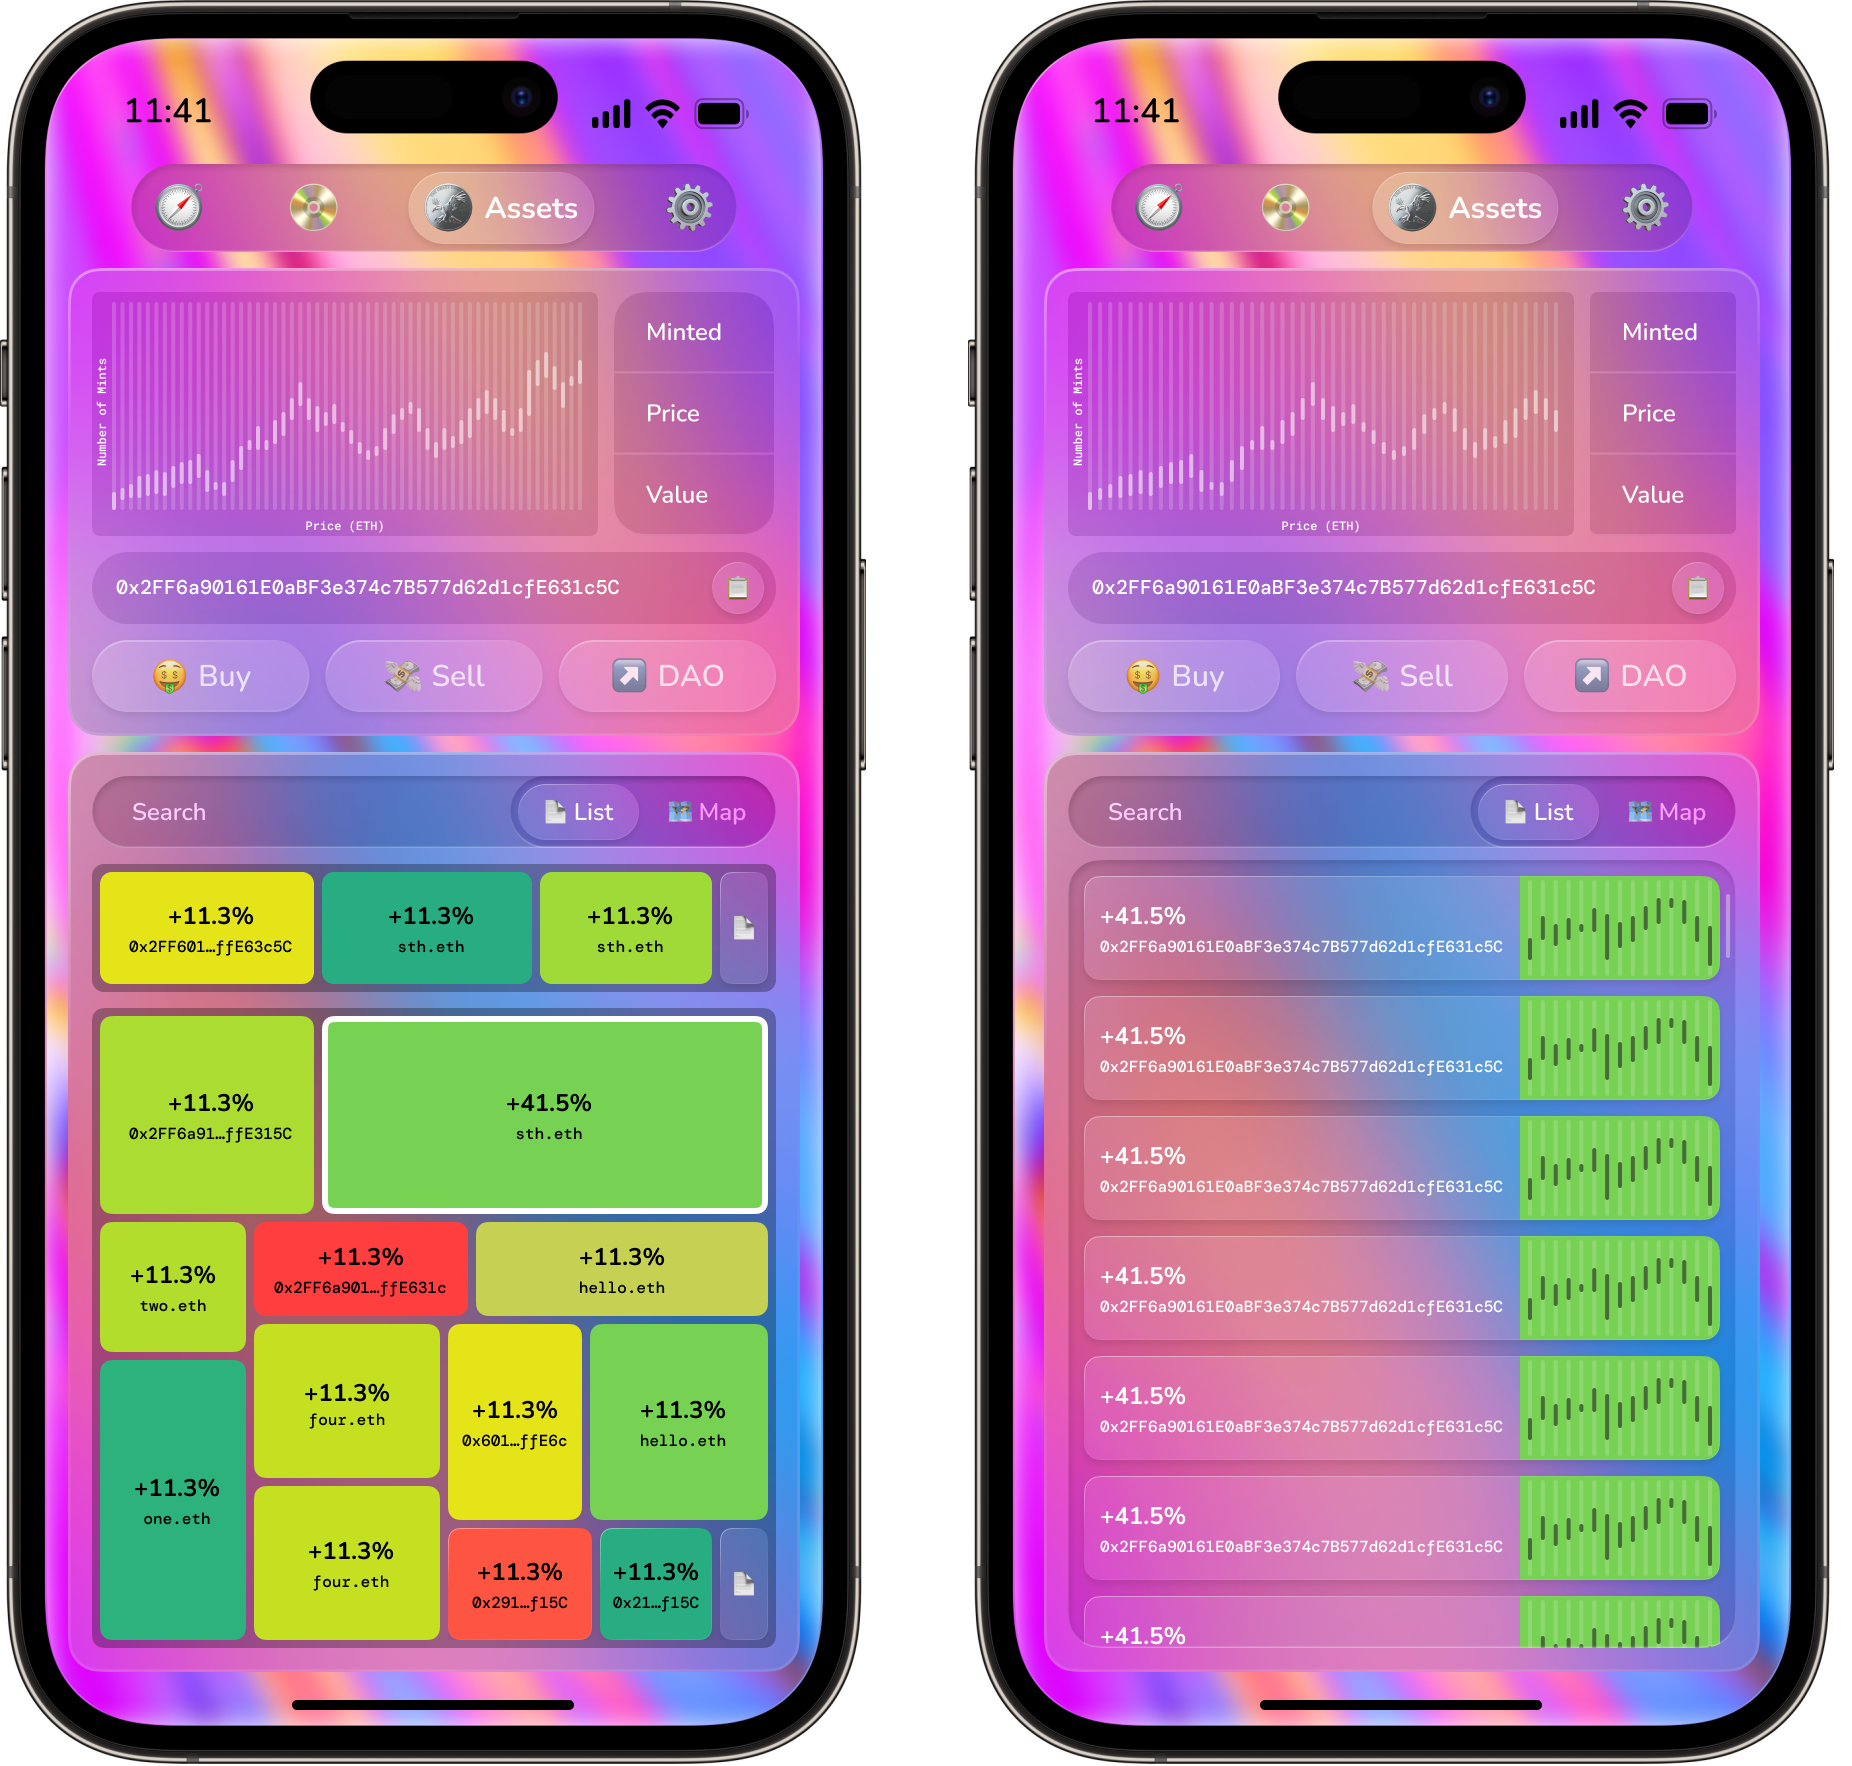
\includegraphics[width=0.5\textwidth]{./assets/app-assets.png}
  \caption{Пример экрана управления активами и финансами}
  \label{fig:app-assets}
\end{figure}

Типичный сценарий использования: пользователь переходит в этот раздел, чтобы проверить достаточен ли у него баланс для участия в той или иной инициативе, либо чтобы просмотреть результаты предыдущих взаимодействий.

% #### 4.5.3
\mysubsection{Экран создания новой инициативы}

Экран создания нового видео позволяет пользователю добавить свой собственный проект или предложение в систему. Это форма ввода данных, где последовательно представлены поля, необходимые для описания инициативы.

На экране отображается заголовок формы «Create» (Создать новую инициативу) для ясности. Затем присутствует блок для добавления связанных ресурсов или ссылок. В прототипе есть раздел, куда пользователь может добавить ссылку на обсуждение инициативы (рисунок \ref{fig:app-create}).

\begin{figure}[H]
  \centering
  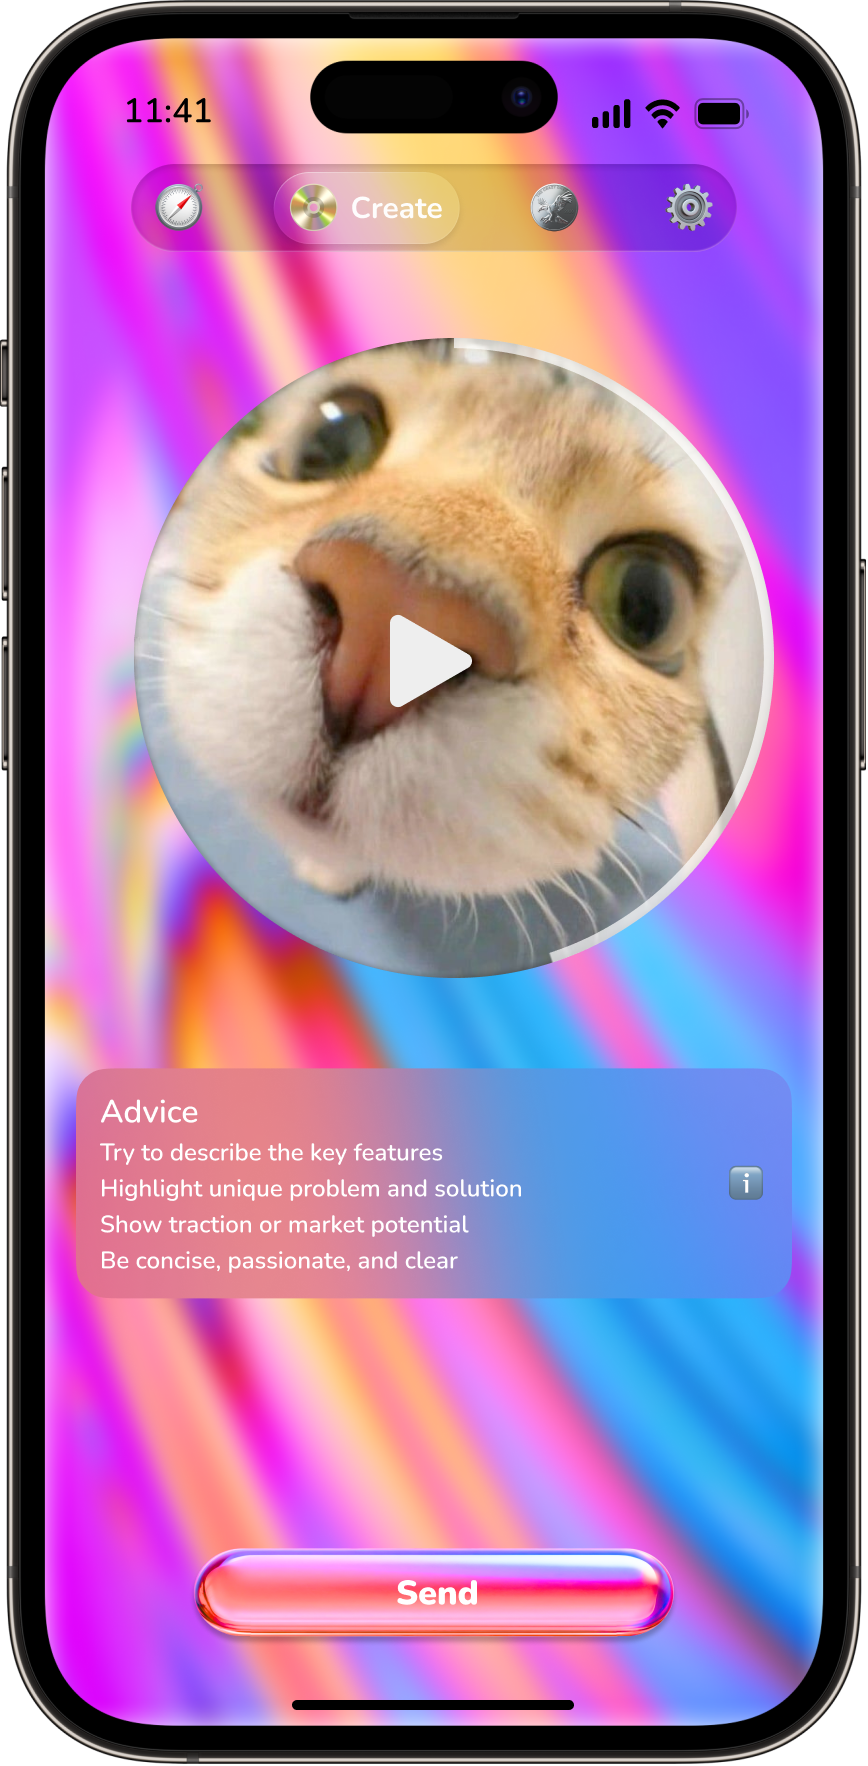
\includegraphics[width=0.5\textwidth]{./assets/app-create.png}
  \caption{Пример экрана создания новой инициативы}
  \label{fig:app-create}
\end{figure}

После заполнения необходимых полей активируется кнопка «Send» (Отправить), расположенная в нижней части формы. Нажатие этой кнопки отправляет инициативу администратору на валидацию. Позже пользователь получит сообщение в Telegram с результатом валидации.

% #### 4.5.4
\mysubsection{Экран настроек пользователя}

Экран настроек пользователя содержит опции для персонализации и обслуживания аккаунта. Этот раздел включает различные пункты, сгруппированные по тематике. В прототипе часть этих пунктов уже видна в меню навигации: например, «Preferences» (общие настройки), «Invite a friend» (приглашение новых пользователей), «Report a bug» (сообщение об ошибке разработчикам), «FAQ» (ответы на частые вопросы), и другие.

На экране настроек эти пункты представлены списком кнопок или ссылок. Нажатие на каждый из них приводит к соответствующему действию или открывает дополнительную информацию. Например, выбор «Preferences» открывает подэкран с настройками (переключателями и опциями, такими как уведомления, язык интерфейса). Выбор «Invite a friend» вызывает окно шаринга или копирует реферальную ссылку.

Экран настроек также отвечает за связь пользователя с системой в целом. Здесь расположен пункт «Log out» (Выход), с помощью которого пользователь может выйти из своего аккаунта или отключить текущую сессию.

С точки зрения сценариев, пользователь обращается к экрану настроек по необходимости: изменить что-то в профиле, узнать информацию о приложении, связаться с поддержкой или выйти из системы. Пример экрана настроек можно увидеть на рисунке \ref{fig:app-settings}.

\begin{figure}[H]
  \centering
  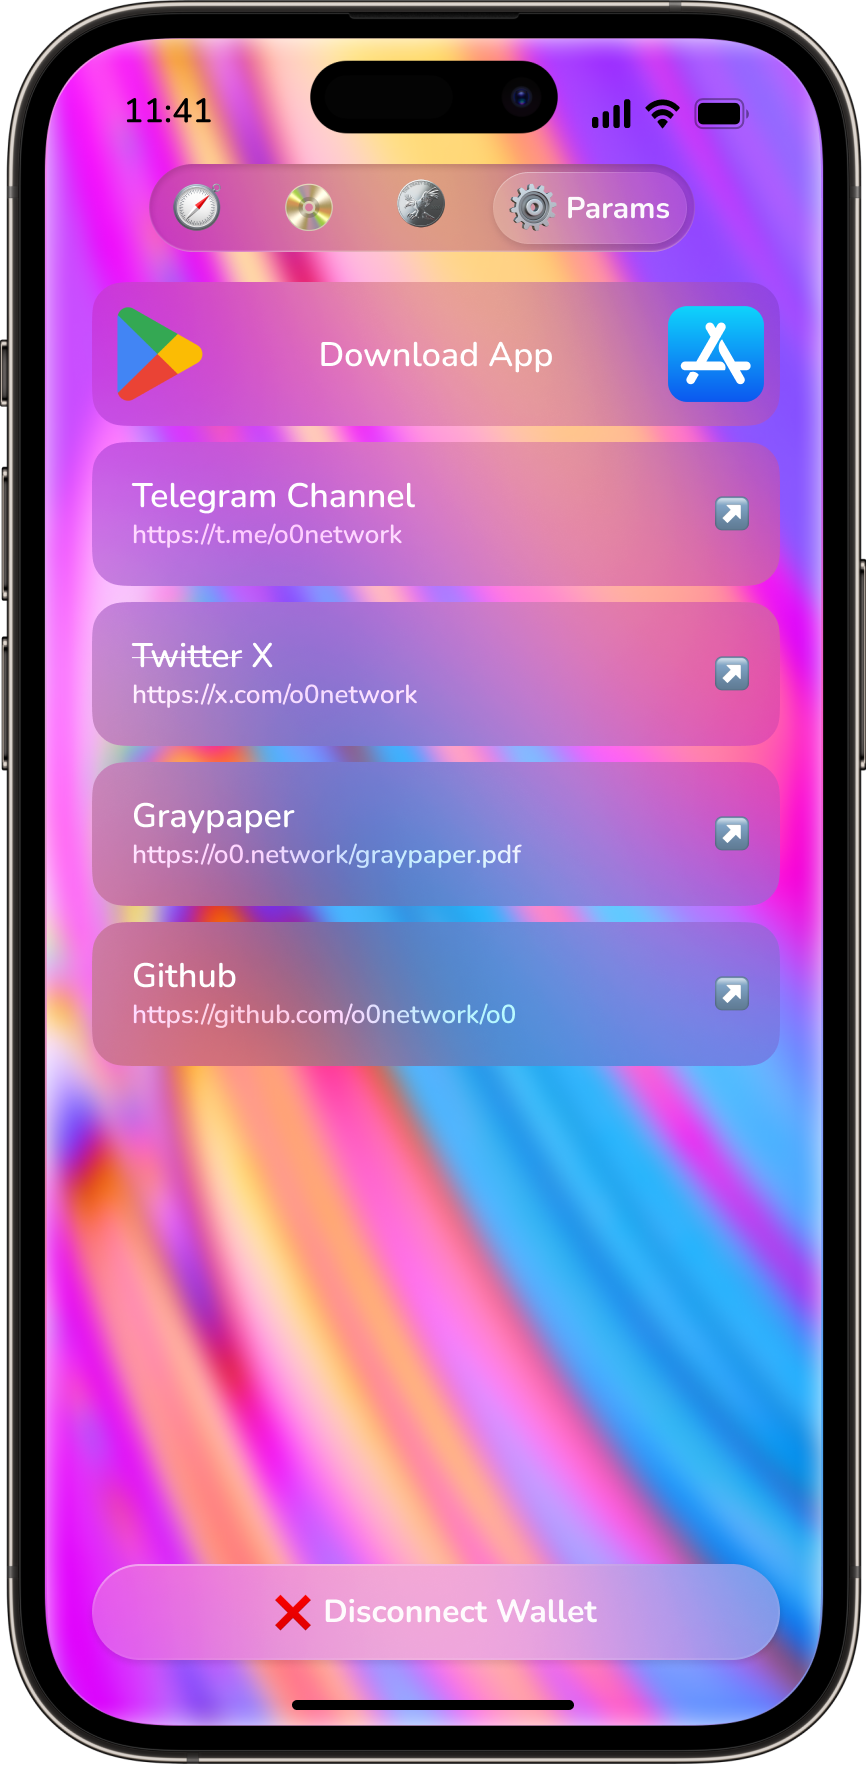
\includegraphics[width=0.5\textwidth]{./assets/app-settings.png}
  \caption{Пример экрана настроек пользователя}
  \label{fig:app-settings}
\end{figure}

% ### 4.5.6
\mysubsection{Экран браузера}

Экран браузера предназначен для отображения детальной информации об инициативе посредством встроенного веб-браузера. Этот экран открывается, когда пользователь выбирает инициативу на главном экране или нажимает на связанный с ней внешний ресурс.

В верхней части экрана браузера присутствует панель навигации: она содержит кнопку «Назад» для возвращения к предыдущему экрану (например, обратно к главному списку) и отображает адрес или название ресурса, который просматривается. Основное пространство занимает содержимое веб-страницы, связанной с выбранной инициативой.

Во время просмотра встроенной страницы пользователь может взаимодействовать с ней так же, как в обычном браузере: прокручивать контент, нажимать на ссылки или кнопки. При этом, благодаря встроенному браузеру, нет необходимости покидать приложение. Пример экрана браузера представлен на рисунке \ref{fig:app-browser}.

\begin{figure}[H]
  \centering
  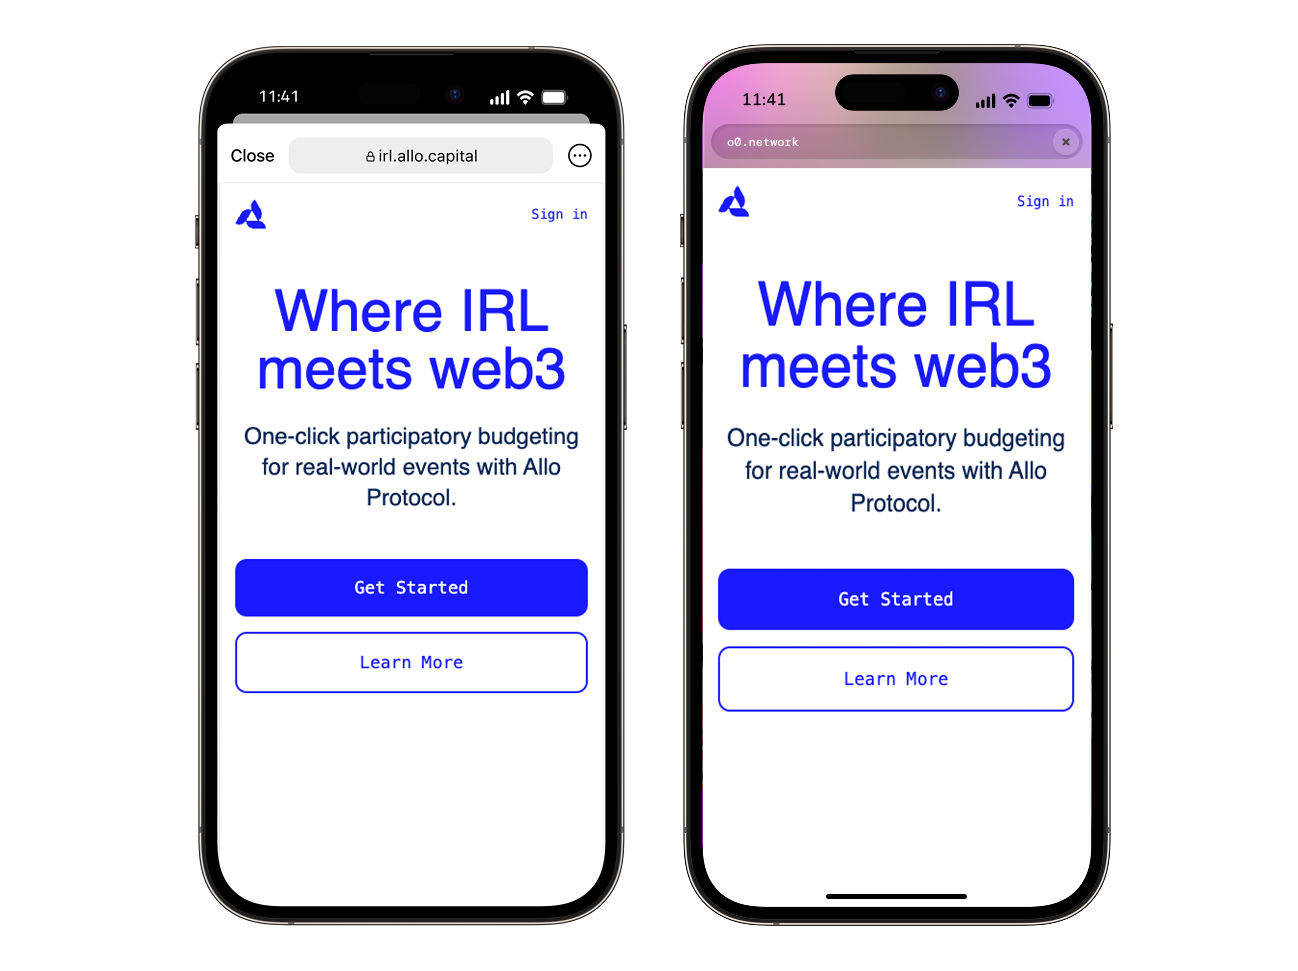
\includegraphics[width=0.5\textwidth]{./assets/app-browser.png}
  \caption{Пример экрана браузера с детальной информацией о проекте}
  \label{fig:app-browser}
\end{figure}

Все представленные экраны в совокупности формируют комплексное пользовательское взаимодействие с платформой, обеспечивая доступ ко всему функционалу системы через интуитивно понятный мобильный интерфейс.

% ## 4.6
\mysection{Разработка клиентской части}

Клиентская часть представляет собой мобильное приложение, которое работает на различных платформах, включая мобильные операционные системы, веб и мессенджеры. Приложение использует современные библиотеки для управления данными и работы с криптовалютами. Архитектура построена по модульному принципу, что обеспечивает удобство поддержки и масштабирования кода.

% ### 4.6.1
\mysubsection{React Native}

Мобильное приложение реализовано с использованием React Native и фреймворка Expo. Это позволило обеспечить мультиплатформенность и запуск приложения на iOS, Android, Web и Telegram Mini Apps без необходимости поддержки нескольких кодовых баз. React Native позволил повторно использовать UI-компоненты и бизнес-логику между платформами.

Архитектура приложения реализована по принципам Feature-Sliced Design (FSD), что обеспечивает модульность, предсказуемость структуры и лёгкость масштабирования. В соответствии с FSD, код организован в слои: app, pages, widgets, features, entities, shared. Каждый слой содержит тематические слайсы, разделённые на сегменты (ui, model, api, lib).

Для синхронизации клиентского состояния с сервером используется библиотека TanStack Query (ранее React Query). Она обеспечивает декларативное взаимодействие с API, кэширование запросов, автоматическое обновление данных и обработку ошибок. TanStack Query позволяет унифицировать доступ к данным и упрощает поддержку бизнес-логики, особенно в условиях высокой частоты обновления данных.

Для подключения к криптокошелькам в мобильной версии используется WalletConnect. Это открытый протокол, позволяющий подключать децентрализованные приложения к мобильным кошелькам с помощью QR-кодов или deep link-ссылок. Реализация WalletConnect обеспечивает механизм авторизации и безопасное взаимодействие с Web3-сервисами, отправку транзакций и подписание сообщений в пользовательском интерфейсе без прямого доступа к приватным ключам.

При реализации интерфейса особое внимание уделялось мобильной адаптивности и совместимости с Telegram Mini Apps. Использовались компоненты react-native-web и react-native-router, а для WebView-интеграции применялись средства Telegram WebApp SDK.

% ### 4.6.2
\mysubsection{Telegram Mini Apps}

Telegram Mini Apps это внутренняя веб-платформа Telegram, позволяющая запускать полнофункциональные веб-приложения (HTML/JS) внутри чата. Mini Apps используются для показа отдельного интерфейса (например, каталог инициатив или вкладка инвестирования) без необходимости переключаться в внешнее приложение. Это обеспечивает более «нативный» пользовательский опыт: Mini Apps «простой, гибкий, выглядит как родное веб-приложение, повышает удобство взаимодействия». С помощью Mini Apps пользователи могут, например, просматривать описание инициатив и совершать действия (голосовать, инвестировать) прямо из чата Telegram, получая полноценный UI, интегрированный в мессенджер.

% ### 4.6.3
\mysubsection{Главная страница}

Дополнительно был разработан лендинг веб-сайт, который позволяет пользователям ознакомиться с платформой и её возможностями. Она была разработана с использованием html, css и javascript (Рисунок \ref{fig:landing-page}).

\begin{figure}[H]
  \centering
  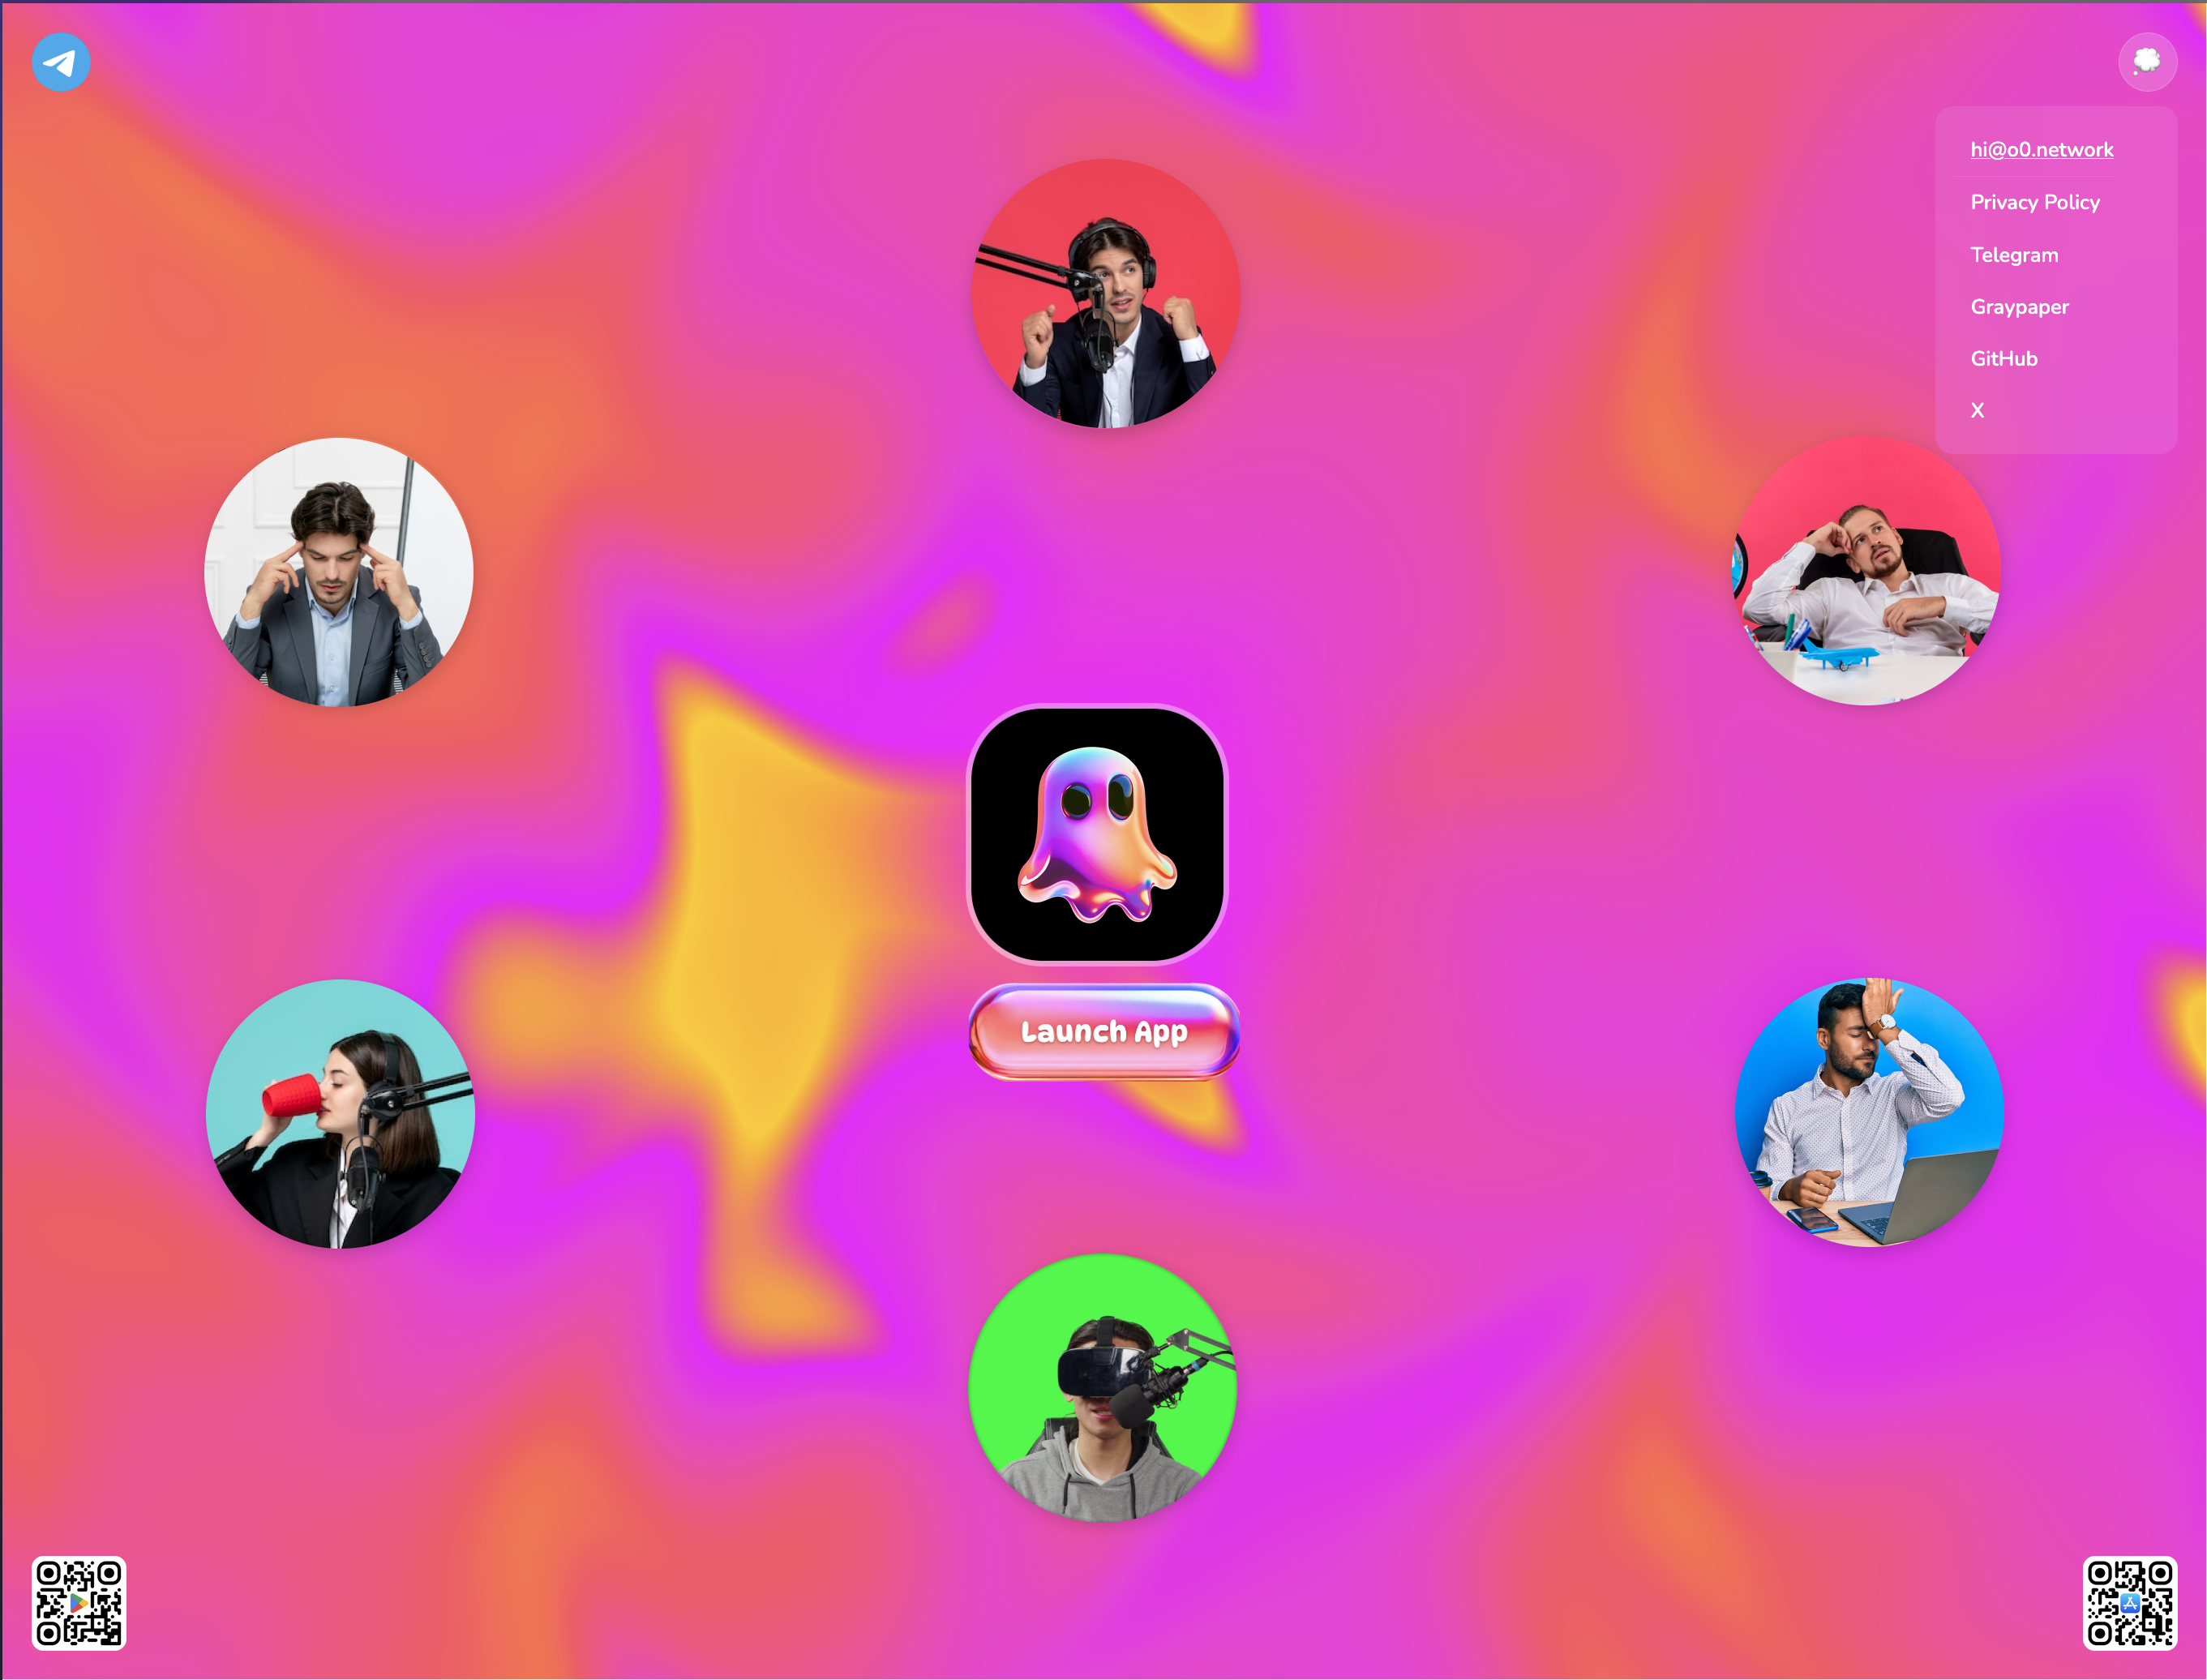
\includegraphics[width=0.8\textwidth]{./assets/landing-page.png}
  \caption{Лендинговая страница}
  \label{fig:landing-page}
\end{figure}

На странице размещены кнопка для открытия телеграм бота, меню с дополнительными ссылкми, QR-коды для загрузки мобильного приложения на ios и android. Центр страницы занимает логотип приложения CTA кнопка --- «Launch App». Вокруг логотипа размещены круглые видеоролики с объеснением базовых принципов механизма распределения ресурсов в приложении. Ролики создают ощущение сообщества.  В левом верхнем углу находится иконка Telegram, в правом верхнем углу — выдвигаемое меню с контактным email и навигационными ссылками (Privacy Policy, Telegram, Graypaper, GitHub). В нижних углах экрана расположены QR-коды для быстрого перехода на мобильные приложения. Такой дизайн подчёркивает современный и эмоционально вовлекающий стиль лендинга.

% ## 4.7
\mysection{Вывод по четвертой главе}

В данной главе была описана реализация децентрализованного инвестиционного приложения в соответствии с архитектурной моделью, рассмотренной ранее. Мы рассмотрели бизнес-процессы (создание инициатив, коллективная оценка, распределение инвестиций и управление активами) и проиллюстрировали, как они поддерживаются выбранными технологиями. Архитектура системы комбинирует фронтенд на React/Expo с надёжной серверной частью на Python и реляционной БД PostgreSQL, дополняя её распределённым хранением данных через IPFS. Непрерывная интеграция и развертывание осуществляются с помощью GitHub Actions, что позволяет оперативно поставлять новые версии приложения. Клиентская часть обеспечивает удобные экраны (главный дашборд, создание инициатив, управление активами и др.), а интеграция с Telegram (бот и Mini Apps) открывает дополнительные каналы взаимодействия с пользователями. Таким образом, реализованный прототип приложения сочетает современные инструменты разработки с концепциями блокчейн-проектов и коллективного инвестирования, создавая основу для дальнейшего развития и внедрения в реальную экосистему.

% ###################################################
% ## Глава 5
% ###################################################

\mychapter{ПЕРСПЕКТИВЫ РАЗВИТИЯ}

В этой главе рассматриваются направления масштабирования и потенциальные области применения описанной системы за рамки инвестиционной платформы. Основное внимание уделено переносу базовой модели, состоящей из взаимодействия агентов, среды и регулирующего механизма, в прикладные сценарии.

\mysection{Масштабирование инвестиционной платформы}

Монетизация системы может происходить за счёт стейкинга пула ликвидности, а управление механизмом в перспективе может быть реализовано посредством community notes. В долгосрочной перспективе возможен выпуск стейблкоинов, обеспеченных пулами ликвидности и привязанных к стабильным активам, что значительно расширит функционал и доступность системы для пользователей и инвесторов.

Дальнейшее развитие платформы инвестирования организовано в виде последовательного поэтапного процесса, каждый этап которого имеет чётко определённые цели, задачи и показатели успеха. На первой фазе создаётся минимально жизнеспособный продукт, направленный на проверку ключевых концепций, привлечение ограниченной группы ранних пользователей, сбор первичной обратной связи и валидацию основных гипотез.

\mysection{Обобщение результатов}

Стоит отметить, что при каждый агент может реализовываться аналогичная структура, образуя рекурсивно вложенную среду: на уровне мета-игры «правила игры» сами настраиваются (через AI-стирающую компоненту), а на нижних уровнях ведётся локальная оптимизация под заданные стимулы.

Аналогичные принципы уже лежат в основе блокчейн-экосистем, где участники, действуя в собственных интересах, стабильно поддерживают целостность и актуальность распределённого реестра создавая консенсус.

AI помогает расширять возможности человека, блокчейн про колобарацию


% ## 5.3
\mysection{Практическое применение}

Базовая структура, разработанная в предыдущих главах — а именно система, состоящая из агентов, среды и регулирующего механизма, — может быть перенесена в другие прикладные сценарии. Эта модель универсальна, так как допускает адаптацию под любые условия, в которых множество участников взаимодействует с окружающей средой, принимая решения и получая обратную связь в виде результатов или вознаграждений.

Ниже приведены примеры альтернативные примеры применения вне контекста инвестиционного распределения ресурсов.

% ## 5.3.1
\mysubsection{ИИ блогер}

В данной модели рассматривается сценарий, в котором языковая модель выступает в роли автономного блогера — информационного агента, взаимодействующего с медиаплатформой и аудиторией как с внешней средой. Основной задачей агента является публикация последовательности постов, содержащих как контентные, так и рекламные элементы, с целью удержания охвата при максимизации ожидаемого дохода. Такая постановка задачи отражает классическую дилемму между долгосрочной лояльностью аудитории и краткосрочной монетизацией (рисунок \ref{fig:ai-blogger-flow}).

\begin{figure}[H]
  \centering
  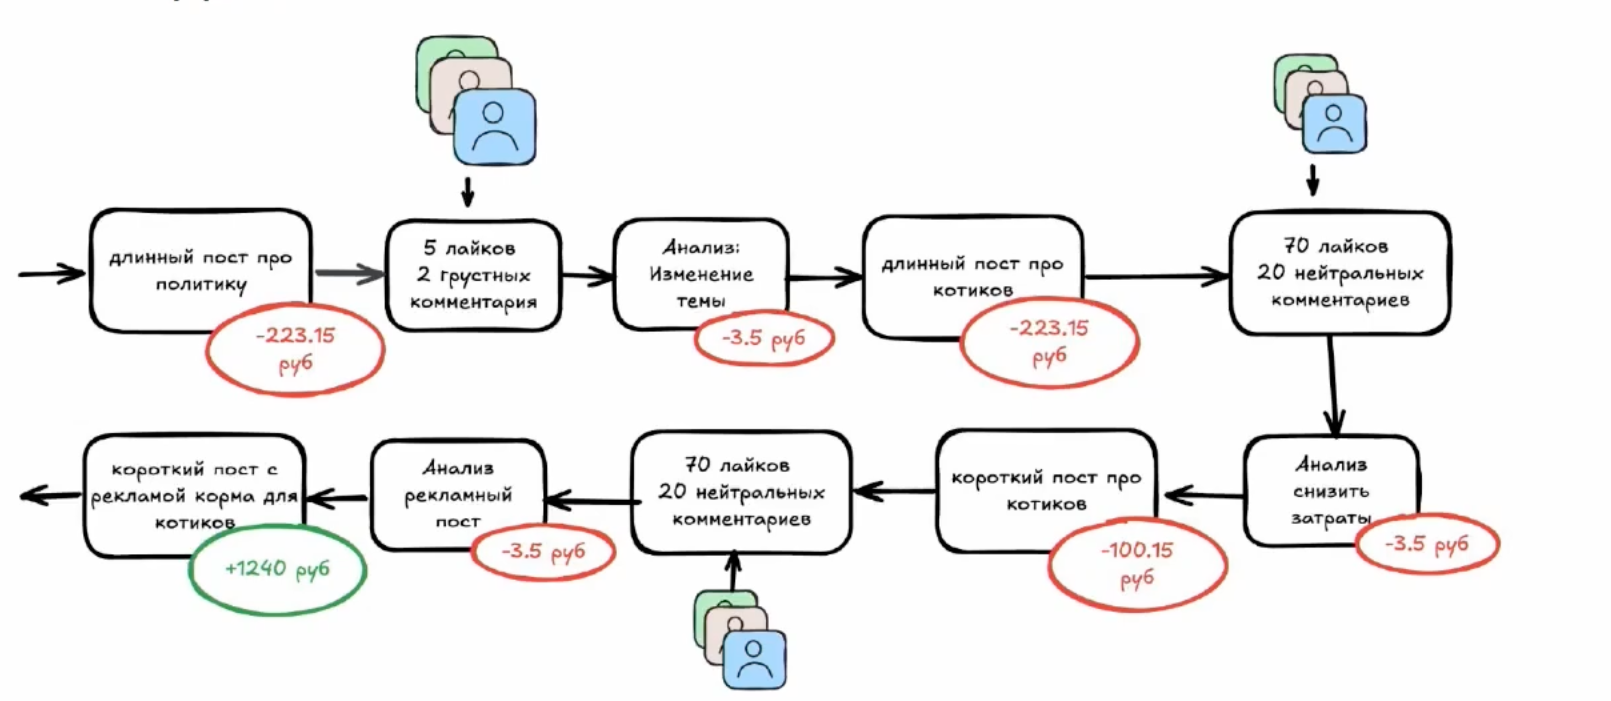
\includegraphics[width=0.95\textwidth]{./assets/llm-social-agent.png}
  \caption{Фрагмент контурной стратегии принятия решений ИИ-блогером: реакция среды влияет на выбор темы, длины и типа постов, что в свою очередь определяет финансовый результат}
  \label{fig:ai-blogger-flow}
\end{figure}

Среда в данной системе включает в себя набор наблюдаемых параметров: поведенческие реакции пользователей (вовлечённость, время взаимодействия, отписки), алгоритмические отклики платформы (доставляемость, продвижение, ранжирование), а также метаинформацию о конкурентном фоне. Эти параметры формируют изменяющееся, частично стохастическое пространство, в рамках которого агент должен принимать решения. Среда не предоставляет чётких инструкций или прямой функции вознаграждения, а лишь генерирует сигналы обратной связи, через которые агент может судить о корректности своих действий.

Агент принимает решения в дискретном времени, публикуя сообщения, каждое из которых имеет структурированные признаки: тематику, формат, длину, эмоциональную окраску, наличие рекламных вставок и визуальные элементы. Особый интерес представляет параметр рекламной насыщенности — отношение прямой или нативной рекламы к общей плотности контента. Это значение влияет на немедленный доход агента, так как рекламные публикации напрямую связаны с оплатой, но одновременно снижает долгосрочную метрику вовлечённости, поскольку пользователи склонны снижать интерес при росте коммерческого давления.

Регулирующий механизм в этом случае реализуется как адаптивная стратегия, оптимизирующая параметры публикации на основе наблюдаемой реакции. Такой механизм может быть реализован как табличная политика, как динамическое обновление эмпирических вероятностей, или через функцию полезности, вычисляемую из данных. Например, агент может формировать распределение предпочтений аудитории относительно интервалов между рекламными вставками, соотношения развлекательного и образовательного контента, или длины публикаций. Это распределение используется для взвешенного выбора параметров следующего сообщения.

Важно, что оптимальность здесь носит не глобальный характер, а локальный и адаптивный: агент не стремится к максимизации единой функции, а к сохранению устойчивого равновесия, в котором уровень охвата остаётся стабильным, а доходность публикаций превышает заданный порог. Если рекламная активность слишком высока, и охват начинает падать, агент корректирует стратегию в сторону «очищения» потока от навязчивых элементов, и наоборот — при длительном отсутствии дохода с рекламы усиливает коммерческую нагрузку.

В долгосрочной перспективе агент может также адаптировать собственную «персону» — менять стилистику, сферу тем или целевую аудиторию, если текущая конфигурация перестаёт быть эффективной. Таким образом, модель позволяет реализовать устойчивый контентный процесс, в котором ИИ-блогер ведёт себя как активный участник цифровой среды, балансируя между краткосрочной выгодой и долгосрочным доверием, без необходимости ручного управления или внешнего контроля.

% ## 5.3.2
\mysubsection{Найм сотрудников}

Процесс найма в современной цифровой среде можно представить как систему, функционирующую на основе взаимодействия множества агентов в условиях информационной асимметрии. В этом контексте каждый кандидат, подающий резюме, представляет собой агента, предлагающего определённый набор характеристик и сигналов. Работодатель, действующий как агрегирующий агент или модератор, формирует спрос, специфицируя набор желаемых свойств, зачастую неполно или неявно.

Средой выступает рынок труда как информационно-насыщенное, но шумное пространство, в которое непрерывно поступают новые данные в виде резюме, сопроводительных писем, тестовых заданий и поведенческих сигналов (например, частота смены мест работы, уровень соответствия требованиям, структура достижений). При этом объём входного потока велик: в случае публичной вакансии даже среднего уровня можно получить от нескольких сотен до десятков тысяч откликов, что делает ручную обработку экономически и организационно неэффективной.

Ключевая задача — выделить из потока релевантную подвыборку для дальнейшей более глубокой оценки. Это позволяет ввести механизм, основанный на предварительной фильтрации с применением языковой модели (LLM), обученной на примерах успешных и неуспешных кандидатов, и обладающей способностью извлекать латентные признаки из неструктурированных данных.

Агентом в этом случае становится LLM, действующая как автоматизированный предварительный оценщик. Она получает на вход резюме и сопутствующую информацию, а на выходе формирует вероятностную оценку пригодности (или относительный ранг) по заданной позиции. Модель может использовать доступные мета-данные работодателя (исторические успехи предыдущих сотрудников, специфика команды, задачи) в качестве контекста. Такая модель обучается не на универсальной задаче соответствия, а на конкретном распределении оценок в данной среде: то есть "учится у самого работодателя", подстраиваясь под его латентные предпочтения.

Механизмом выступает процедура агрегации и пороговой фильтрации. Например, все входящие резюме ранжируются по выходному сигналу модели, после чего отбираются верхние $k$\% для передачи в отдел подбора персонала. При этом граница отбора может адаптироваться в зависимости от динамики заявок, текущей загрузки рекрутеров, или доступного бюджета на найм. Если LLM предоставляет интерпретируемые признаки (например, «высокая релевантность ключевых навыков», «нестабильный карьерный путь», «редкие компетенции»), они могут быть использованы для объяснимости решений и формирования обратной связи.

Среда, как информационно-динамическая система, в данном случае не пассивна: поведение работодателей (например, отклики на кандидатов, реальные наймы) возвращается в систему в качестве сигнала корректности. Это позволяет встроить в цикл обучения модель с обратной связью — когда поведение агента постепенно адаптируется к новому распределению данных. Например, если обнаруживается, что модель недооценивает кандидатов с нетипичным бэкграундом, но они успешно проходят собеседования, веса признаков модели автоматически корректируются.

Таким образом, система переходит от однократного использования модели к непрерывному контекстуальному обучению: агент становится не просто фильтром, а активным участником процесса согласования интересов работодателя и кандидатов, формируя динамическую модель предпочтений.

Такой подход позволяет не только автоматизировать первичную фильтрацию, но и повысить прозрачность найма, уменьшить риск субъективных искажений и построить систему, в которой доверие к решению машины основывается на воспроизводимости и объяснимости. Модель «агент – среда – механизм» здесь раскрывает себя как формальная основа построения устойчивой, масштабируемой и обучаемой архитектуры цифрового рекрутинга.

% ## 5.3.3
\mysubsection{Вендинговый апарат}

Вендинговый аппарат, наделённый возможностью самостоятельно определять цены и адаптироваться к изменяющемуся спросу, представляет собой автономного агента, взаимодействующего с физической и поведенческой средой. Он не просто исполняет заранее заданные инструкции, но и реагирует на сигналы от потребителей, адаптирует стратегию ценообразования, регулирует ассортимент и вырабатывает эмпирические правила поведения на основе накопленных данных. Такой агент может функционировать как элемент децентрализованной торговли, принимающий решения в условиях неопределённости и ограниченной обратной связи.

Среда в данном случае состоит из потока потребительских взаимодействий, а также внешних переменных — времени суток, сезонных колебаний, характеристик местоположения и конкуренции. Данные параметры влияют на вероятность покупки и отклик на изменение цен, но они не всегда доступны напрямую. Поэтому среда воспринимается аппаратом опосредованно, через изменения показателей спроса и выручки.

На первый взгляд может показаться, что использование крупной языковой модели (LLM), интегрированной в логику управления аппаратом, способно обеспечить необходимую адаптивность и гибкость. Действительно, LLM может извлекать сигналы из неструктурированных данных (например, жалоб, запросов на товары), интерпретировать тенденции и генерировать предложения по корректировке цен. Однако одного лишь применения LLM-агента недостаточно для устойчивого поведения.

Это продемонстрировано в исследовании Market Simulation for LLM Agents (Chen et al., 2024), в котором LLM используются в роли экономических агентов — потребителей, поставщиков и инвесторов — в симулированной рыночной среде. В результате наблюдается интересное поведение: модели демонстрируют склонность к стратегическому ценообразованию, реагируют на дефицит и даже участвуют в зачаточной форме спекуляции. Тем не менее, авторы приходят к выводу, что без внешнего управляющего компонента поведение LLM-агентов быстро становится нестабильным.

Среди выявленных ограничений особенно значимы три. Во-первых, LLM не обладают устойчивой памятью о собственных действиях или о состоянии среды, так как работают в stateless-режиме — каждый запрос обрабатывается изолированно от предыдущих, что исключает формирование долгосрочной стратегии. Во-вторых, LLM не обеспечивают глобальной оптимальности: даже если каждая реакция локально разумна, их совокупность может не приводить к устойчивому равновесию, особенно если и другие агенты обучаются параллельно. И наконец, в условиях рыночной турбулентности модели демонстрируют поведение, подверженное стахастическим флуктуациям, переобучению на шум и искажению при краткосрочном усилении сигналов.


Таким образом, необходимо ввести механизм управления, выполняющий три критически важных функции:

\begin{itemize}
  \item Поддержка целостной среды — моделирование ресурсов, ограничений, последствий действий, чтобы обеспечить устойчивость экономики.
  \item Агрегация и фильтрация сигналов — отслеживание мета-показателей (снижение спроса, перегрев рынка, рост дефицита), недоступных отдельным агентам.
  \item Изменение правил взаимодействия — введение локинга, корректировка штрафов, ограничение действий или адаптация стратегий для стабилизации поведения агентов.
\end{itemize}

В контексте вендингового аппарата это означает, что поверх LLM-агента необходимо задать механизм регулирования — систему метаправил, регулирующих интервал смены цен, ограничение частоты корректировок, допустимые диапазоны цен и пороги срабатывания адаптации. Такой механизм позволяет избежать сценариев, при которых автомат начинает чрезмерно часто менять цену, реагируя на шум, либо не способен отреагировать на структурные изменения, например, появление конкурента или смену потребительского паттерна.

Интеграция управляющего компонента в архитектуру «агент – среда – механизм» позволяет вендинговому аппарату не просто адаптироваться к текущей среде, но и участвовать в устойчивом и предсказуемом рыночном взаимодействии. LLM в этом случае выступает как вычислительный агент с обобщёнными знаниями, а механизм управления задаёт долгосрочную рамку и удерживает поведение в границах рациональности, необходимой для устойчивой микроэкономики.


% ## 5.3.4
\mysubsection{Оценка проектов}

Контесты по интеллектуальной оценке представляют собой особый тип среды, в которой агенты (в том числе основанные на языковых моделях) соревнуются не за ресурсы в прямом смысле, а за точность приближения к скрытой цели — эталонной оценке. Это принципиально иной формат взаимодействия: в отличие от рынка, где поведение агента влияет на траекторию будущих состояний среды, здесь среда на время фиксирована, а взаимодействие между агентами реализуется через косвенное сравнение их стратегий.

В качестве примера можно рассмотреть контест на платформе Pond, где задачей является оценка релевантности объектов, вклада участников или качества предложений. Участникам предоставляется большое множество примеров без маркировки, и предлагается ранжировать их или присвоить численные оценки. После сбора всех предсказаний небольшая часть выборки сравнивается с эталоном, предоставленным экспертами или внешними источниками. Таким образом, агенты конкурируют за то, чтобы угадать скрытую функцию, минимизируя расхождение с ground truth на валидационном подмножестве.

Такая система естественным образом укладывается в архитектуру «агент – среда – механизм». Агентом здесь является LLM-модель или её конфигурация (с определённой температурой, шаблоном prompt'а, памятью, длиной контекста и т.д.), которая принимает решение о значении оценки для каждого объекта. Среда — это зафиксированное множество примеров, не поддающееся прямому воздействию со стороны агента. Важным отличием такой среды является её замороженность: действия агентов не изменяют её состояние, но изменяют распределение суждений о ней. В этом смысле контест можно интерпретировать как многослойную среду, в которой текущая среда вложена в более широкую — систему контеста, где поведение агентов агрегируется и анализируется.


Современные языковые модели (LLM) открывают новые возможности для оценки и фильтрации стартап-идей на ранних стадиях, особенно в условиях информационной асимметрии, когда полнота и точность данных ограничены. Аналогично роли бизнес-ангелов, описанной в работе \cite{lange2024angels}, LLM-системы могут выполнять функцию предварительной интеллектуальной фильтрации, позволяя автоматизировать процессы отбора, анализа и сопровождения инновационных проектов.

Контест на pond является подобной средой со скрытым механизмом оценки
Можем выбрать архитектуру или метрики для LLM модели

Примерами таких соревнований являются:

Экспериментальные соревнования, проведённые в рамках проектов \cite{cryptopond2025gg23} и \cite{cryptopond2025quantifying}, демонстрируют использование представленного метода, основанных на частично заданных эталонных ответах и агрегировании предсказаний участников. Центральной задачей этих контестов выступает распределение некоторой количественной величины (например, вклада участников в проект или релевантности объектов) по широкому множеству примеров, где прямое ручное аннотирование всего массива данных непрактично. Предлагаемый метод позволяет обойти это ограничение за счёт выборочного аннотирования небольшой подвыборки с последующим обучением на ней механизма агрегации.

На основе за \cite{lange2024angels}

\begin{figure}[H]
  \centering
  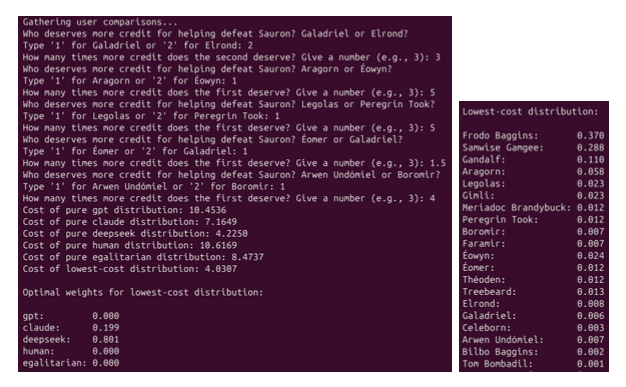
\includegraphics[width=0.5\textwidth]{./assets/llmcontest.png}
  \caption{Сравнение предел централизации и придела децентрализации}
  \label{fig:llmcontest}
\end{figure}

Первым этапом является генерация оценок полного множества. Участникам (в том числе LLM-моделям или их гибридным конфигурациям) предлагается самостоятельно сформировать полный список численных оценок по всем экземплярам заданного множества. Например, участник должен оценить степень вклада каждого из $n$ агентов в некоторый проект. Модели не ограничиваются по способу получения ответа: допустимы как прямые алгоритмические предсказания, так и использование внешних источников, цепочек рассуждений, или даже краудсорсинг третьих агентов.

Вторым этапом является создание эталона (ground truth subset). Независимая экспертная комиссия (жюри) предоставляет «эталон» --- небольшой поднабор ручных или полуавтоматических оценок, охватывающий малую часть исходного множества (например, 100 из 10 000 позиций). Эти оценки считаются высококачественными и выступают основой для проверки точности предсказаний. Независимая экспертная комиссия (жюри) предоставляет «эталон» --- небольшой поднабор ручных или полуавтоматических оценок, охватывающий малую часть исходного множества (например, 100 из 10 000 позиций). Эти оценки считаются высококачественными и выступают основой для проверки точности предсказаний.

После получения всех поданных списков проводится численная процедура сопоставления для определения наилучшего приближения: каждая предсказанная последовательность сравнивается с эталоном, и выбирается такая линейная комбинация предсказаний, которая минимизирует среднеквадратичную ошибку по выборке эталонных значений. Пусть $x_1, \dots, x_k$ --- это векторы оценок, поданные участниками, а $y_{\text{true}}$ --- эталонные оценки. Задача сводится к нахождению коэффициентов $\alpha_1, \dots, \alpha_k$, таких что:
\[
  \min_{\substack{\alpha_i \ge 0 \\ \sum_{i=1}^k \alpha_i = 1}}
  \Bigl\lVert \sum_{i=1}^k \alpha_i x_i - y_{\text{true}} \Bigr\rVert_2^2.
\]

Решение этой задачи определяет не только итоговую агрегацию, но и относительное вознаграждение (или доверие), которое получает каждый участник за своё предсказание.

Полученная комбинация $\hat{y} = \sum \alpha_i x_i$ принимается как финальный ответ системы --- агрегированная оценка по всему множеству объектов, максимально согласующаяся с мнением жюри на ограниченной выборке. При этом точечные ответы, которые наиболее точно отражают локальные закономерности в эталоне, получают больший вес в линейной смеси, независимо от их абсолютной производительности по всему корпусу.

\mysection{Вывод по пятой главе}

% Про вложенность
Соединение воедино рассмотренных вложенных друг в друга сред, где агенты соревнуются друг с другом открывает возможности для маштабирования.
Хотя формально консенсус невозможен, вложенность позволит находить локальные оптимумы. %% TODO: про вложенность
Разработка такой системы для блокчейн принесет приемущества и вероятно откроет не только экономические применения

% ###################################################
% ## Заключение
% ###################################################

\newpage
\begin{center}
  \textbf{ЗАКЛЮЧЕНИЕ}
\end{center}
\addcontentsline{toc}{chapter}{ЗАКЛЮЧЕНИЕ}

В рамках данной дипломной работы была разработана и исследована инвестирования в ранние стадии стартапов. Работа была направлена на решение структурных проблем существующих решений для превлечения ресуров, включая информационную асимметрию, субъективность оценок и риски для интеллектуальной собственности.

Практическая значимость разработанной платформы заключается в создании новой парадигмы инвестирования, которая имеет потенциал для преодоления структурных ограничений существующих механизмов и обеспечения более эффективного распределения ресурсов для инновационных проектов. Это может способствовать ускорению технологического развития, созданию новых рабочих мест и повышению глобальной конкурентоспособности экономики.

Проведенное исследование также выявило ряд направлений для дальнейшей работы, включая совершенствование криптоэкономических механизмов, развитие технологий защиты интеллектуальной собственности, улучшение методов оценки проектов, исследование социально-экономических эффектов и развитие регуляторных подходов.

В целом, результаты работы демонстрируют значительный потенциал интеграции блокчейн-технологий, искусственного интеллекта и инновационных экономических механизмов для трансформации системы венчурного инвестирования в направлении большей эффективности, справедливости и доступности. Разработанная платформа представляет собой не просто технологическое решение, но комплексный подход к переосмыслению процессов распределения ресурсов для инновационных проектов, что имеет стратегическое значение для развития экономики знаний и инноваций.

В итоге, все поставленные задачи были успешно решены.

\renewcommand{\bibname}{\fontsize{14pt}{21pt}\selectfont СПИСОК ИСПОЛЬЗОВАННЫХ ИСТОЧНИКОВ}
\bibliographystyle{bibformat}
\bibliography{bibliography}

\end{document}